% !TeX spellcheck = en_US
%\documentclass[11pt,a4paper]{article}
\documentclass[11pt
  , a4paper
  , article
  , oneside
%  , twoside
%  , draft
]{memoir}

\usepackage{control}
\usepackage[numbers]{natbib}


\begin{document}

\newcommand{\technumber}{
  RAON Control-Document Series\\
  Revision : v1.0,   Release : 2015-03-16 fixed date}
\title{\textbf{SRF Test Facility - Storage 시스템 구성}}

\author{이상일\thanks{silee7103@ibs.re.kr}, 이정한, 손창욱, 손형주, 박미정, 남승희 \\

  Rare Isotope Science Project\\
  Institute for Basic Science, Daejeon, South Korea
}
\date{\today}

\renewcommand{\maketitlehooka}{\begin{flushright}\textsf{\technumber}\end{flushright}}
%\renewcommand{\maketitlehookb}{\centering\textsf{\subtitle}}
%\renewcommand{\maketitlehookc}{C}
%\renewcommand{\maketitlehookd}{D}

\maketitle

\begin{abstract}
RAON is a particle accelerator to research the interaction between the nucleus forming a rare isotope as Korean heavy-ion accelerator. RAON accelerator consists of a number of facilities and equipments as a large-scaled experimental device operating under the distributed environment. 

ECR Ion source 및 RFQ Test를 위하여 문지동 카이스트 캠퍼스에 마련되 SRF Test Facility 건물에는 해당 장치의 Test시 발생하는 EPICS IOC 데이터를 저장하기 위한 목적으로 Storage 시스템이 구축되었다. 본 스토리지 시스템은 본 사이트에서 운영될 스토리지 시스템과 유사한 목적으로 가속기 실운영 환경하에서 스토리지 시스템은 운영 및 데이터 저장 성능에 대한 검증을 목적으로 한다. 본 문서에서는 SRF Test Facility 에서 운영될 스토리지 시스템의 구성에 대하여 상세 기술한다.

\end{abstract}

본 스토리지 시스템의 모델 및 사양은 아래와 같다.

\begin{lstlisting}[style=termstyle]
Dell Compellent SC4020 (Main Stroage System)
- SC4020, 32GB Memory
- Compellent SC4020 Controller x 2ea
- Dell 1TB, SAS, 6Gb, 2.5", 7.2K, HDD x 12ea
- SW, Storage Center OS Core Base License
- 3 year Warranty

PowerEdge R720 (Data Archiving Server)
- Intel Xeon Processor E5 - 2650 v2 2.6GHz, 20MCache, 8.0GTs QPI, 8C x 1ea
- 32GB (8GB RDIMM, 1600MT/s x 4ea)- 2TB 7.2K Near Line SAS x 2ea
- 300GB 10K RPM SAS 6Gbps x 2ea
- H710p Raid Controller, 1GB Cache
- 1GbE NIC x 4ea- Dual, Hot-plug, Redundant Power Supply (1+1), 750W- 3 year Warranty

Dell Brocade 300 8Gb FC Switch (SAN Switch)
- 16 Port with SFP+ GBIC
- 3 year Warranty

\end{lstlisting}

스토리지 시스템 구성에서 가장 중요한 구성 요소는 SAN Switch와의 연결 구성이며, 아래와 같이 구성 되었다.

\begin{lstlisting}[style=termstyle]
Switch Information Report for SW300

List of Switches

Switch ID   Worldwide Name           Enet IP Addr    FC IP Addr      Name
-------------------------------------------------------------------------
1: fffc01 10:00:00:27:f8:df:f3:c8 192.168.1.53    0.0.0.0        >"SW300"


Current Switch Information

Ethernet IP Address: 192.168.1.53
Ethernet Subnetmask: 255.255.255.0
Fibre Channel IP Address: 0.0.0.0
Fibre Channel Subnetmask: 0.0.0.0
Gateway Address: 192.168.1.1
Ethernet IPv6 Addresses: 

Kernel:     2.6.14.2   
Fabric OS:  v7.1.0a
Made on:    Tue Jan 22 19:37:11 2013
Flash:	    Thu Jan 30 19:54:48 2014
BootProm:   1.0.10
List of Inter-Switch Links

Local Domain ID: 1

Local Port     Domain     Remote Port     State
-------------------------------------------------------
List of Ports

switchName:	SW300
switchType:	71.2
switchState:	Online   
switchMode:	Native
switchRole:	Principal
switchDomain:	1
switchId:	fffc01
switchWwn:	10:00:00:27:f8:df:f3:c8
zoning:		ON (sw300)
switchBeacon:	OFF

Index Port Address Media Speed       State   Proto
==================================================
0   0   010000   id    N8	   Online      FC  F-Port  1 N Port + 1 NPIV public 
1   1   010100   id    N8	   Online      FC  F-Port  1 N Port + 1 NPIV public 
2   2   010200   id    N8	   Online      FC  F-Port  21:00:00:24:ff:4a:b8:b8 
3   3   010300   id    N8	   No_Light    FC  
4   4   010400   id    N8	   No_Light    FC  
5   5   010500   id    N8	   No_Light    FC  
6   6   010600   id    N8	   No_Light    FC  
7   7   010700   id    N8	   No_Light    FC  
8   8   010800   id    N8	   Online      FC  F-Port  1 N Port + 1 NPIV public 
9   9   010900   id    N8	   Online      FC  F-Port  1 N Port + 1 NPIV public 
10  10   010a00   id    N8	   Online      FC  F-Port  21:00:00:24:ff:4a:b8:b9 
11  11   010b00   id    N8	   No_Light    FC  
12  12   010c00   id    N8	   No_Light    FC  
13  13   010d00   id    N8	   No_Light    FC  
14  14   010e00   id    N8	   No_Light    FC  
15  15   010f00   id    N8	   No_Light    FC  
16  16   011000   --    N8	   No_Module   FC  (No POD License) Disabled
17  17   011100   --    N8	   No_Module   FC  (No POD License) Disabled
18  18   011200   --    N8	   No_Module   FC  (No POD License) Disabled
19  19   011300   --    N8	   No_Module   FC  (No POD License) Disabled
20  20   011400   --    N8	   No_Module   FC  (No POD License) Disabled
21  21   011500   --    N8	   No_Module   FC  (No POD License) Disabled
22  22   011600   --    N8	   No_Module   FC  (No POD License) Disabled
23  23   011700   --    N8	   No_Module   FC  (No POD License) Disabled
Name Server

{
010000 010001 010100 010101 010200 010800 010801 010900 
010901 010a00 
10 Nx_Ports in the Fabric } 

{
Type Pid    COS     PortName                NodeName                 TTL(sec)
N    010000;      3;50:00:d3:10:00:86:d6:05;50:00:d3:10:00:86:d6:00; na
FC4s: FCP 
PortSymb: [90] "Compellent Port QLGC FC 8Gbps; Slot=01 Port=01 in Controller: SN 34518 of Storage Center: "
NodeSymb: [47] "Compellent Storage Center: Storage Center 34518"
Fabric Port Name: 20:00:00:27:f8:df:f3:c8 
Permanent Port Name: 50:00:d3:10:00:86:d6:05
Port Index: 0
Share Area: No
Device Shared in Other AD: No
Redirect: No 
Partial: No
LSAN: No
N    010001;      3;50:00:d3:10:00:86:d6:1f;50:00:d3:10:00:86:d6:01; na
FC4s: FCP 
PortSymb: [110] "Compellent Port QLGC FC 8Gbps; Slot=01 Port=01 in Controller: SN 34518 of Storage Center: Storage Center 34518"
NodeSymb: [47] "Compellent Storage Center: Storage Center 34518"
Fabric Port Name: 20:00:00:27:f8:df:f3:c8 
Permanent Port Name: 50:00:d3:10:00:86:d6:05
Port Index: 0
Share Area: No
Device Shared in Other AD: No
Redirect: No 
Partial: No
LSAN: No
N    010100;      3;50:00:d3:10:00:86:d6:12;50:00:d3:10:00:86:d6:00; na
FC4s: FCP 
PortSymb: [110] "Compellent Port QLGC FC 8Gbps; Slot=01 Port=01 in Controller: SN 34519 of Storage Center: Storage Center 34518"
NodeSymb: [47] "Compellent Storage Center: Storage Center 34518"
Fabric Port Name: 20:01:00:27:f8:df:f3:c8 
Permanent Port Name: 50:00:d3:10:00:86:d6:12
Port Index: 1
Share Area: No
Device Shared in Other AD: No
Redirect: No 
Partial: No
LSAN: No
N    010101;      3;50:00:d3:10:00:86:d6:21;50:00:d3:10:00:86:d6:02; na
FC4s: FCP 
PortSymb: [110] "Compellent Port QLGC FC 8Gbps; Slot=01 Port=01 in Controller: SN 34519 of Storage Center: Storage Center 34518"
NodeSymb: [47] "Compellent Storage Center: Storage Center 34518"
Fabric Port Name: 20:01:00:27:f8:df:f3:c8 
Permanent Port Name: 50:00:d3:10:00:86:d6:12
Port Index: 1
Share Area: No
Device Shared in Other AD: No
Redirect: No 
Partial: No
LSAN: No
N    010200;      3;21:00:00:24:ff:4a:b8:b8;20:00:00:24:ff:4a:b8:b8; na
FC4s: FCP 
NodeSymb: [37] "QLE2562 FW:v5.04.01 DVR:v8.03.07.12-k"
Fabric Port Name: 20:02:00:27:f8:df:f3:c8 
Permanent Port Name: 21:00:00:24:ff:4a:b8:b8
Port Index: 2
Share Area: No
Device Shared in Other AD: No
Redirect: No 
Partial: No
LSAN: No
N    010800;      3;50:00:d3:10:00:86:d6:06;50:00:d3:10:00:86:d6:00; na
FC4s: FCP 
PortSymb: [90] "Compellent Port QLGC FC 8Gbps; Slot=01 Port=02 in Controller: SN 34518 of Storage Center: "
NodeSymb: [47] "Compellent Storage Center: Storage Center 34518"
Fabric Port Name: 20:08:00:27:f8:df:f3:c8 
Permanent Port Name: 50:00:d3:10:00:86:d6:06
Port Index: 8
Share Area: No
Device Shared in Other AD: No
Redirect: No 
Partial: No
LSAN: No
N    010801;      3;50:00:d3:10:00:86:d6:20;50:00:d3:10:00:86:d6:01; na
FC4s: FCP 
PortSymb: [110] "Compellent Port QLGC FC 8Gbps; Slot=01 Port=02 in Controller: SN 34518 of Storage Center: Storage Center 34518"
NodeSymb: [47] "Compellent Storage Center: Storage Center 34518"
Fabric Port Name: 20:08:00:27:f8:df:f3:c8 
Permanent Port Name: 50:00:d3:10:00:86:d6:06
Port Index: 8
Share Area: No
Device Shared in Other AD: No
Redirect: No 
Partial: No
LSAN: No
N    010900;      3;50:00:d3:10:00:86:d6:13;50:00:d3:10:00:86:d6:00; na
FC4s: FCP 
PortSymb: [110] "Compellent Port QLGC FC 8Gbps; Slot=01 Port=02 in Controller: SN 34519 of Storage Center: Storage Center 34518"
NodeSymb: [47] "Compellent Storage Center: Storage Center 34518"
Fabric Port Name: 20:09:00:27:f8:df:f3:c8 
Permanent Port Name: 50:00:d3:10:00:86:d6:13
Port Index: 9
Share Area: No
Device Shared in Other AD: No
Redirect: No 
Partial: No
LSAN: No
N    010901;      3;50:00:d3:10:00:86:d6:22;50:00:d3:10:00:86:d6:02; na
FC4s: FCP 
PortSymb: [110] "Compellent Port QLGC FC 8Gbps; Slot=01 Port=02 in Controller: SN 34519 of Storage Center: Storage Center 34518"
NodeSymb: [47] "Compellent Storage Center: Storage Center 34518"
Fabric Port Name: 20:09:00:27:f8:df:f3:c8 
Permanent Port Name: 50:00:d3:10:00:86:d6:13
Port Index: 9
Share Area: No
Device Shared in Other AD: No
Redirect: No 
Partial: No
LSAN: No
N    010a00;      3;21:00:00:24:ff:4a:b8:b9;20:00:00:24:ff:4a:b8:b9; na
FC4s: FCP 
NodeSymb: [37] "QLE2562 FW:v5.04.01 DVR:v8.03.07.12-k"
Fabric Port Name: 20:0a:00:27:f8:df:f3:c8 
Permanent Port Name: 21:00:00:24:ff:4a:b8:b9
Port Index: 10
Share Area: No
Device Shared in Other AD: No
Redirect: No 
Partial: No
LSAN: No
The Local Name Server has 10 entries }
Zoning Information

Defined configuration:
cfg:	sw300	SC4020_FD01_P_ALL; SC4020_FD01_V_ALL; 
SC4020_FD01_V_ALL_srfdb_S6_P1; SC4020_FD02_P_ALL; 
SC4020_FD02_V_ALL; SC4020_FD02_V_ALL_srfdb_S6_P2
zone:	SC4020_FD01_P_ALL	
SC4020_C0_P1; SC4020_C1_P1
zone:	SC4020_FD01_V_ALL	
SC4020_C0_V1; SC4020_C1_V1
zone:	SC4020_FD01_V_ALL_srfdb_S6_P1	
SC4020_C0_V1; SC4020_C1_V1; srfdb_S6_P1
zone:	SC4020_FD02_P_ALL	
SC4020_C0_P2; SC4020_C1_P2
zone:	SC4020_FD02_V_ALL	
SC4020_C0_V2; SC4020_C1_V2
zone:	SC4020_FD02_V_ALL_srfdb_S6_P2	
SC4020_C0_V2; SC4020_C1_V2; srfdb_S6_P2
alias:	SC4020_C0_P1	
50:00:d3:10:00:86:d6:05
alias:	SC4020_C0_P2	
50:00:d3:10:00:86:d6:06
alias:	SC4020_C0_V1	
50:00:d3:10:00:86:d6:1f
alias:	SC4020_C0_V2	
50:00:d3:10:00:86:d6:20
alias:	SC4020_C1_P1	
50:00:d3:10:00:86:d6:12
alias:	SC4020_C1_P2	
50:00:d3:10:00:86:d6:13
alias:	SC4020_C1_V1	
50:00:d3:10:00:86:d6:21
alias:	SC4020_C1_V2	
50:00:d3:10:00:86:d6:22
alias:	srfdb_S6_P1	
21:00:00:24:ff:4a:b8:b8
alias:	srfdb_S6_P2	
21:00:00:24:ff:4a:b8:b9

Effective configuration:
cfg:	sw300	
zone:	SC4020_FD01_P_ALL	
50:00:d3:10:00:86:d6:05
50:00:d3:10:00:86:d6:12
zone:	SC4020_FD01_V_ALL	
50:00:d3:10:00:86:d6:1f
50:00:d3:10:00:86:d6:21
zone:	SC4020_FD01_V_ALL_srfdb_S6_P1	
50:00:d3:10:00:86:d6:1f
50:00:d3:10:00:86:d6:21
21:00:00:24:ff:4a:b8:b8
zone:	SC4020_FD02_P_ALL	
50:00:d3:10:00:86:d6:06
50:00:d3:10:00:86:d6:13
zone:	SC4020_FD02_V_ALL	
50:00:d3:10:00:86:d6:20
50:00:d3:10:00:86:d6:22
zone:	SC4020_FD02_V_ALL_srfdb_S6_P2	
50:00:d3:10:00:86:d6:20
50:00:d3:10:00:86:d6:22
21:00:00:24:ff:4a:b8:b9

SFP Serial ID Information

Port  0: id (sw) Vendor: BROCADE          Serial No: UAF414260001WGM  Speed: 2,4,8_Gbps 
Port  1: id (sw) Vendor: BROCADE          Serial No: UAF414260001WC5  Speed: 2,4,8_Gbps 
Port  2: id (sw) Vendor: BROCADE          Serial No: UAF414260001WFT  Speed: 2,4,8_Gbps 
Port  3: id (sw) Vendor: BROCADE          Serial No: UAF414260001WM4  Speed: 2,4,8_Gbps 
Port  4: id (sw) Vendor: BROCADE          Serial No: UAF414260001WGK  Speed: 2,4,8_Gbps 
Port  5: id (sw) Vendor: BROCADE          Serial No: UAF414260001WGU  Speed: 2,4,8_Gbps 
Port  6: id (sw) Vendor: BROCADE          Serial No: UAF414260001WEV  Speed: 2,4,8_Gbps 
Port  7: id (sw) Vendor: BROCADE          Serial No: UAF414260001WDD  Speed: 2,4,8_Gbps 
Port  8: id (sw) Vendor: BROCADE          Serial No: UAF41420000026E  Speed: 2,4,8_Gbps 
Port  9: id (sw) Vendor: BROCADE          Serial No: UAF41420000024A  Speed: 2,4,8_Gbps 
Port 10: id (sw) Vendor: BROCADE          Serial No: UAF41420000026W  Speed: 2,4,8_Gbps 
Port 11: id (sw) Vendor: BROCADE          Serial No: UAF414200000258  Speed: 2,4,8_Gbps 
Port 12: id (sw) Vendor: BROCADE          Serial No: UAF41420000024P  Speed: 2,4,8_Gbps 
Port 13: id (sw) Vendor: BROCADE          Serial No: UAF41420000024Z  Speed: 2,4,8_Gbps 
Port 14: id (sw) Vendor: BROCADE          Serial No: UAF41420000026B  Speed: 2,4,8_Gbps 
Port 15: id (sw) Vendor: BROCADE          Serial No: UAF41420000024V  Speed: 2,4,8_Gbps 
Port 16: -- 
Port 17: -- 
Port 18: -- 
Port 19: -- 
Port 20: -- 
Port 21: -- 
Port 22: -- 
Port 23: -- 
\end{lstlisting}

\clearpage

\chapter{Storage System}

\section{Architecture}
\begin{figure}[h!]
	\centering
	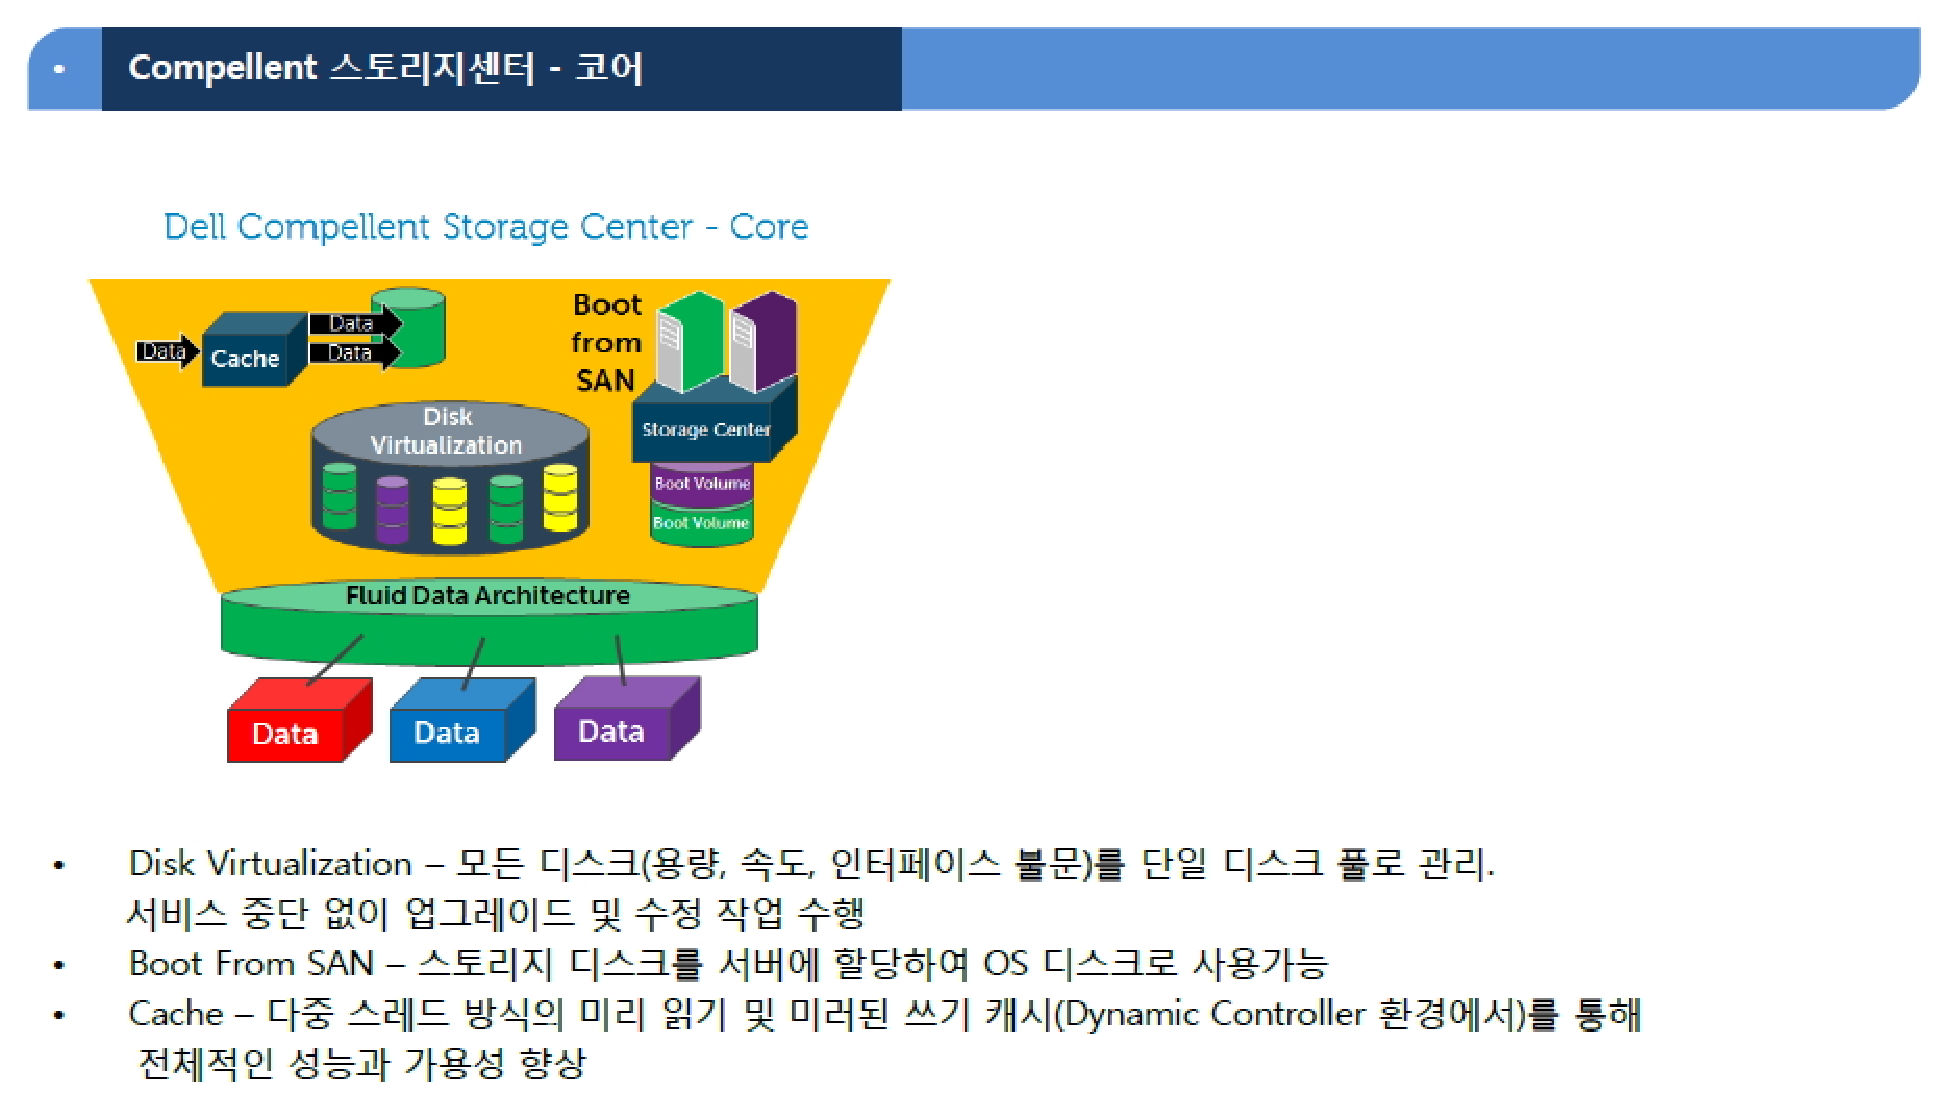
\includegraphics[width=0.85\textwidth]{./images/srfdb_storage_arch_1.eps}
	\caption{SRF Storage Architecture - 1}
	\label{fig:srfdb_arch_1} 
\end{figure}

\begin{figure}[h!]
	\centering
	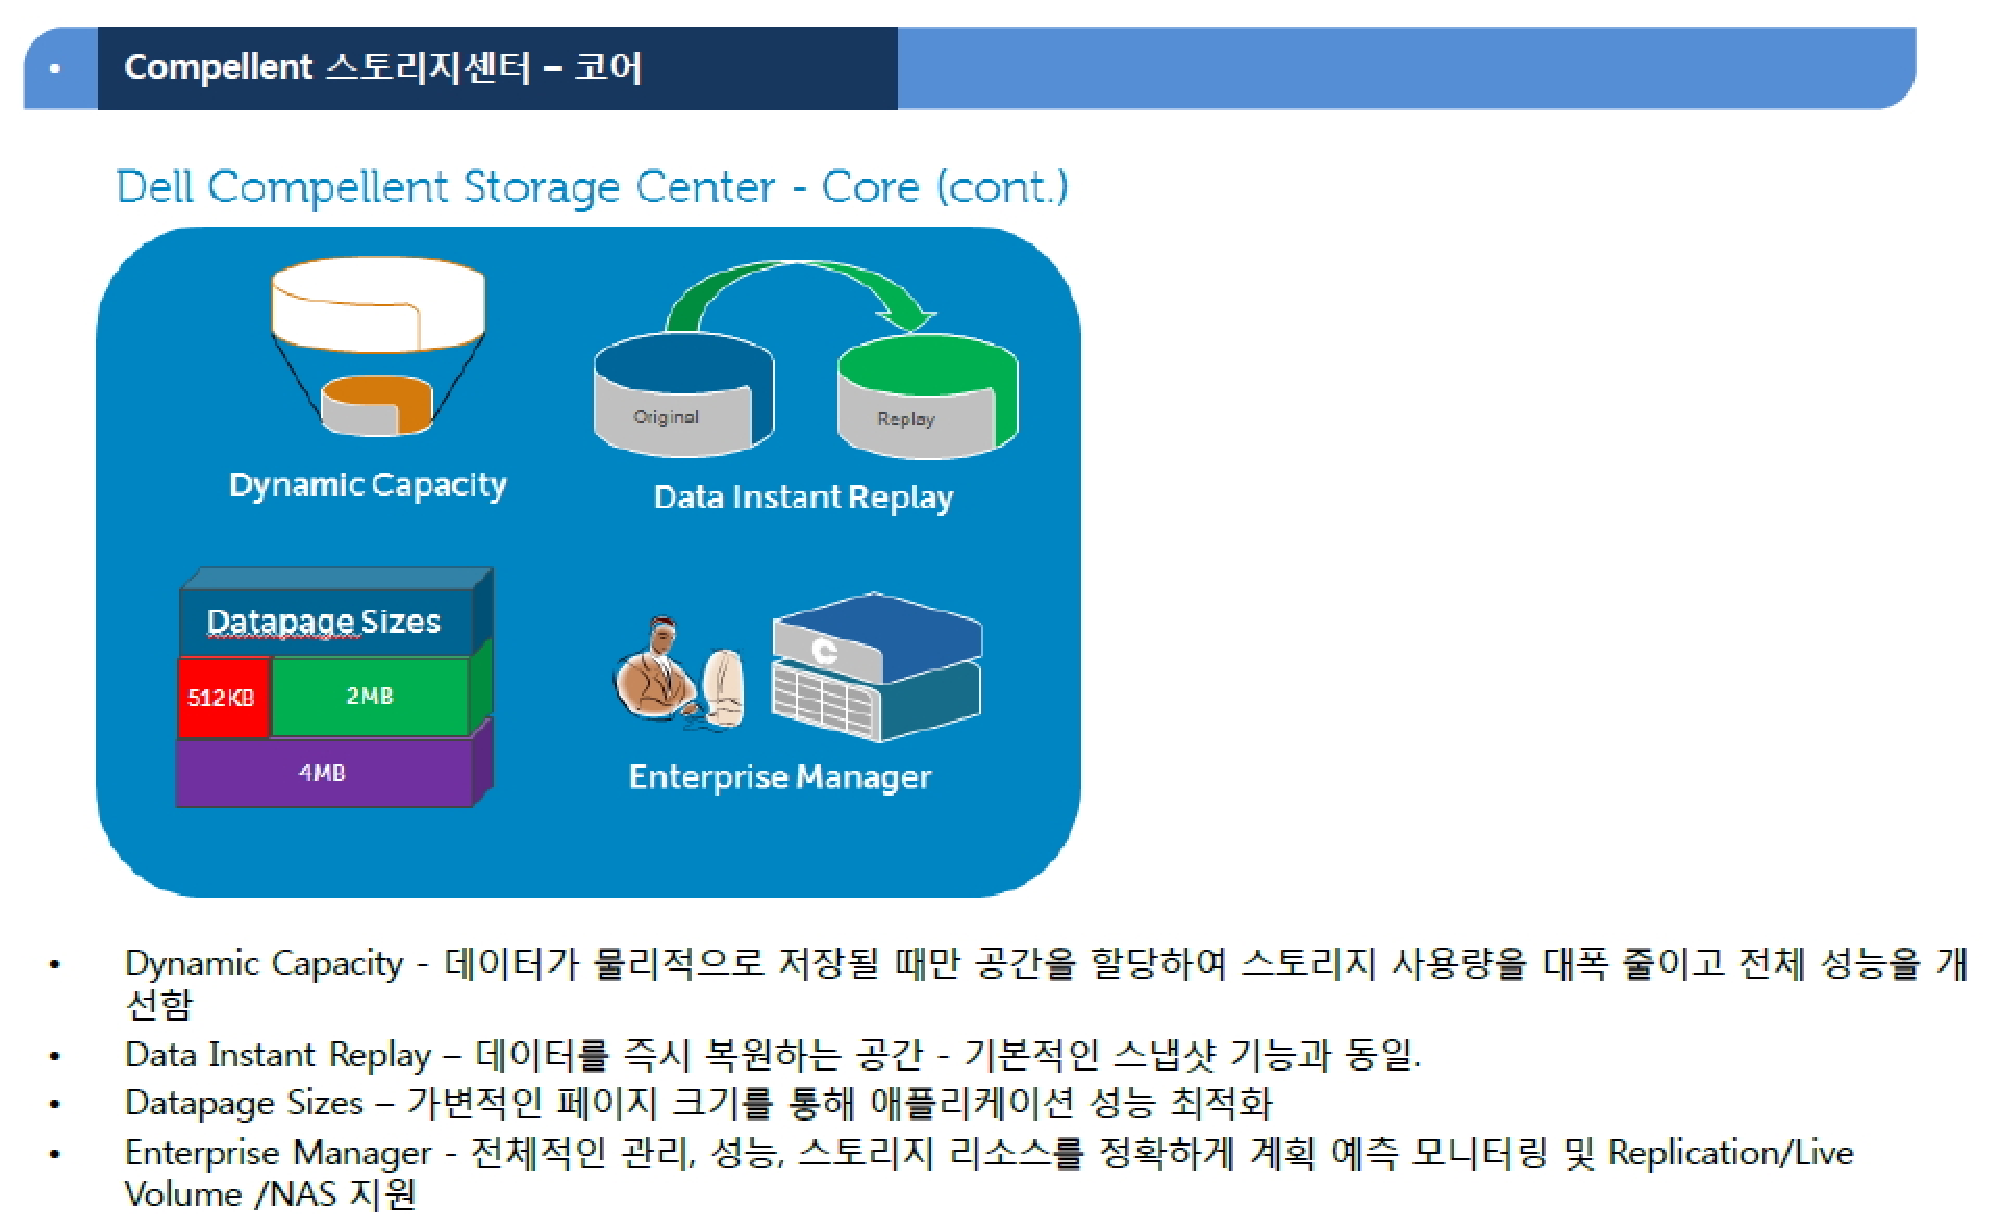
\includegraphics[width=0.85\textwidth]{./images/srfdb_storage_arch_2.eps}
	\caption{SRF Storage Architecture - 2}
	\label{fig:srfdb_arch_2} 
\end{figure}

\begin{figure}[h!]
	\centering
	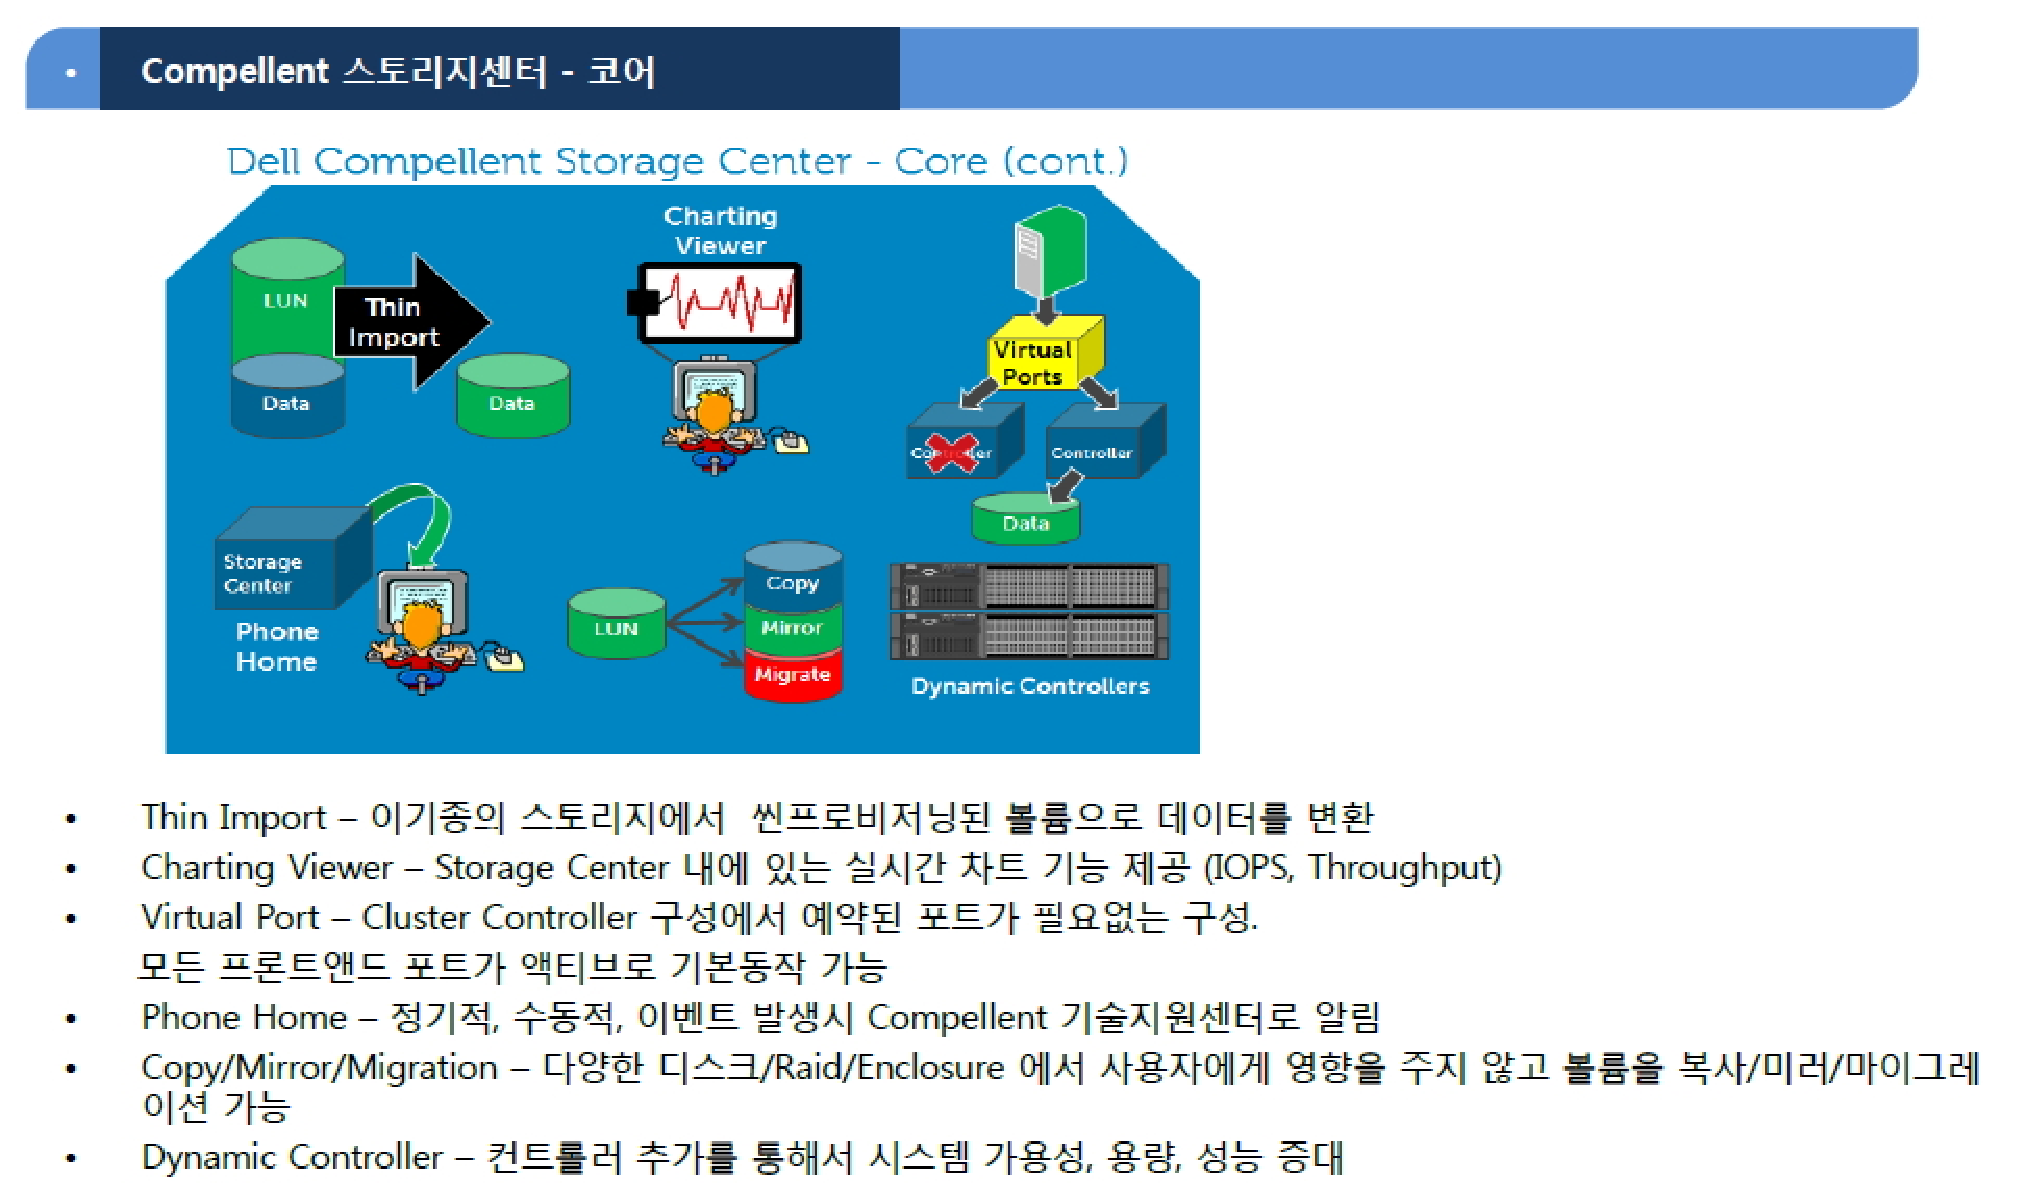
\includegraphics[width=0.85\textwidth]{./images/srfdb_storage_arch_3.eps}
	\caption{SRF Storage Architecture - 3}
	\label{fig:srfdb_arch_3} 
\end{figure}

\begin{figure}[h!]
	\centering
	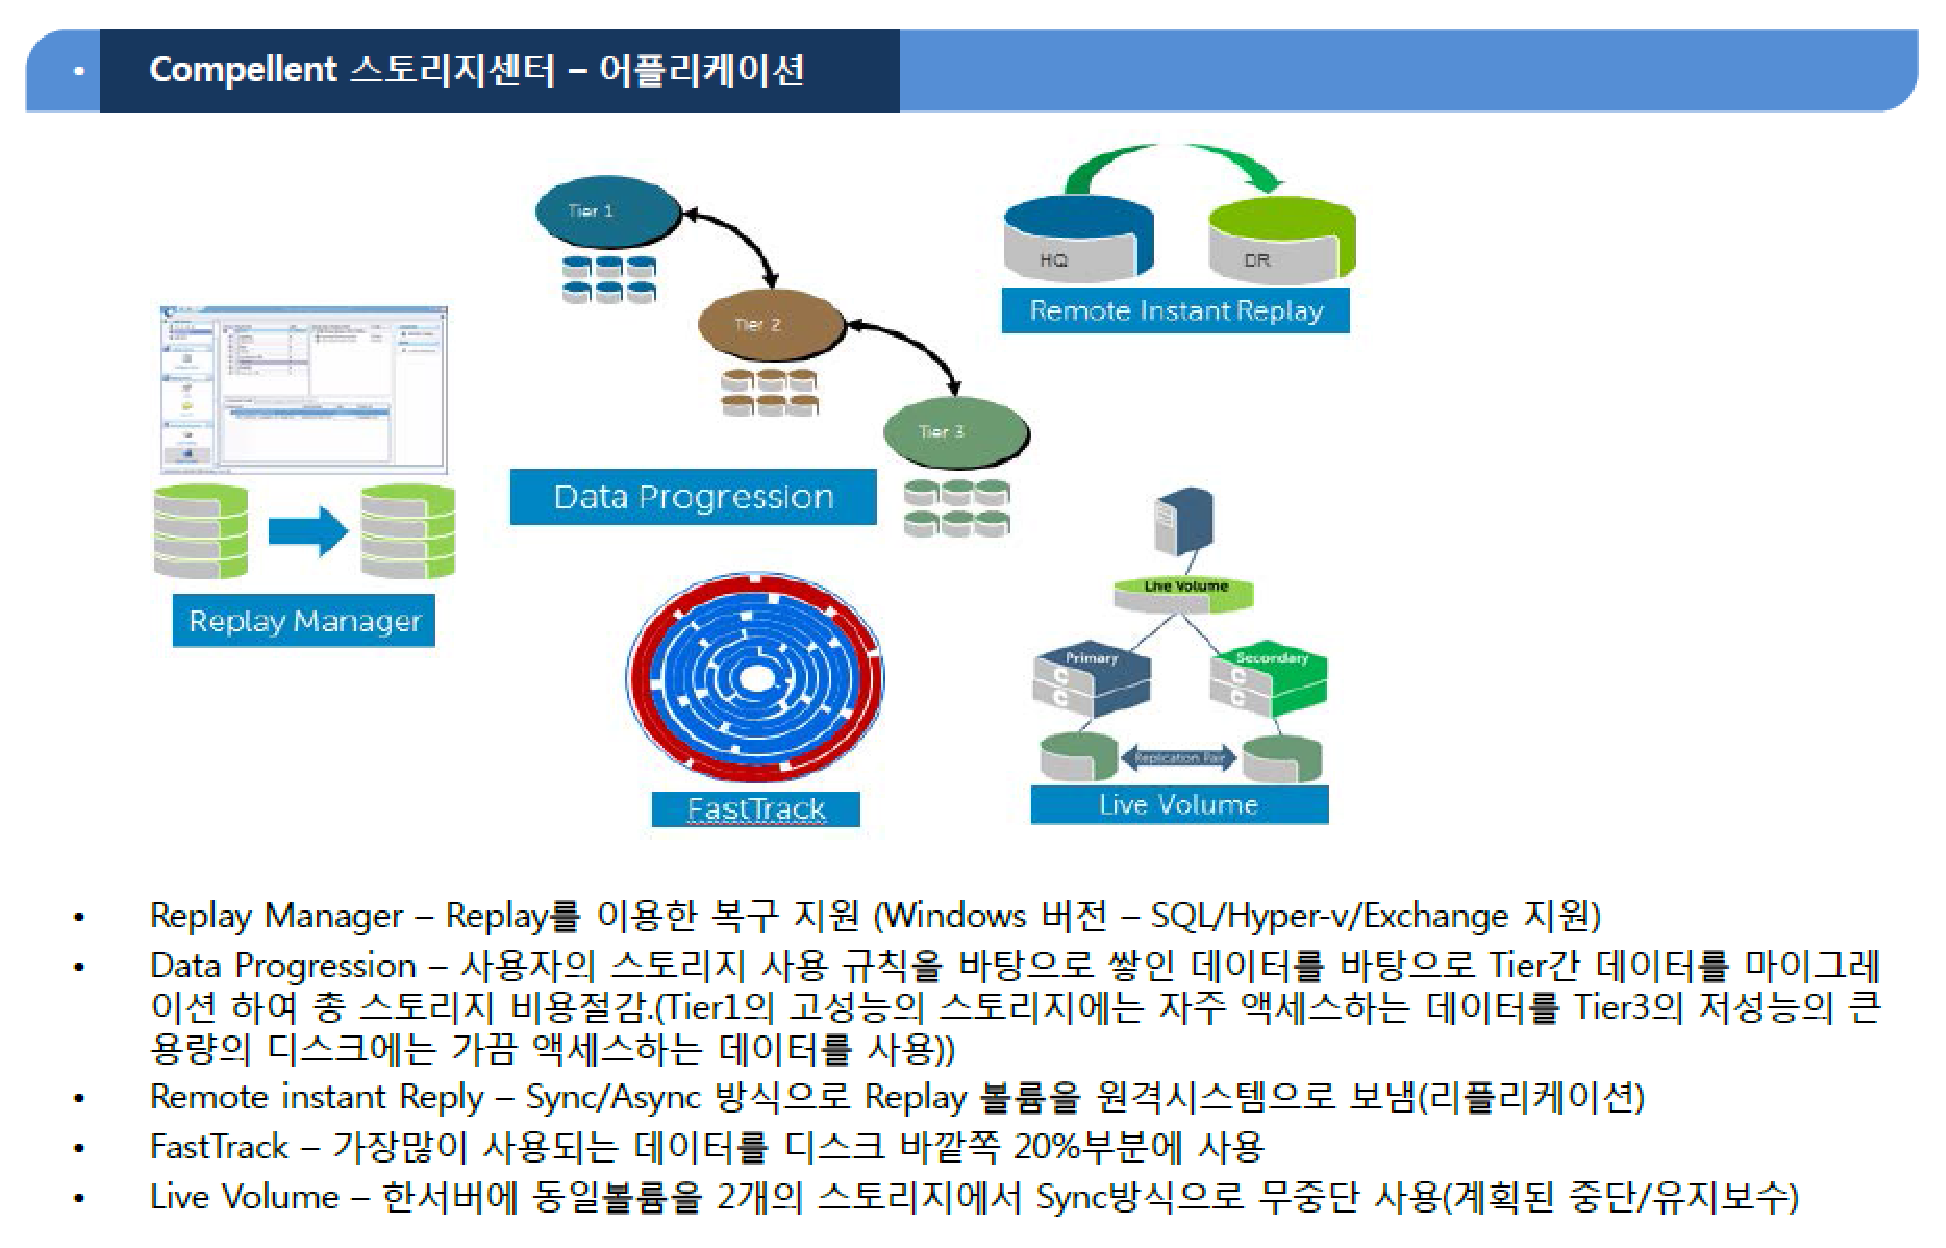
\includegraphics[width=0.85\textwidth]{./images/srfdb_storage_arch_4.eps}
	\caption{SRF Storage Architecture - 4}
	\label{fig:srfdb_arch_4} 
\end{figure}

\begin{figure}[h!]
	\centering
	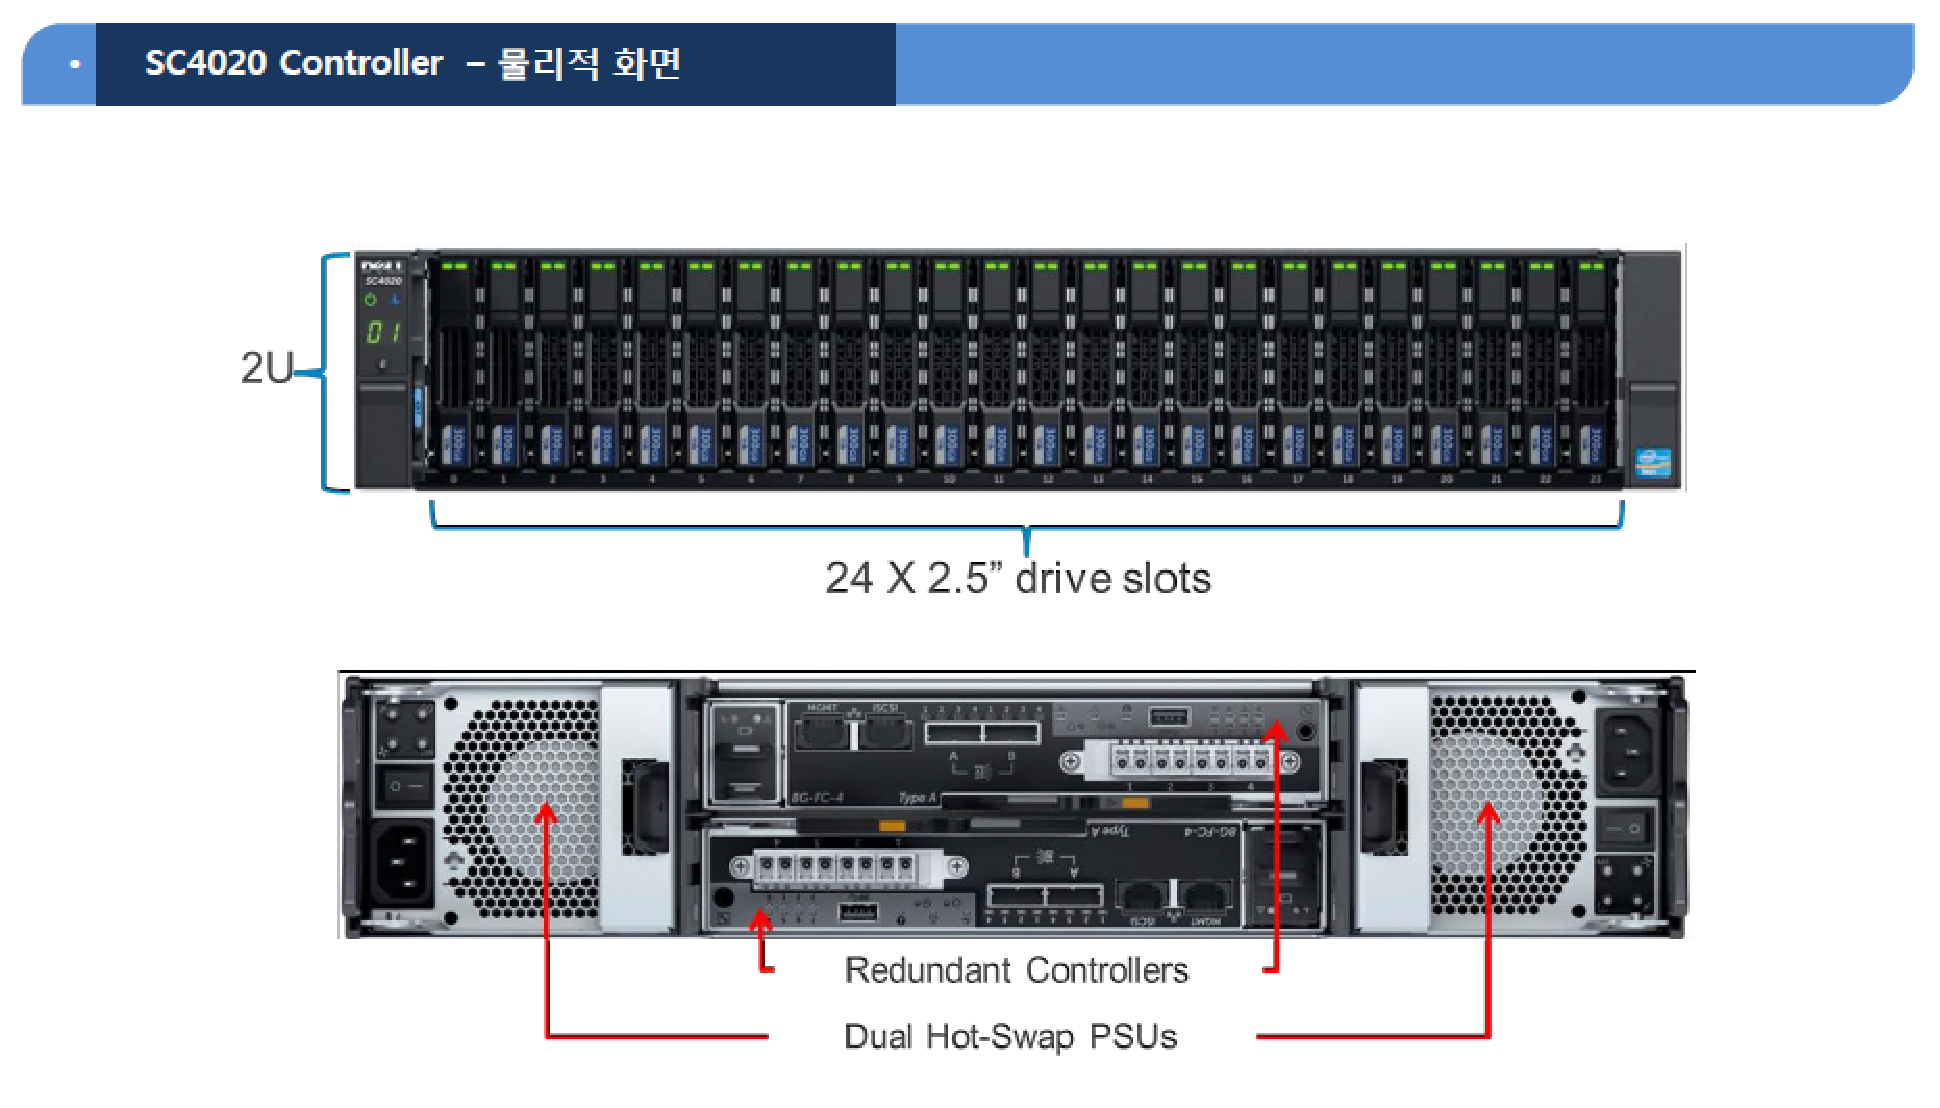
\includegraphics[width=0.85\textwidth]{./images/srfdb_storage_arch_5.eps}
	\caption{SRF Storage Architecture - 5}
	\label{fig:srfdb_arch_5} 
\end{figure}

\begin{figure}[h!]
	\centering
	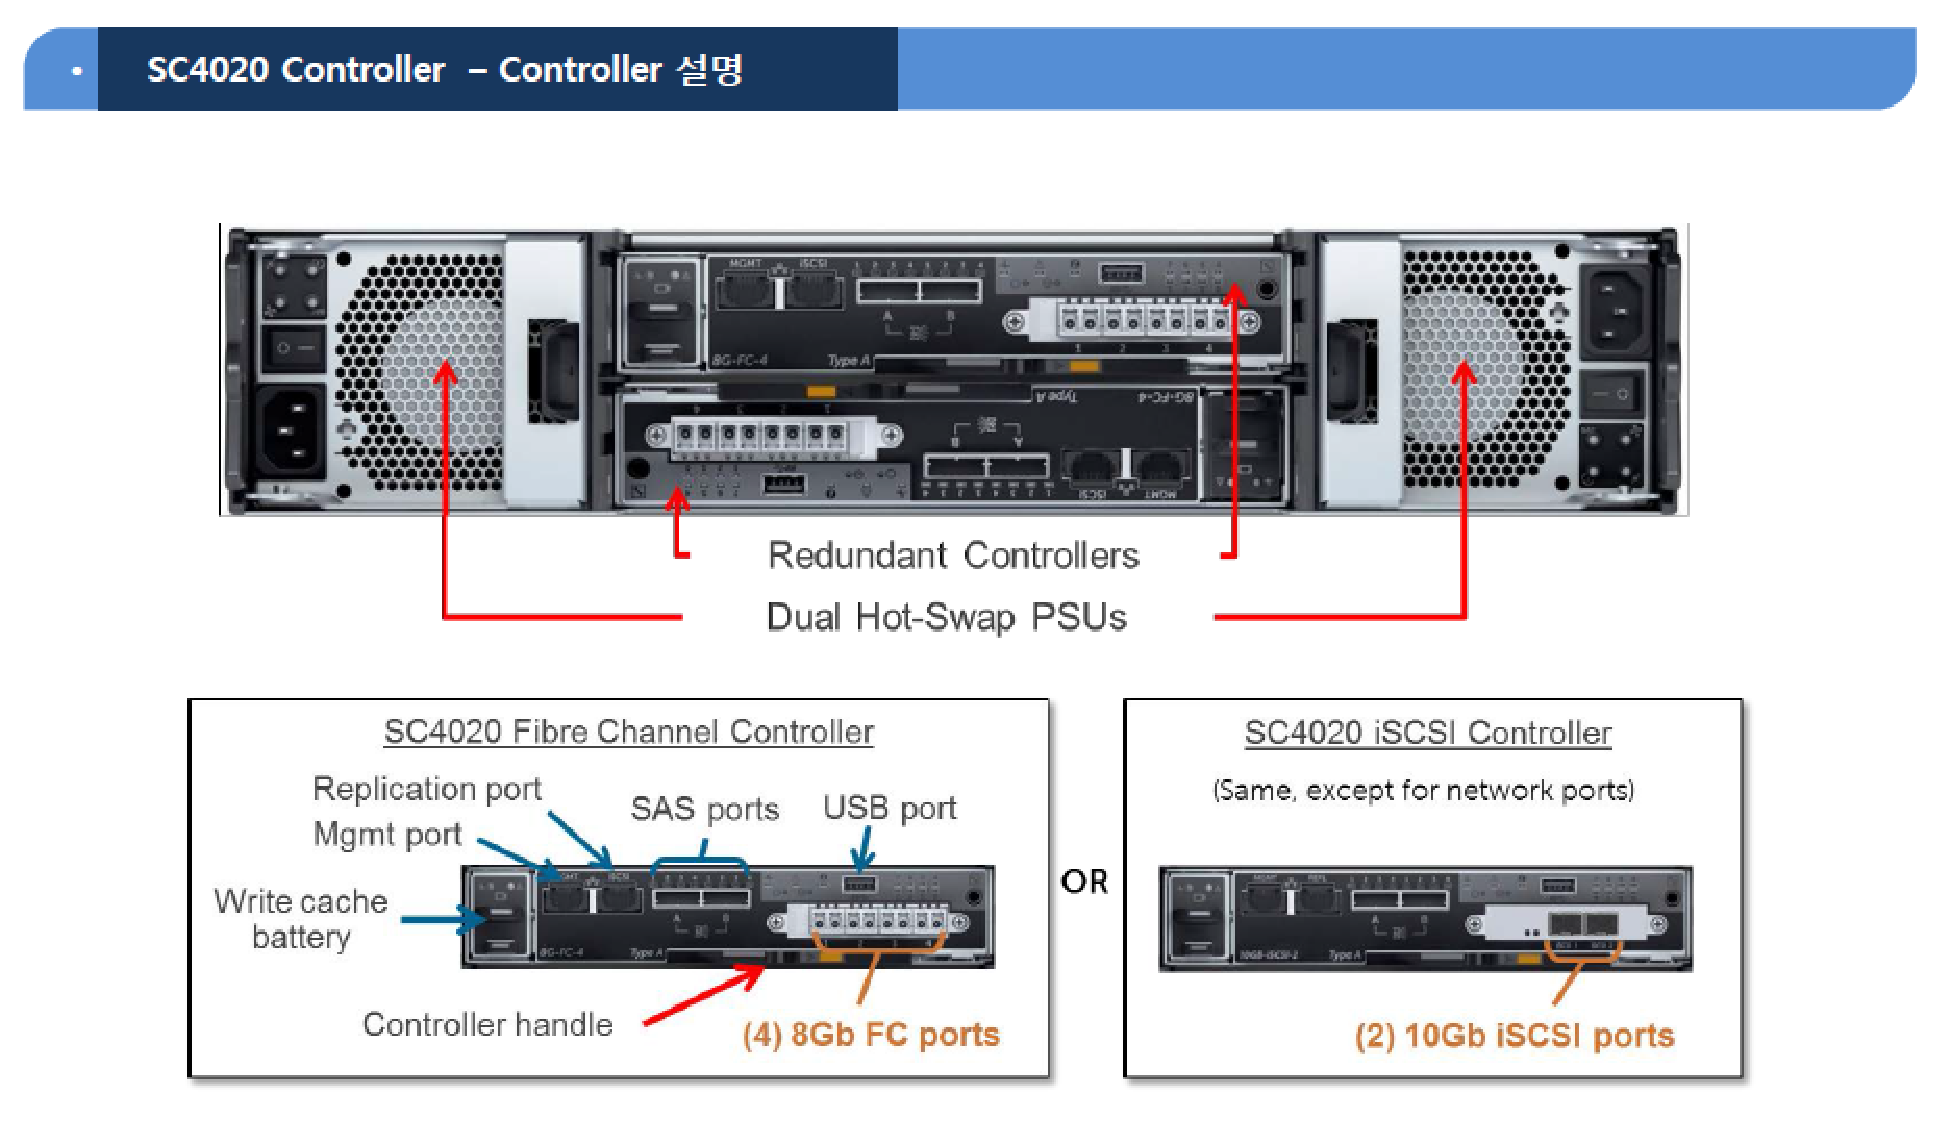
\includegraphics[width=0.85\textwidth]{./images/srfdb_storage_arch_6.eps}
	\caption{SRF Storage Architecture - 6}
	\label{fig:srfdb_arch_6} 
\end{figure}

\begin{figure}[h!]
	\centering
	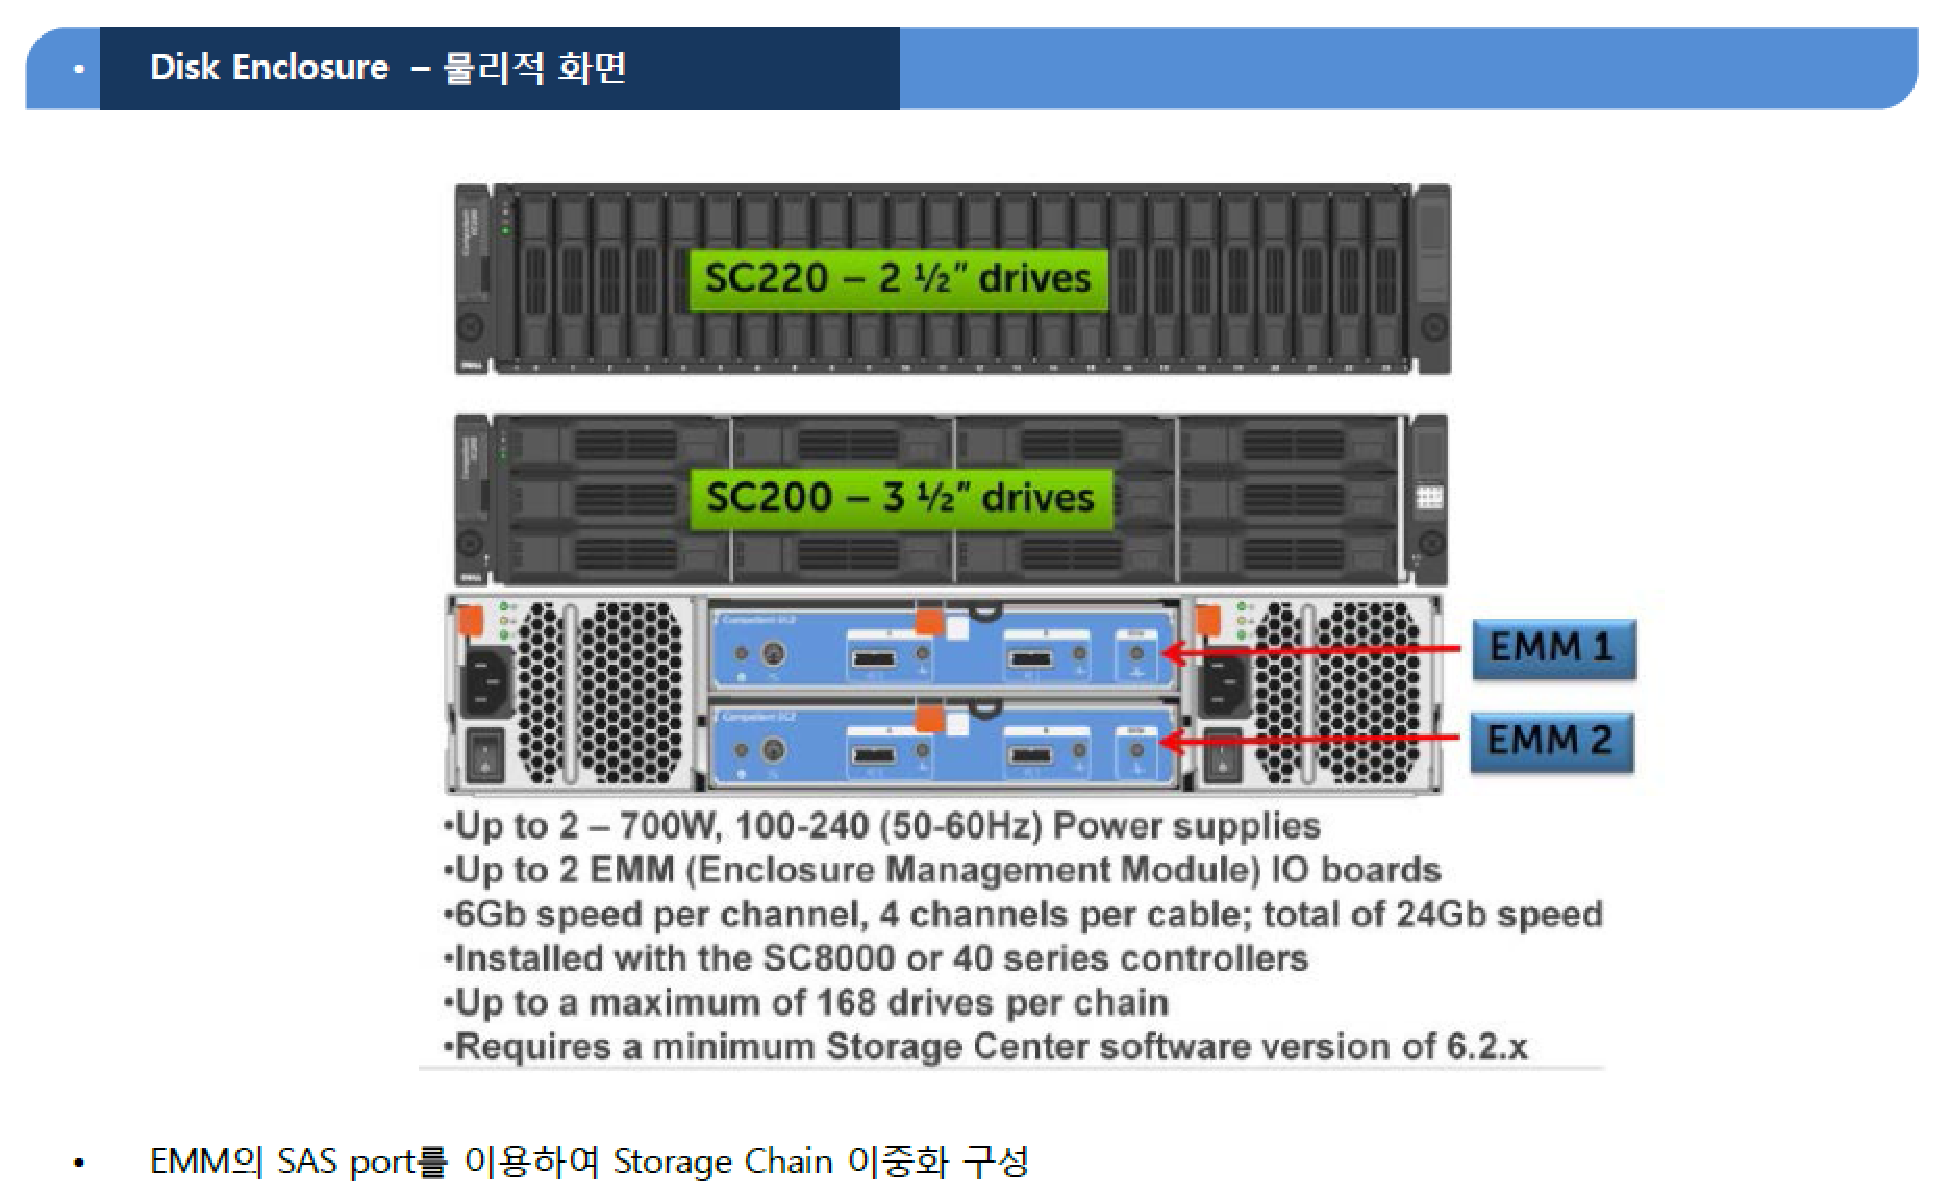
\includegraphics[width=0.85\textwidth]{./images/srfdb_storage_arch_7.eps}
	\caption{SRF Storage Architecture - 7}
	\label{fig:srfdb_arch_7} 
\end{figure}

\begin{figure}[h!]
	\centering
	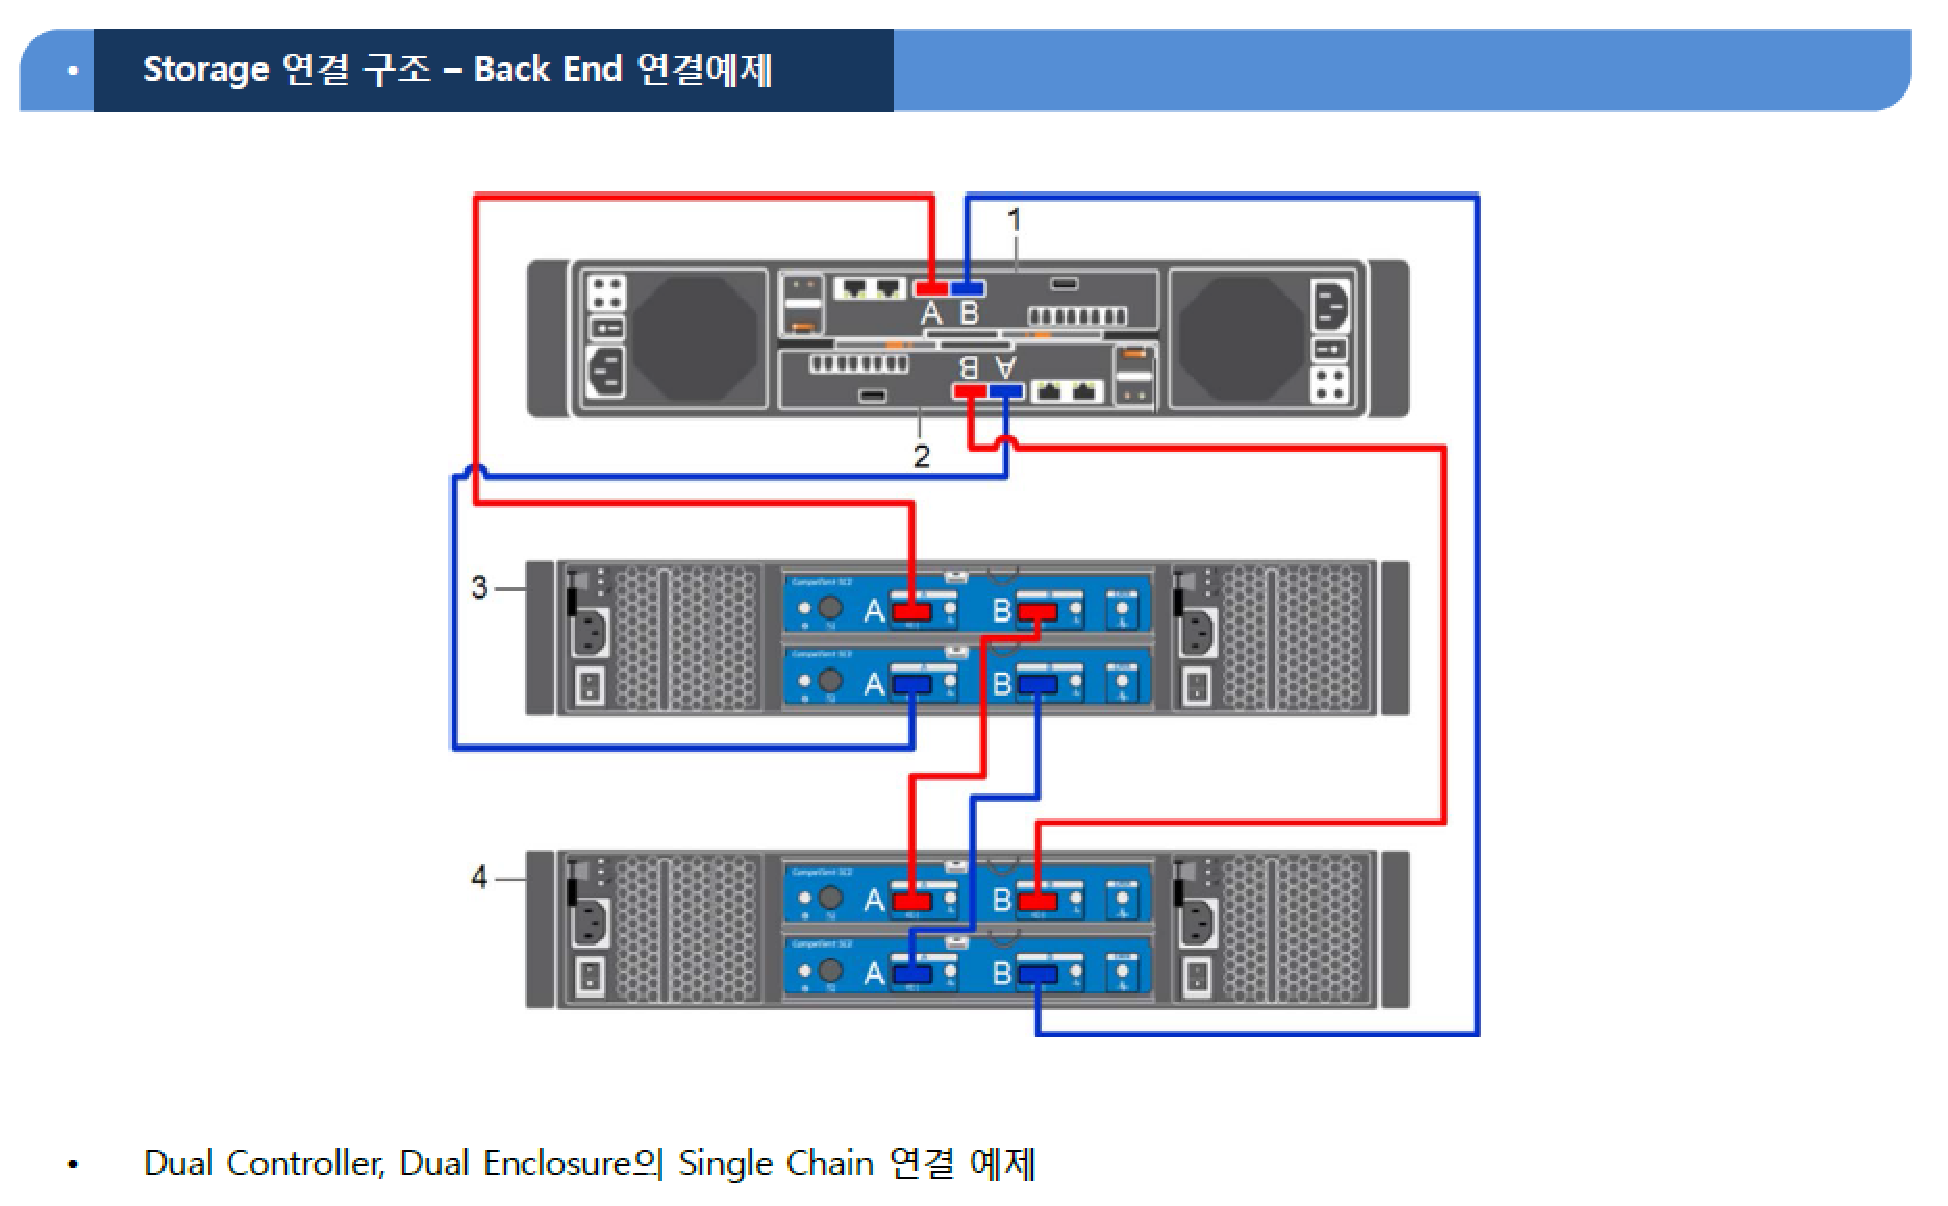
\includegraphics[width=0.85\textwidth]{./images/srfdb_storage_arch_8.eps}
	\caption{SRF Storage Architecture - 8}
	\label{fig:srfdb_arch_8} 
\end{figure}

\clearpage

\section{Storage Management}
\begin{figure}[h!]
	\centering
	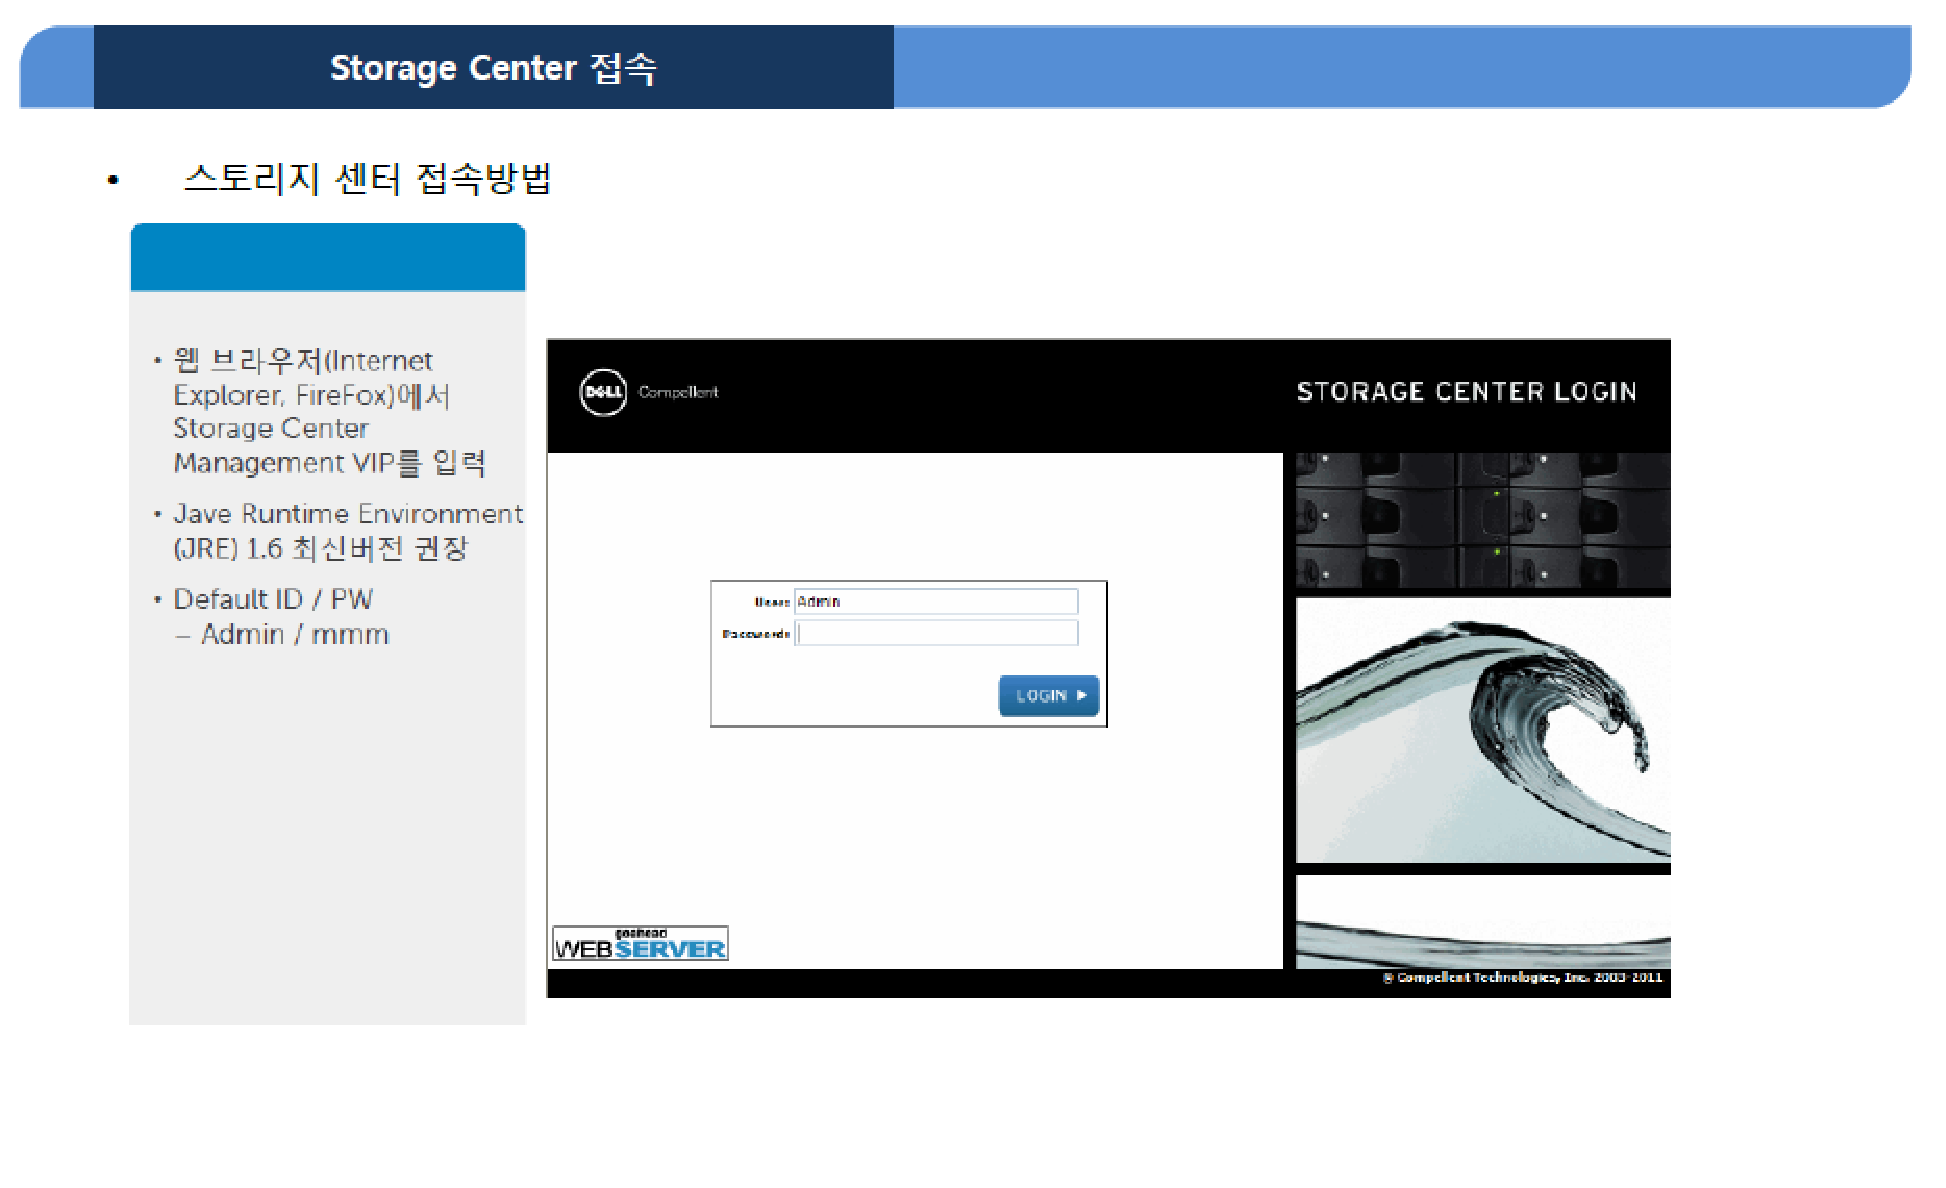
\includegraphics[width=0.85\textwidth]{./images/srfdb_storage_mana_1.eps}
	\caption{SRF Storage Management - 1}
	\label{fig:srfdb_mana_1} 
\end{figure}

\begin{figure}[h!]
	\centering
	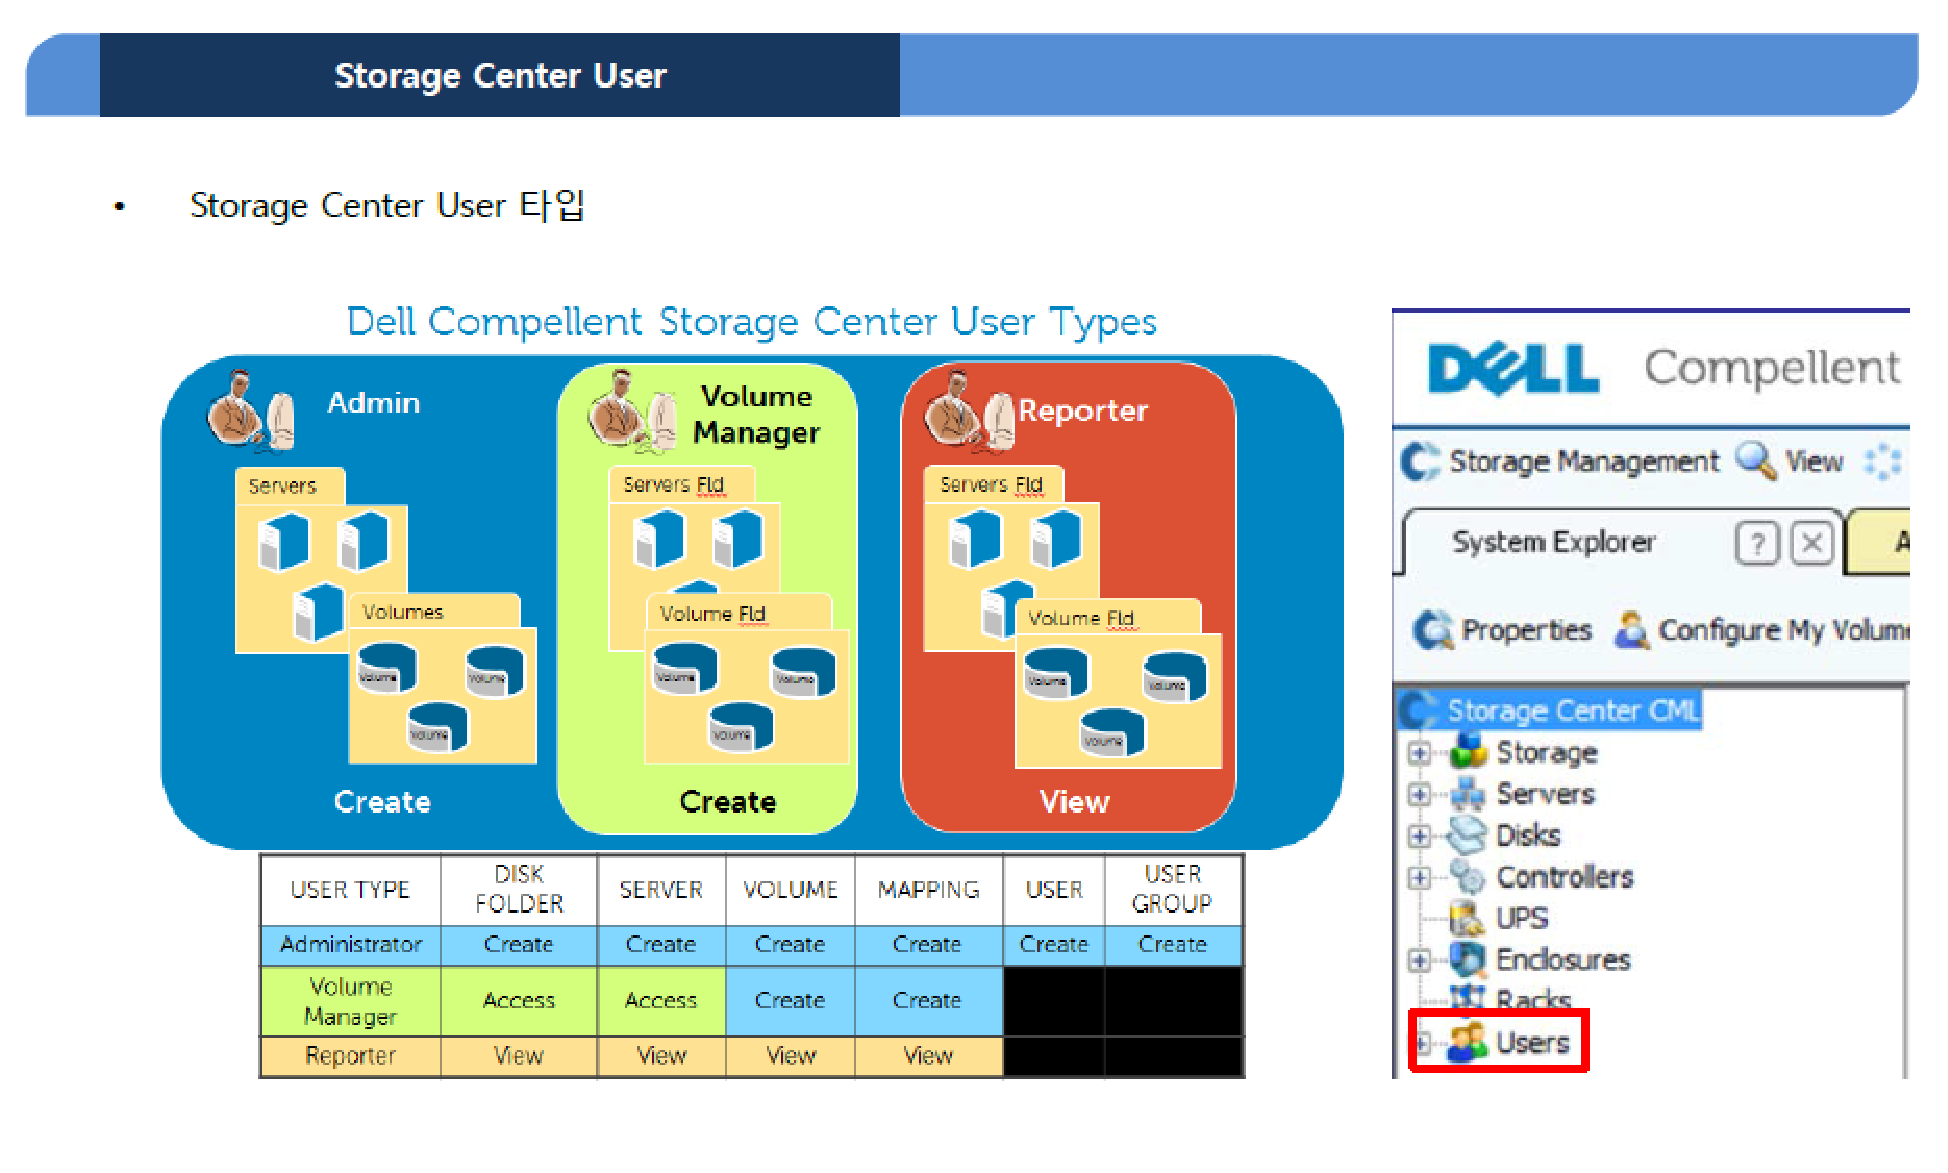
\includegraphics[width=0.85\textwidth]{./images/srfdb_storage_mana_2.eps}
	\caption{SRF Storage Management - 2}
	\label{fig:srfdb_mana_2} 
\end{figure}

\begin{figure}[h!]
	\centering
	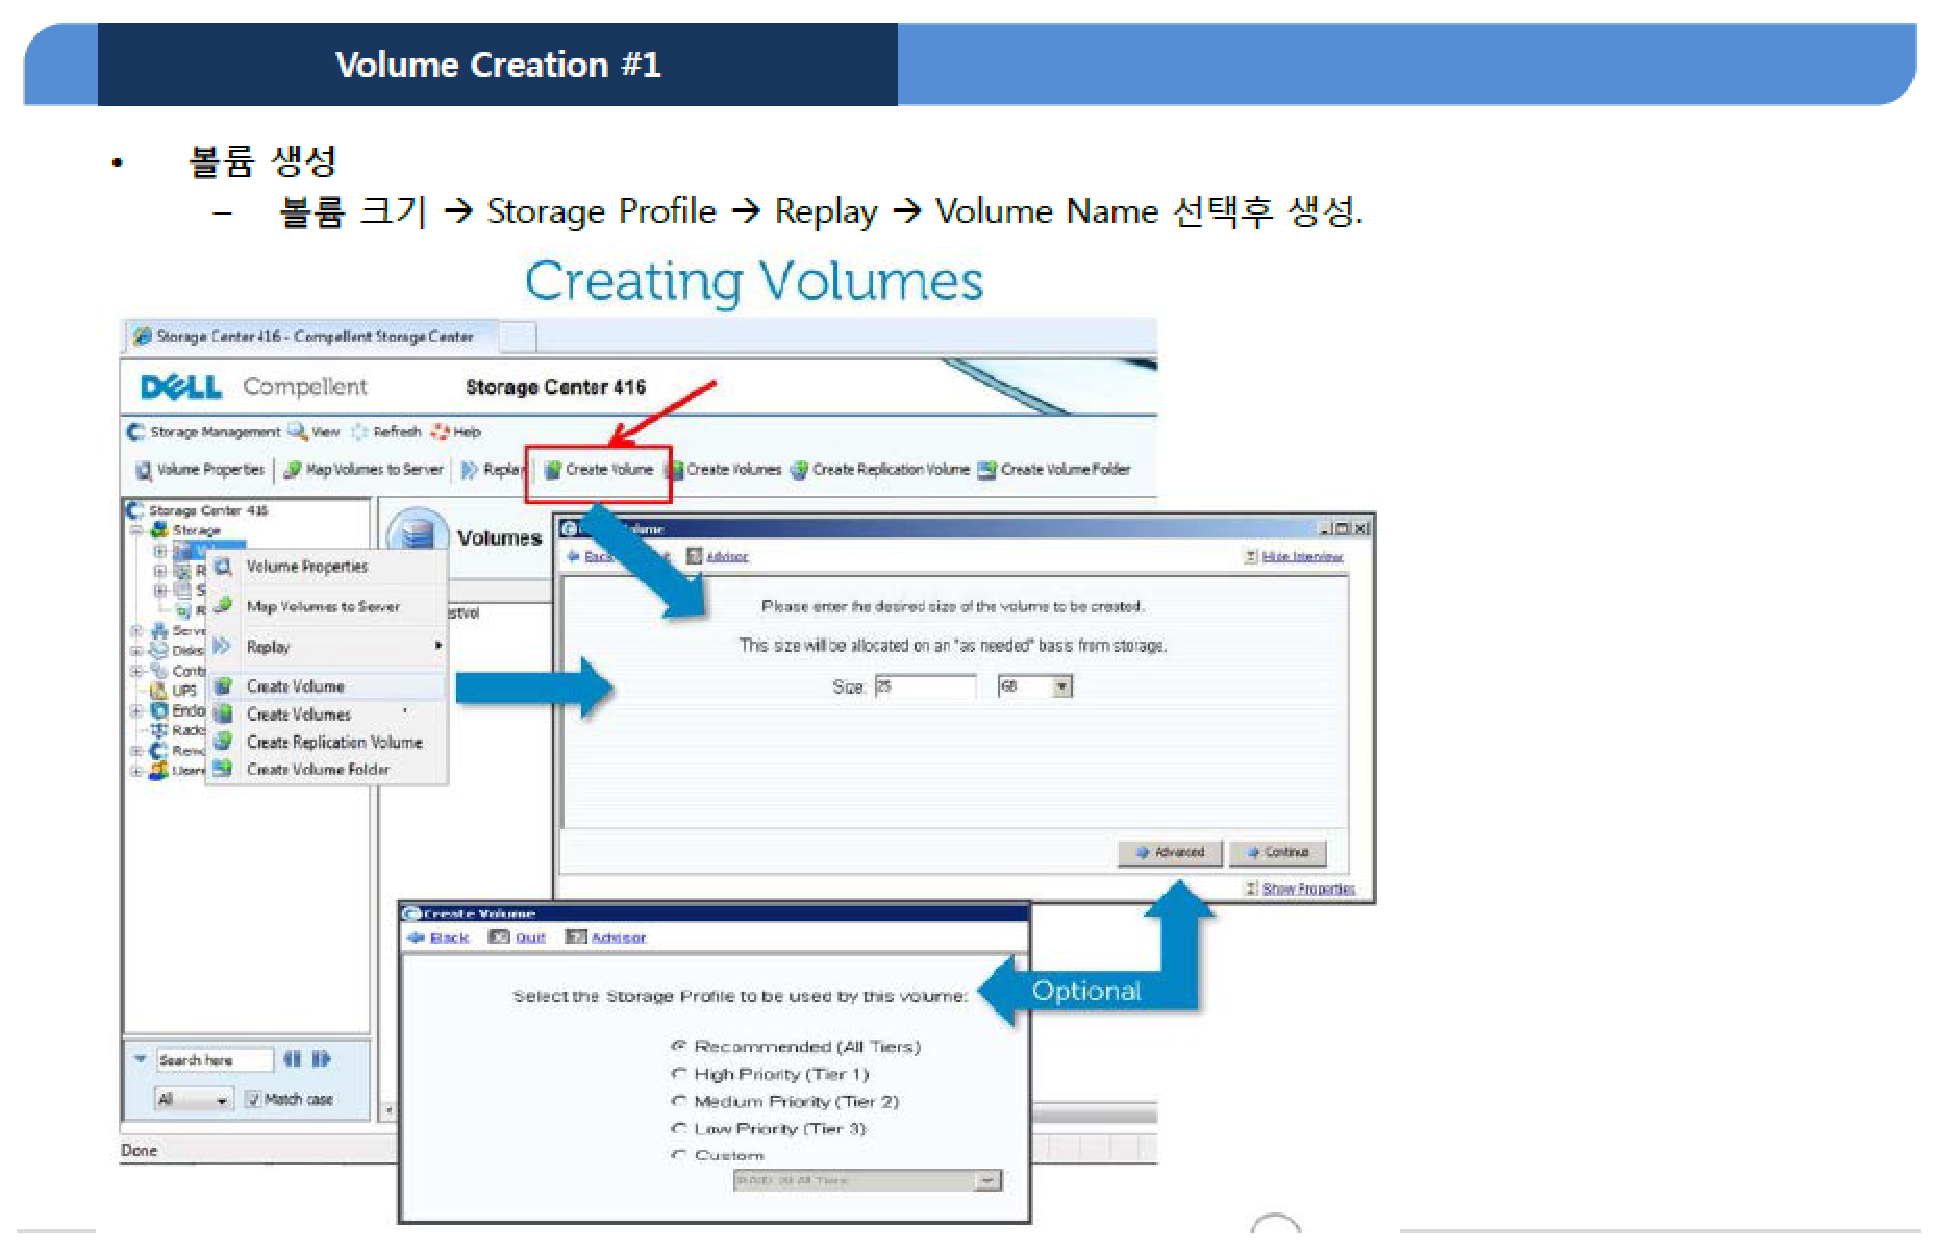
\includegraphics[width=0.85\textwidth]{./images/srfdb_storage_mana_3.eps}
	\caption{SRF Storage Management - 3}
	\label{fig:srfdb_mana_3} 
\end{figure}

\begin{figure}[h!]
	\centering
	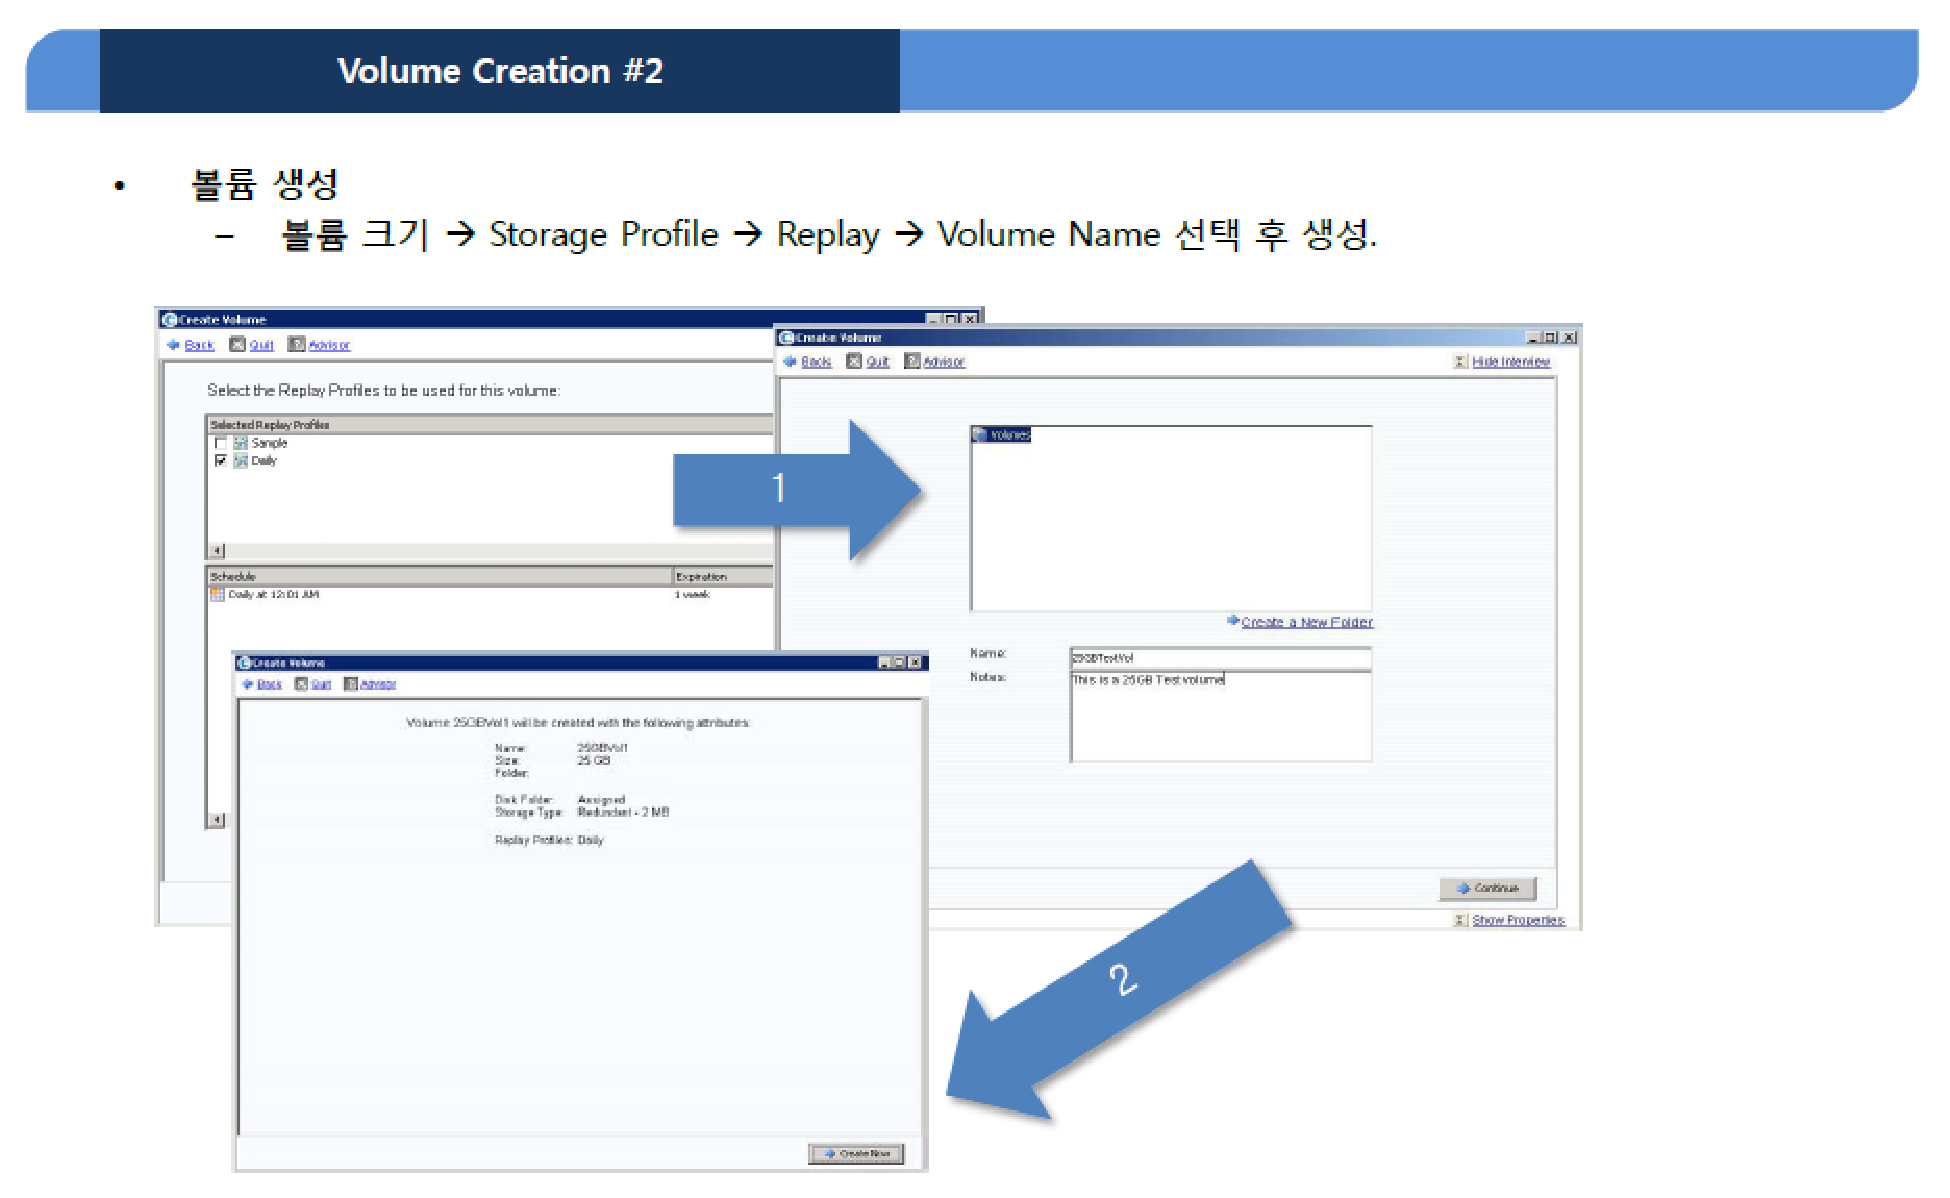
\includegraphics[width=0.85\textwidth]{./images/srfdb_storage_mana_4.eps}
	\caption{SRF Storage Management - 4}
	\label{fig:srfdb_mana_4} 
\end{figure}

\begin{figure}[h!]
	\centering
	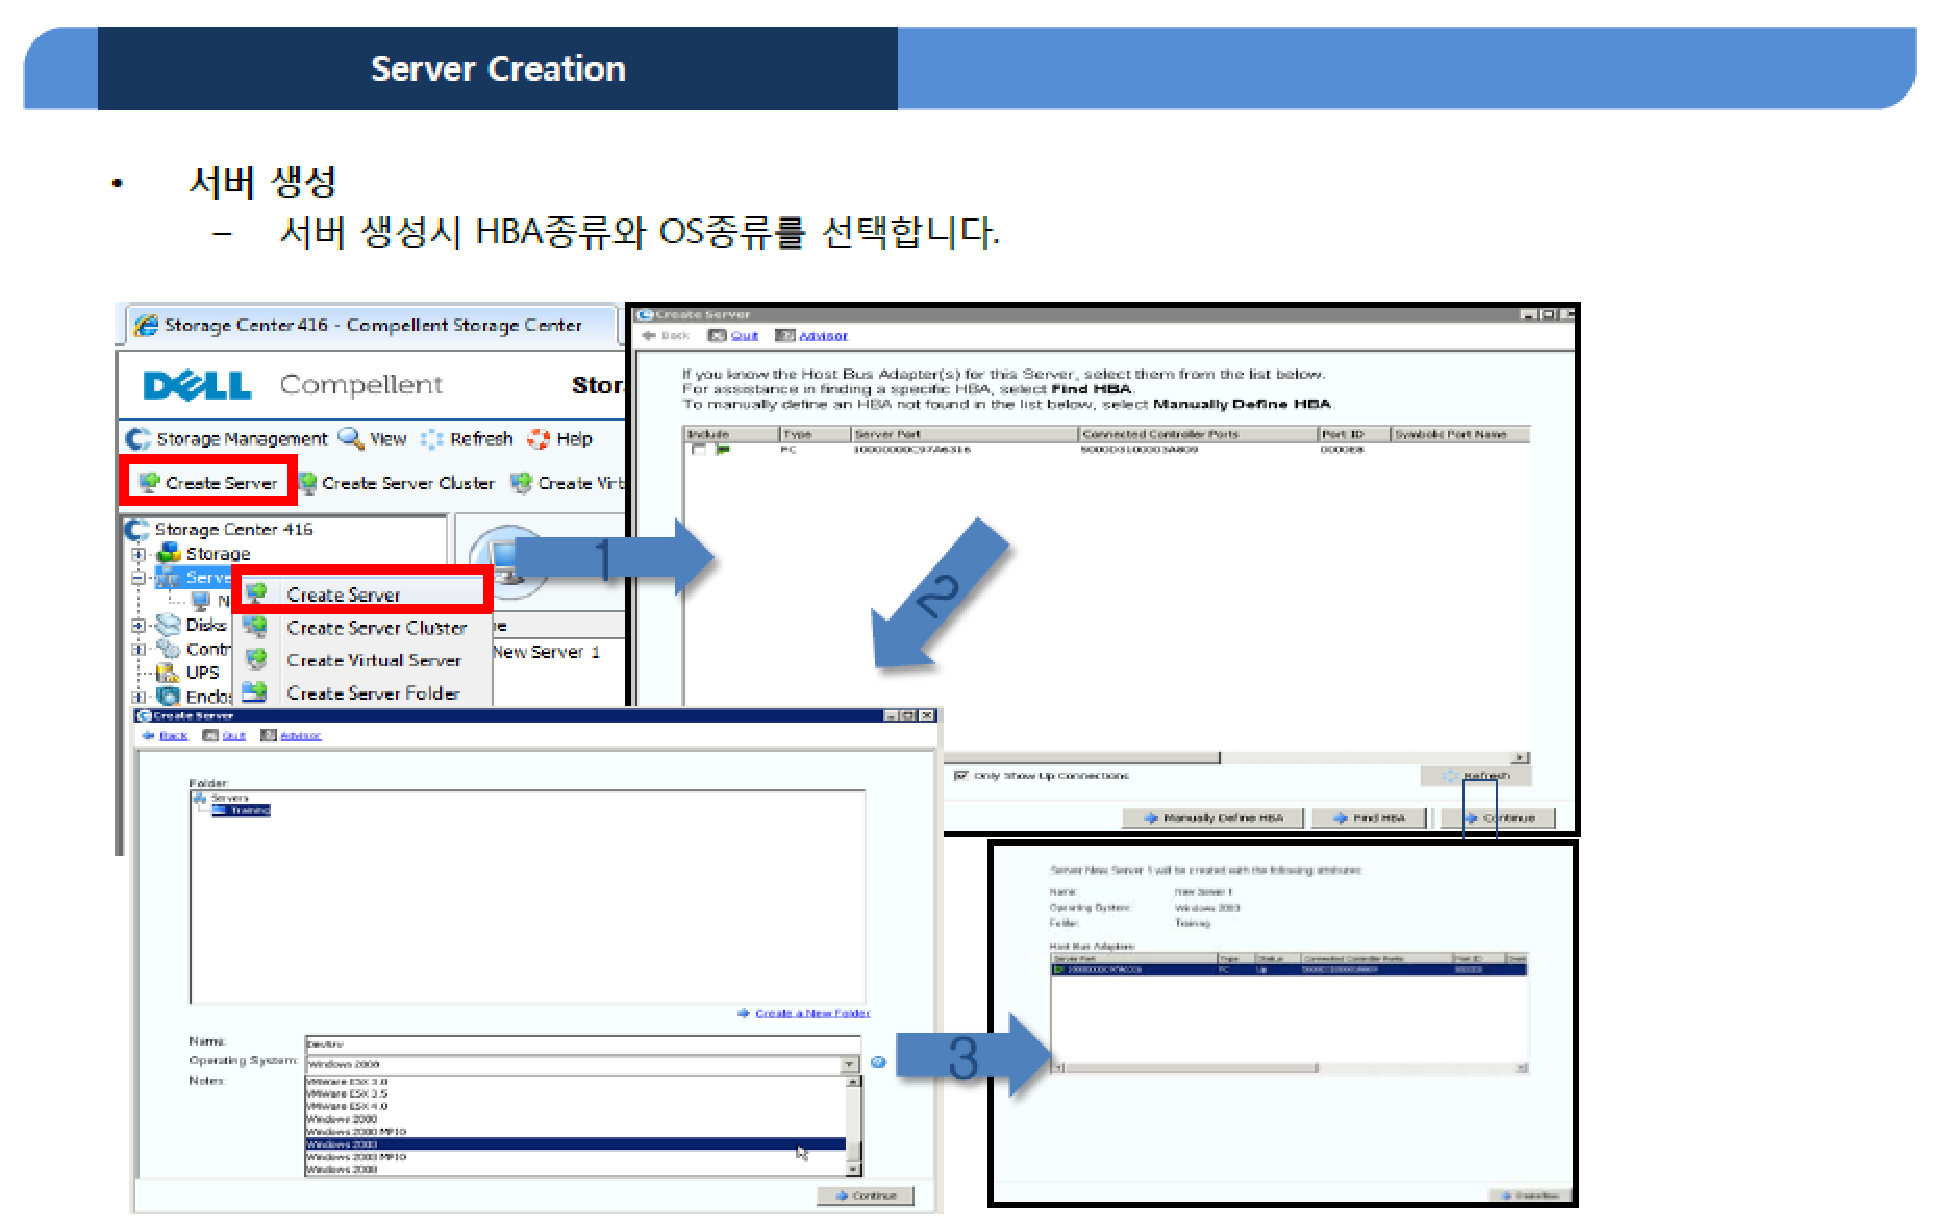
\includegraphics[width=0.85\textwidth]{./images/srfdb_storage_mana_5.eps}
	\caption{SRF Storage Management - 5}
	\label{fig:srfdb_mana_5} 
\end{figure}

\begin{figure}[h!]
	\centering
	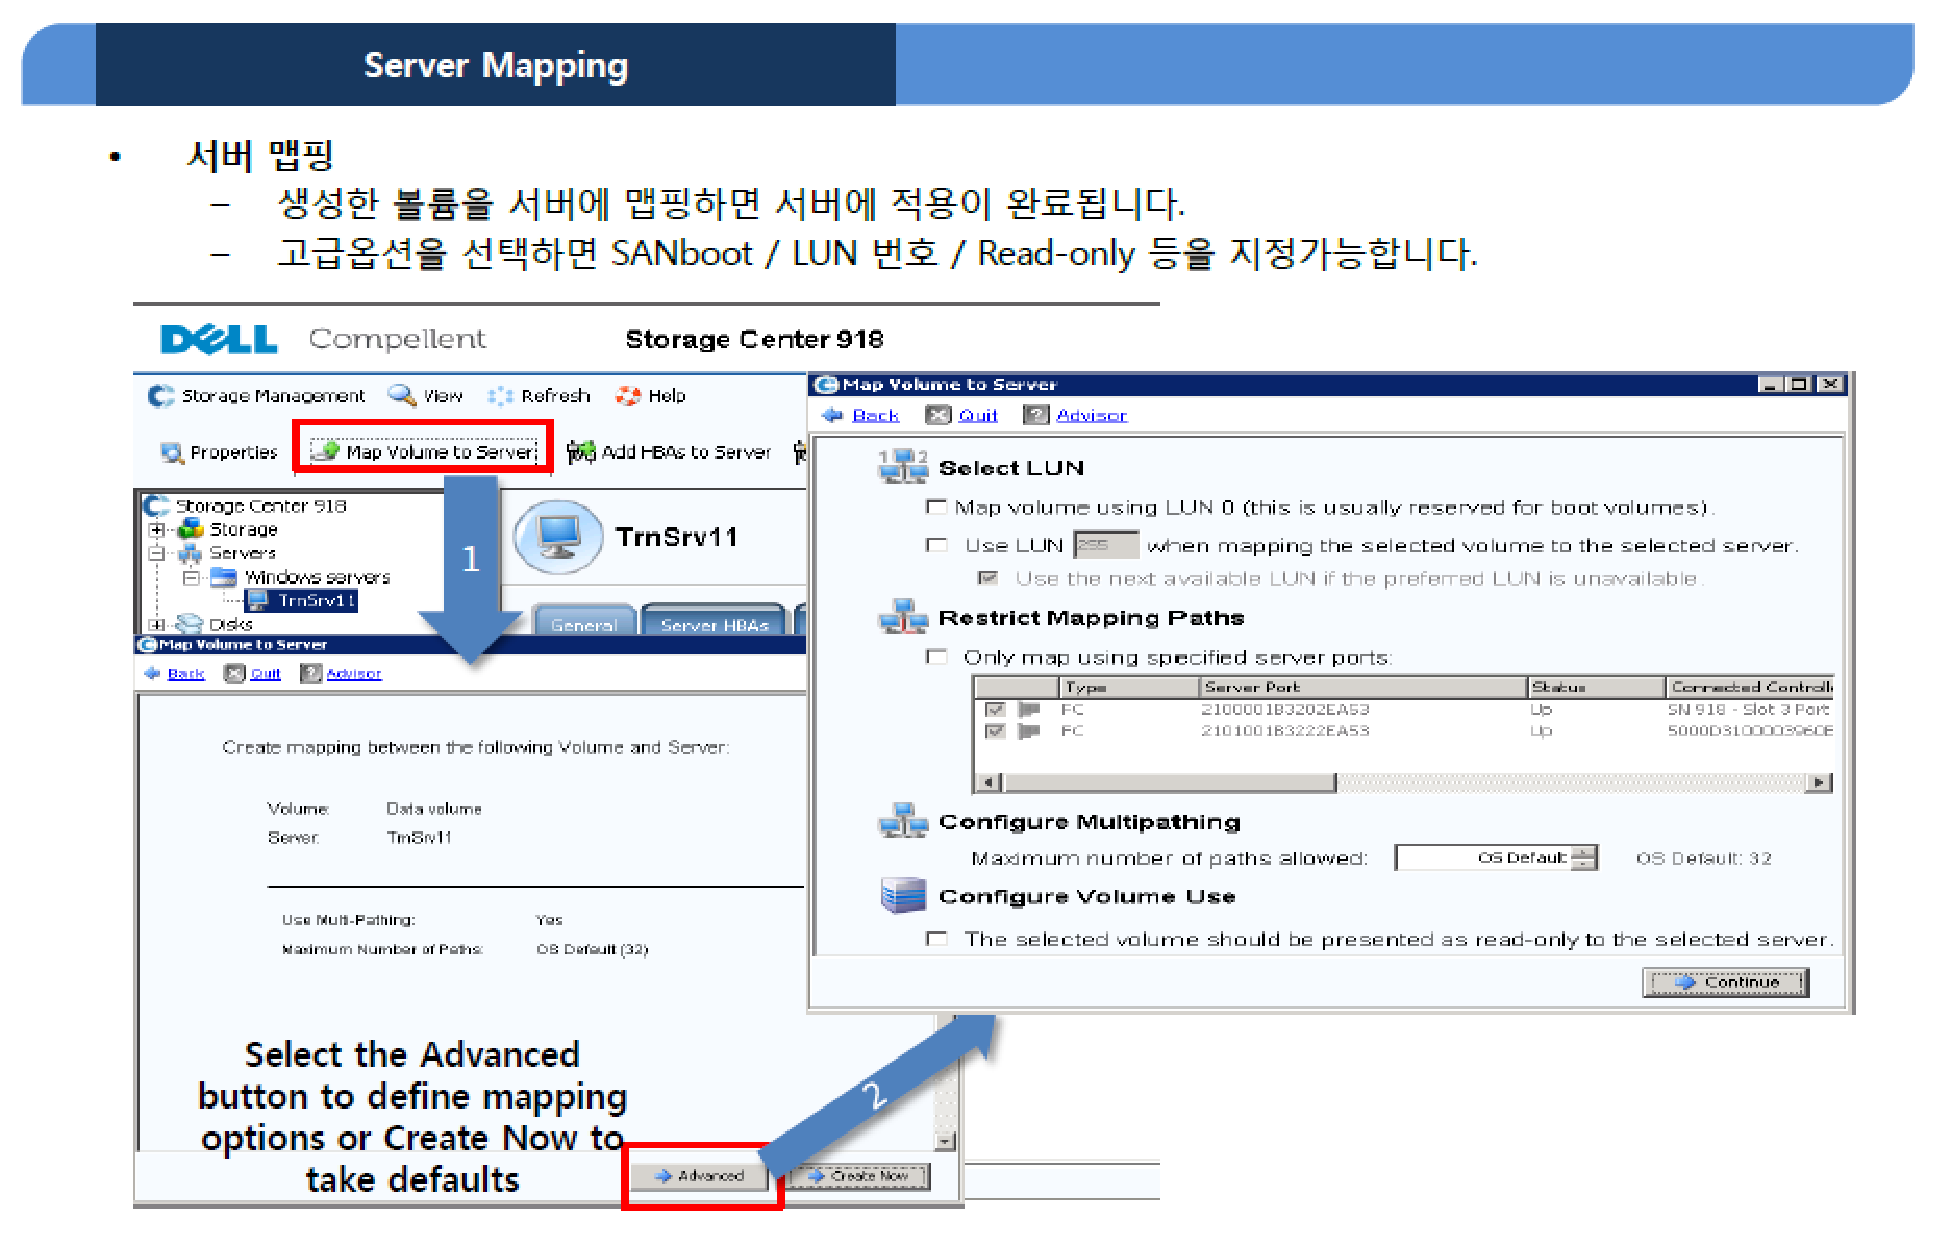
\includegraphics[width=0.85\textwidth]{./images/srfdb_storage_mana_6.eps}
	\caption{SRF Storage Management - 6}
	\label{fig:srfdb_mana_6} 
\end{figure}

\begin{figure}[h!]
	\centering
	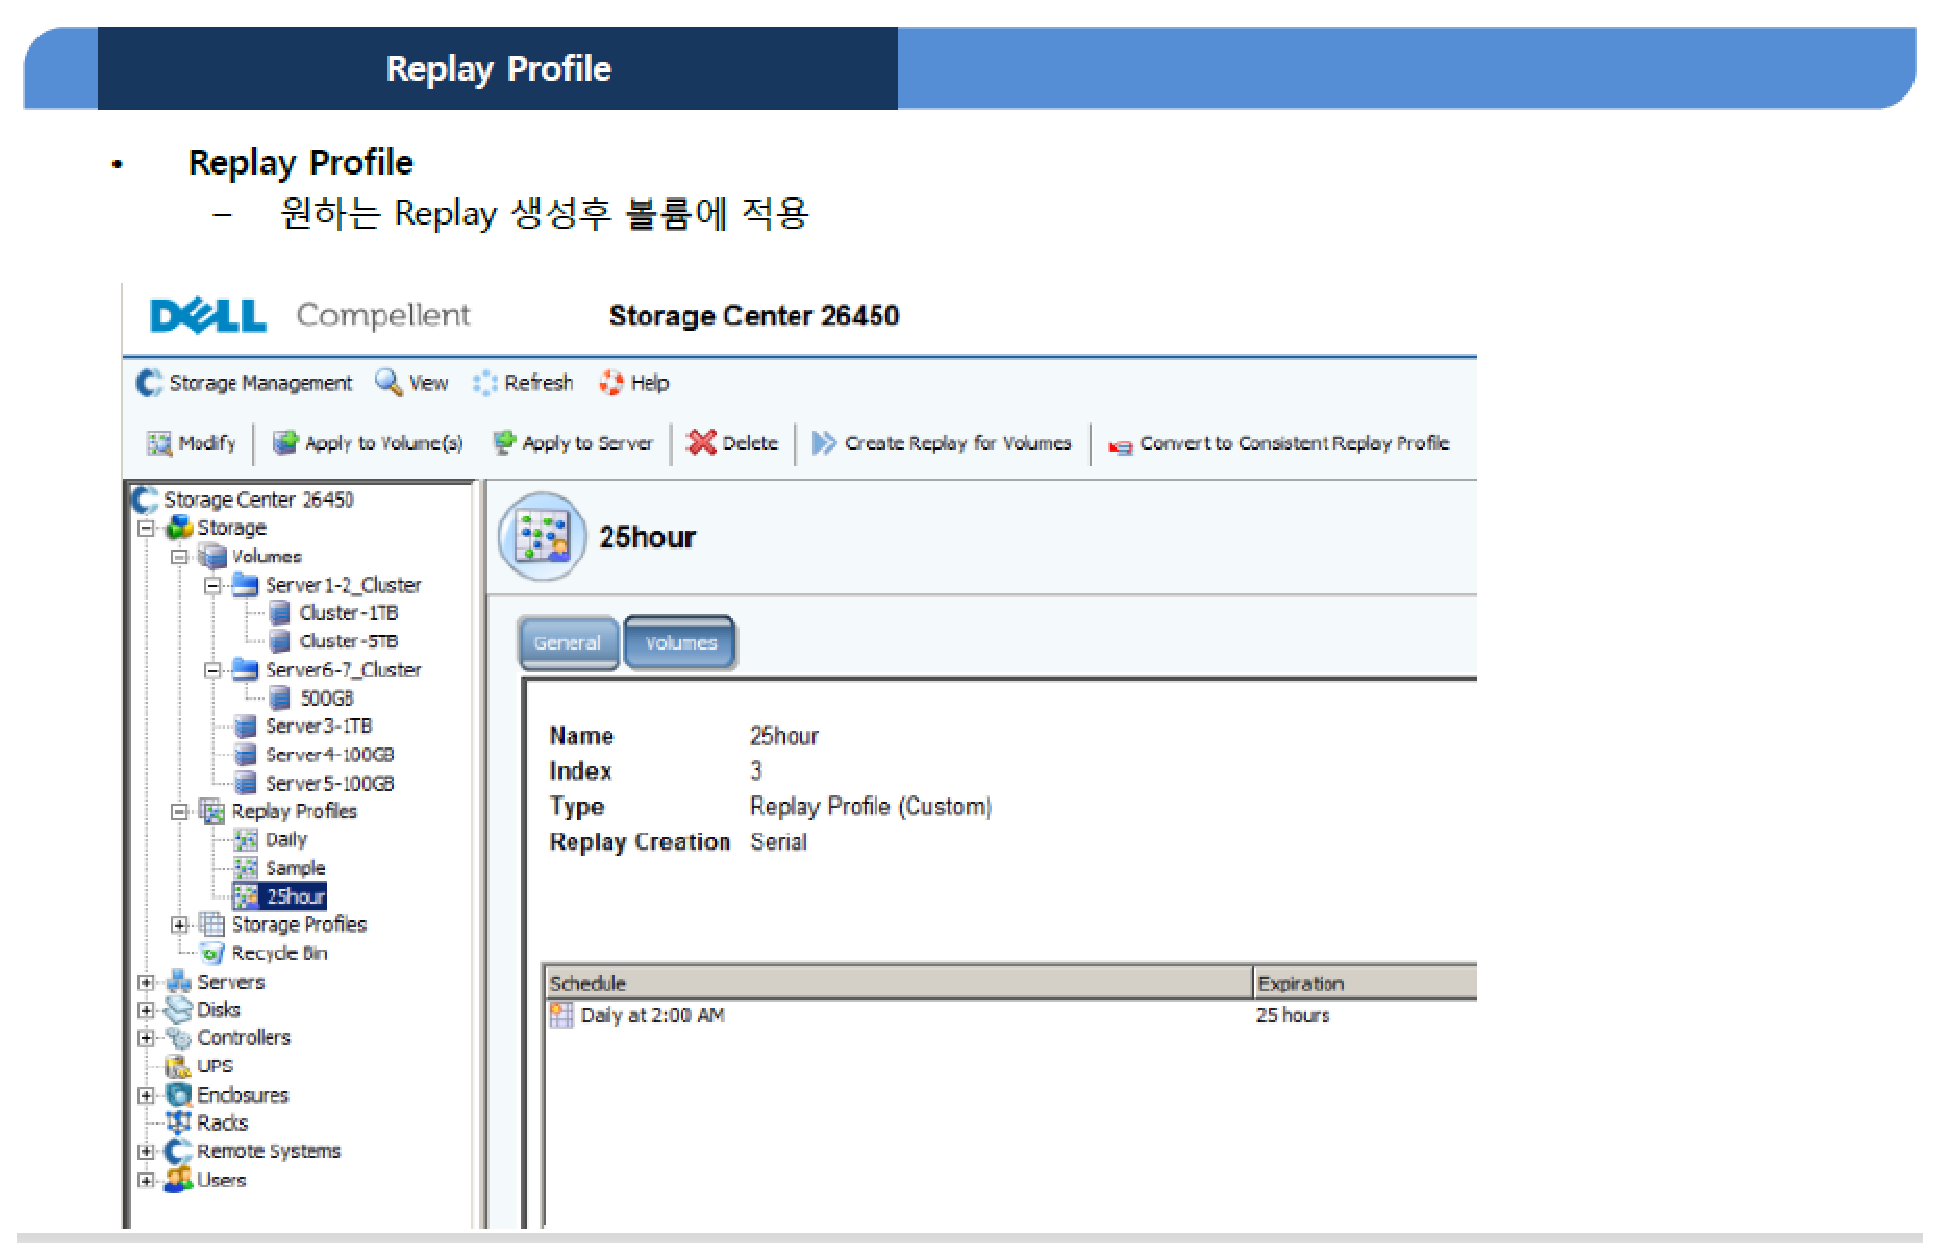
\includegraphics[width=0.85\textwidth]{./images/srfdb_storage_mana_7.eps}
	\caption{SRF Storage Management - 7}
	\label{fig:srfdb_mana_7} 
\end{figure}

\begin{figure}[h!]
	\centering
	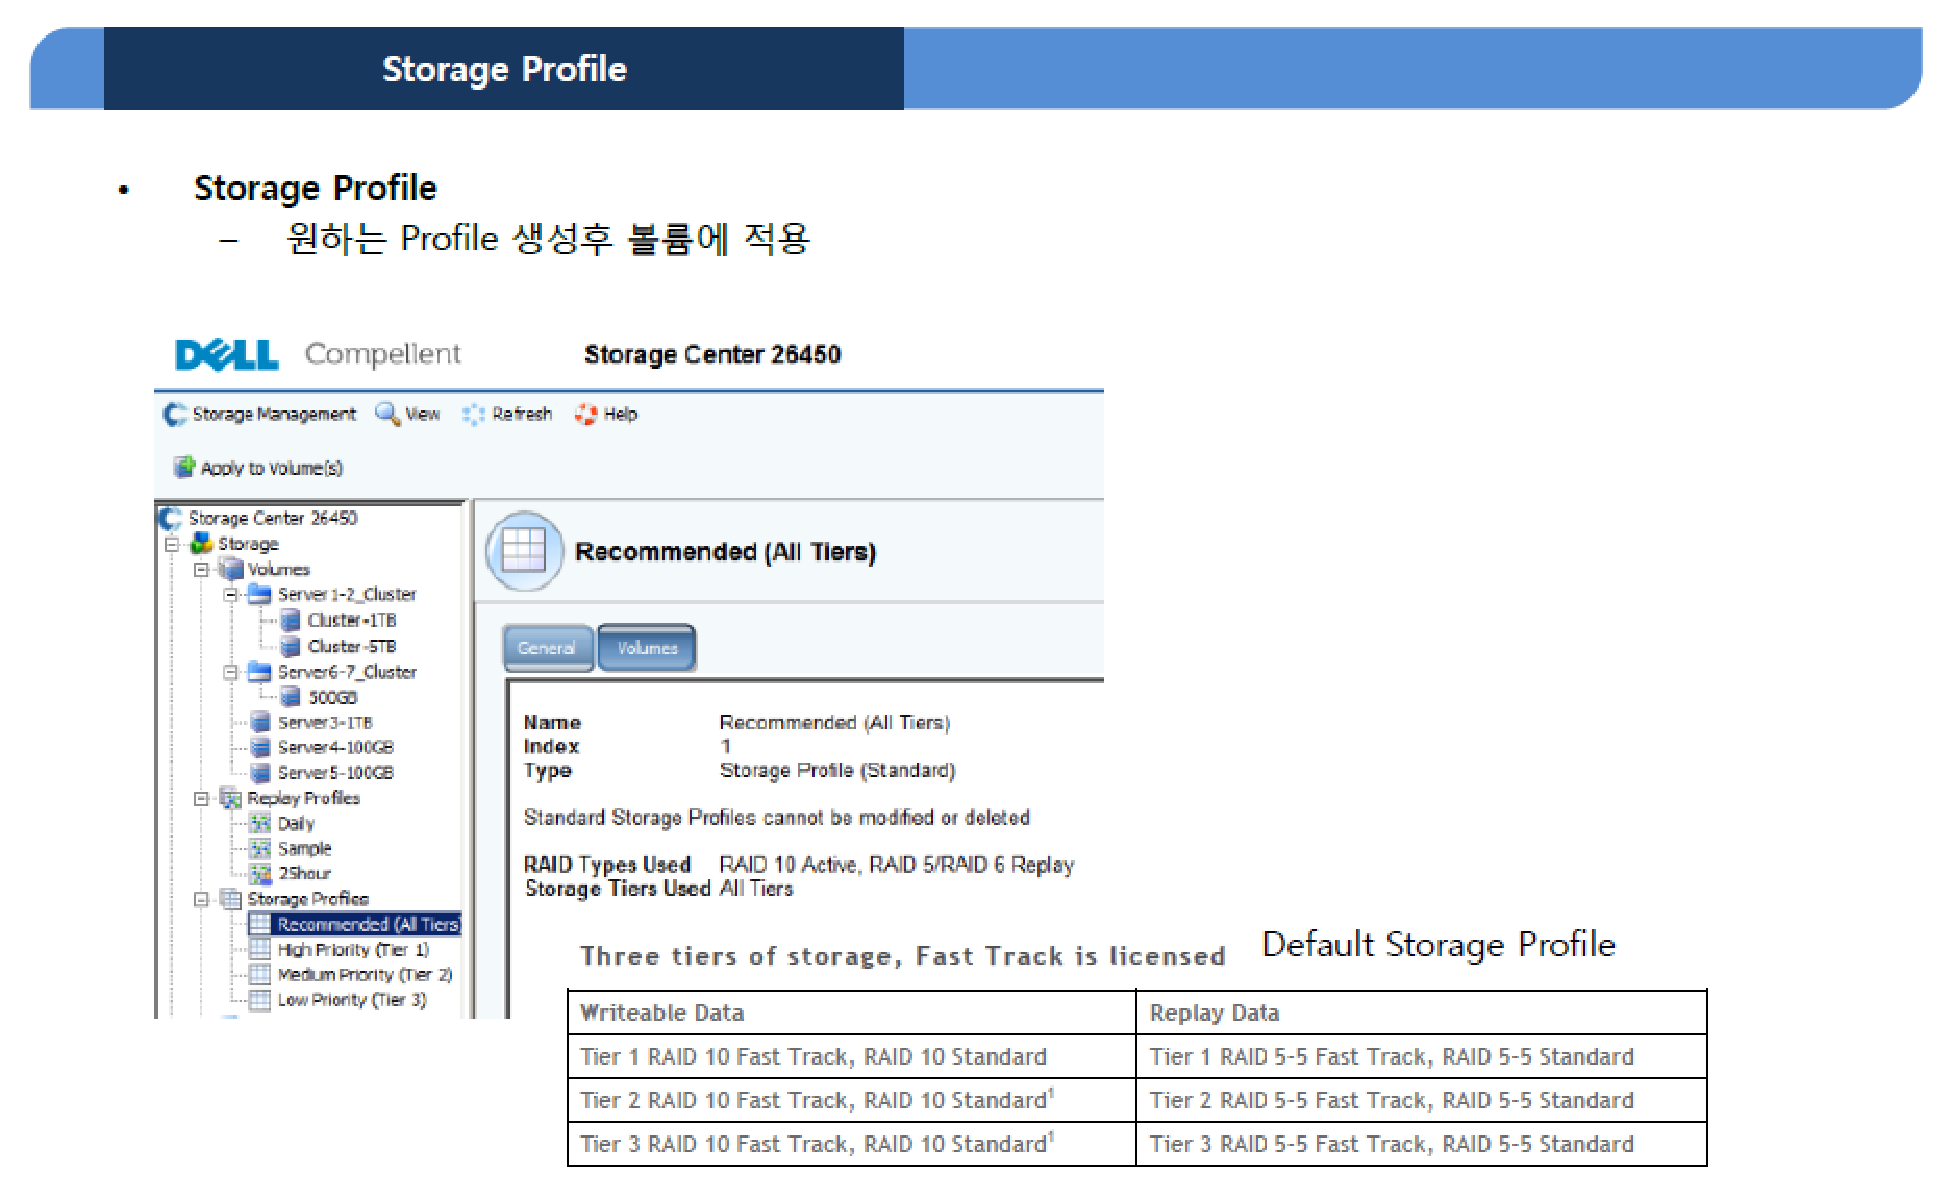
\includegraphics[width=0.85\textwidth]{./images/srfdb_storage_mana_8.eps}
	\caption{SRF Storage Management - 8}
	\label{fig:srfdb_mana_8} 
\end{figure}

\begin{figure}[h!]
	\centering
	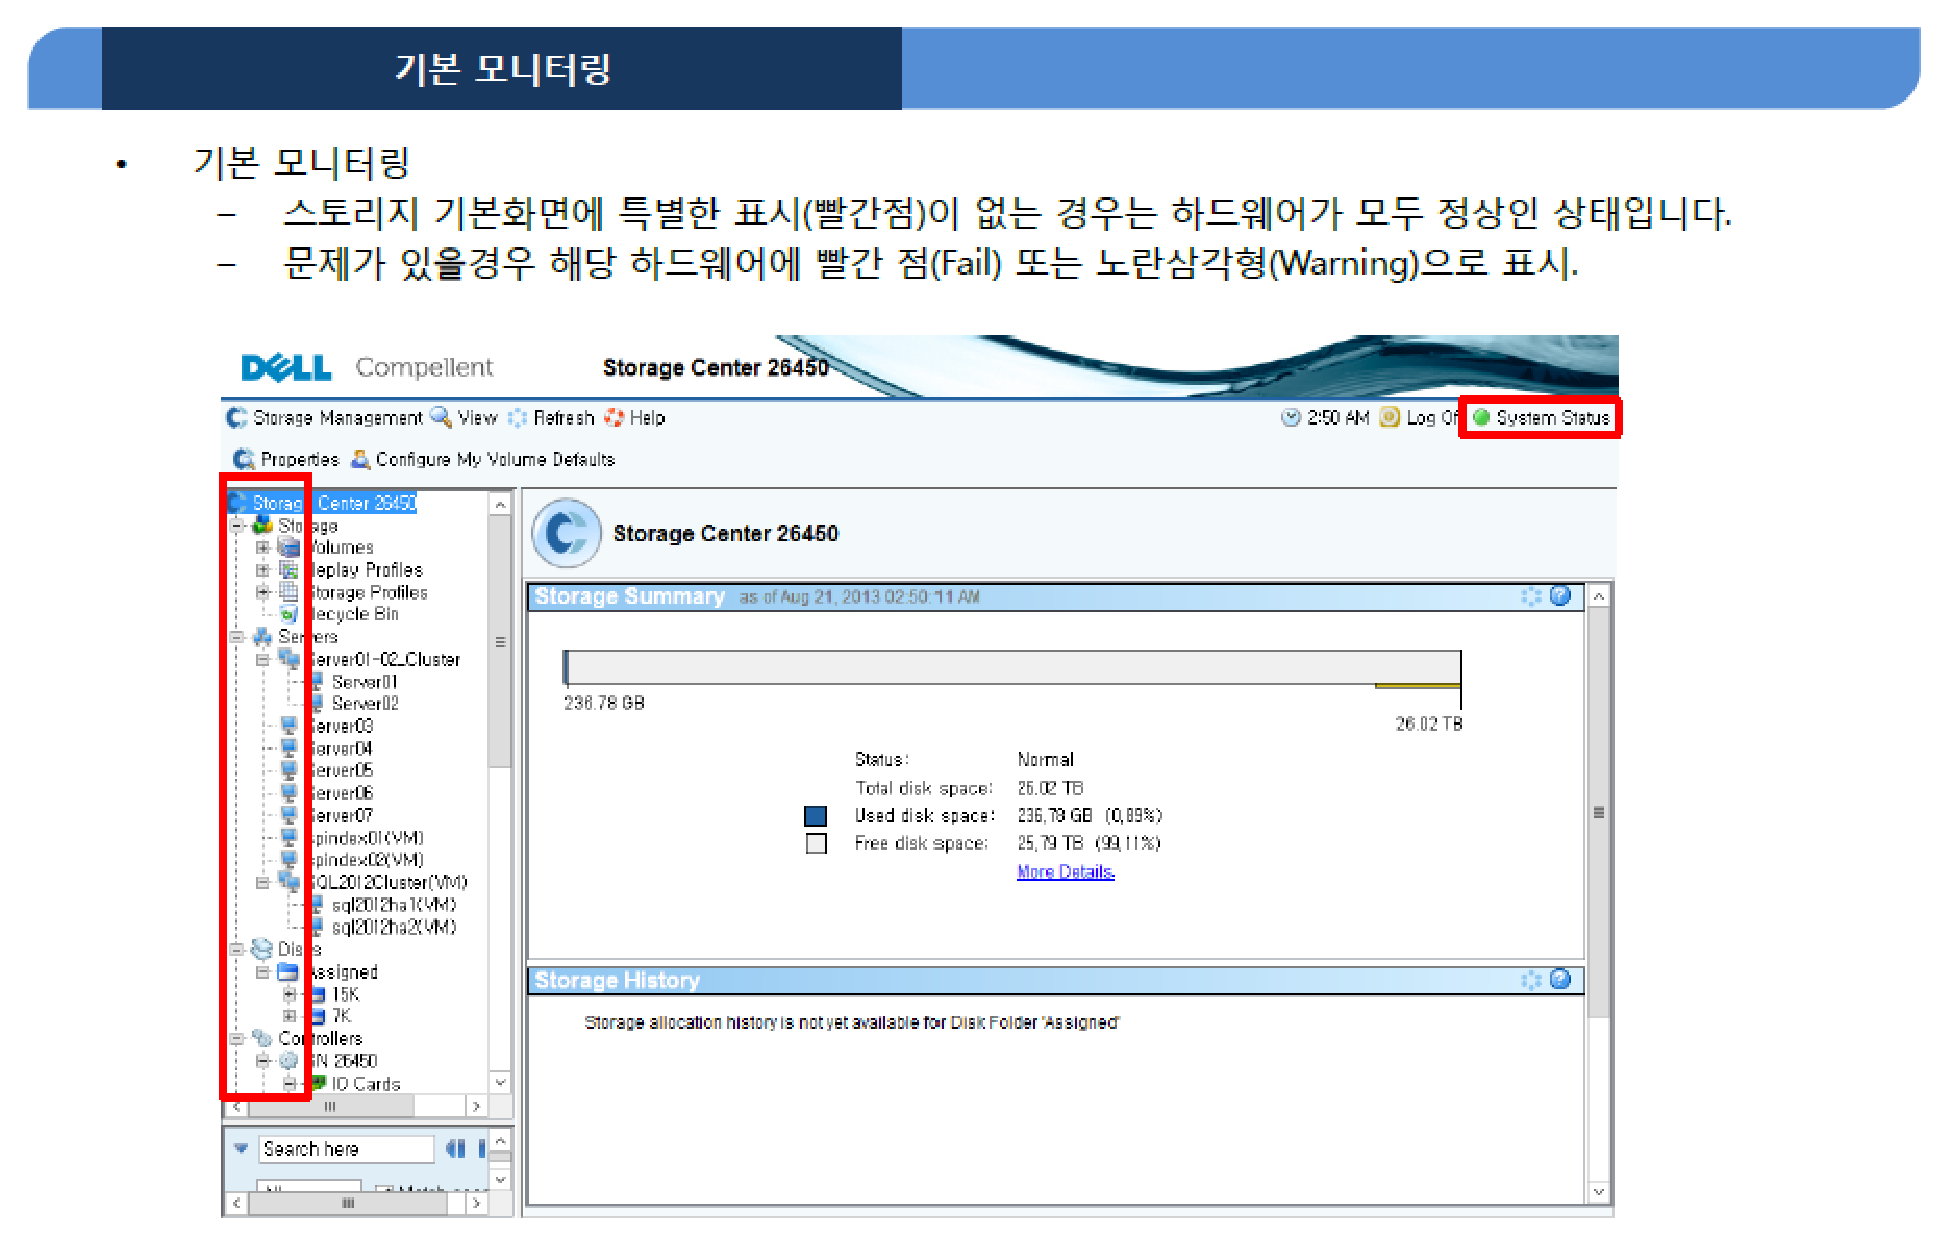
\includegraphics[width=0.85\textwidth]{./images/srfdb_storage_mana_9.eps}
	\caption{SRF Storage Management - 9}
	\label{fig:srfdb_mana_9} 
\end{figure}

\begin{figure}[h!]
	\centering
	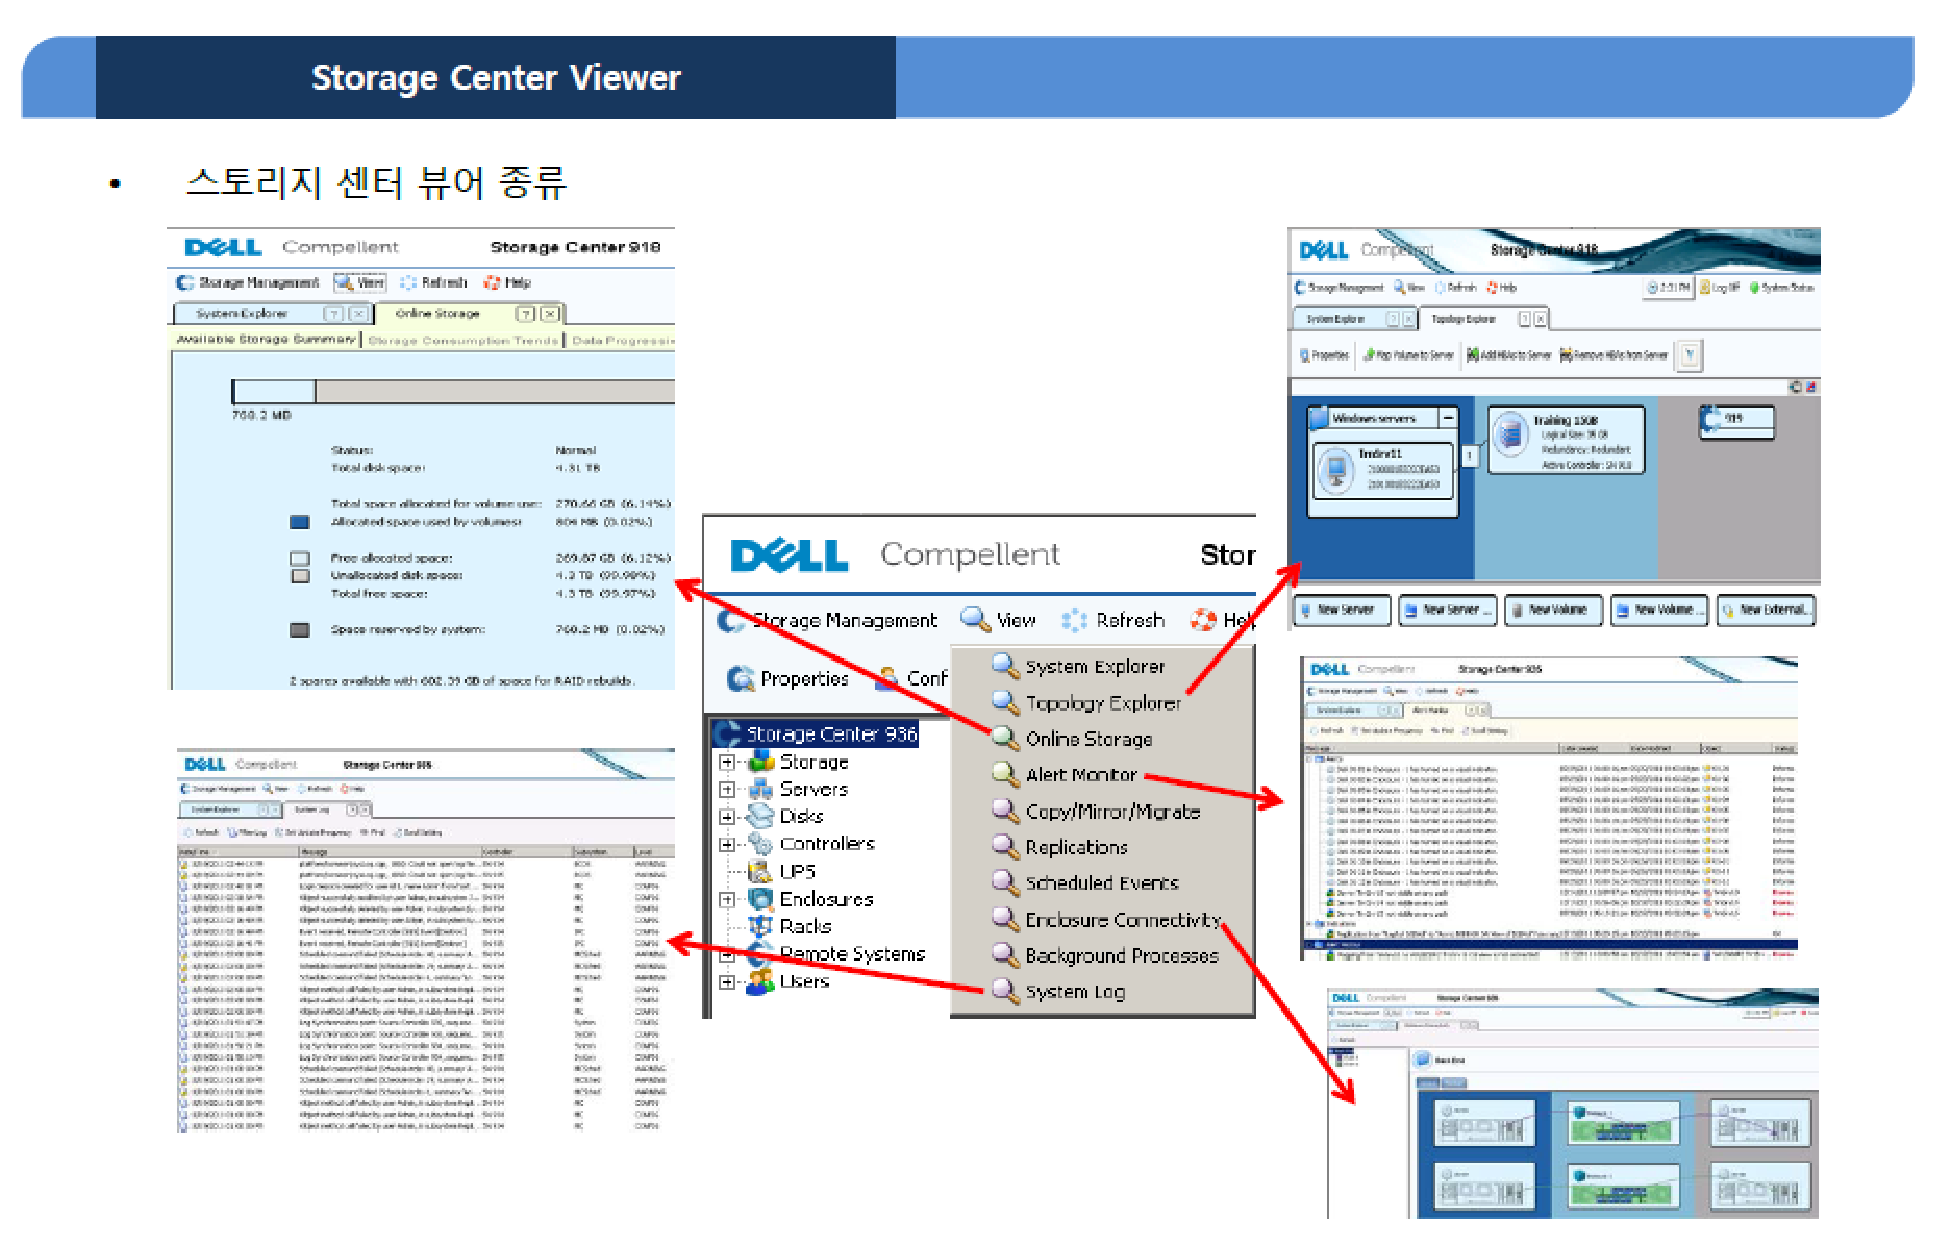
\includegraphics[width=0.85\textwidth]{./images/srfdb_storage_mana_10.eps}
	\caption{SRF Storage Management - 10}
	\label{fig:srfdb_mana_10} 
\end{figure}

\begin{figure}[h!]
	\centering
	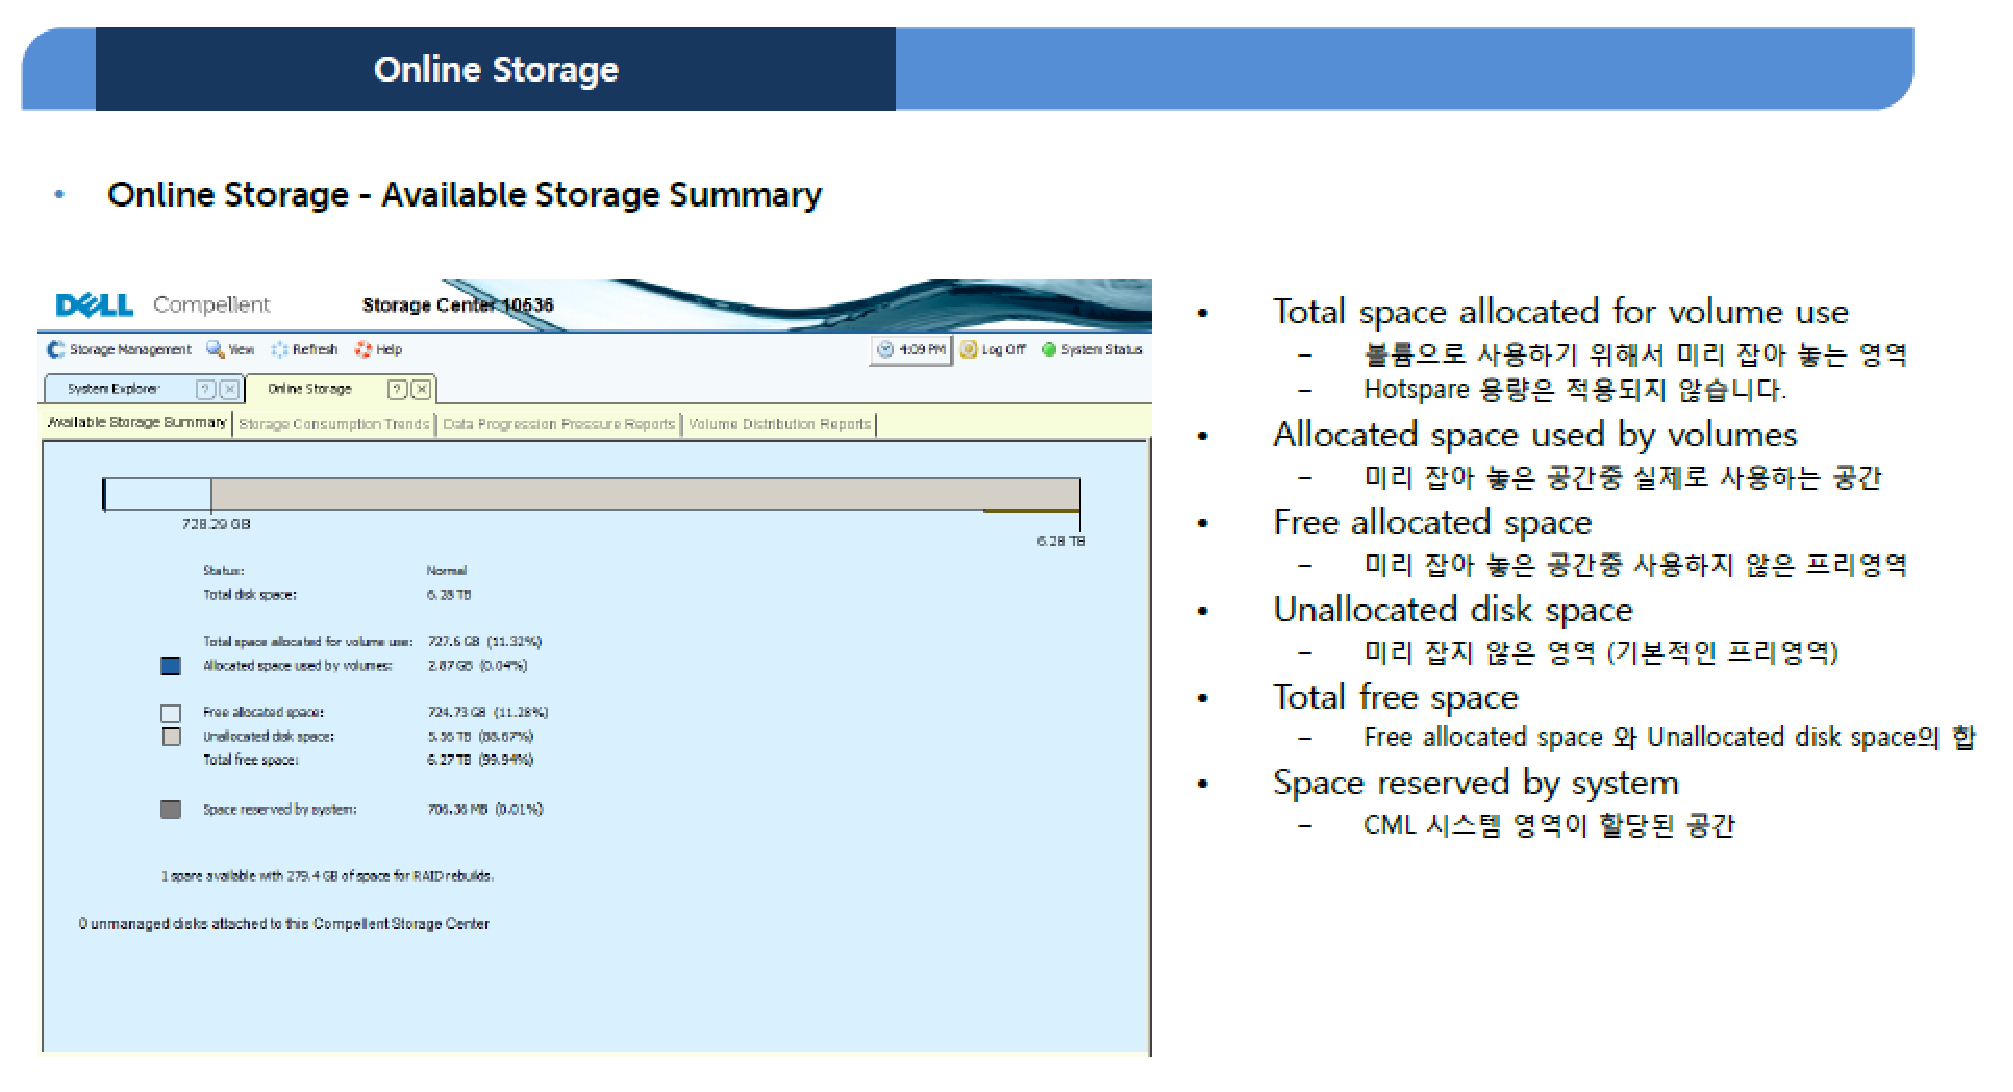
\includegraphics[width=0.85\textwidth]{./images/srfdb_storage_mana_11.eps}
	\caption{SRF Storage Management - 11}
	\label{fig:srfdb_mana_11} 
\end{figure}

\begin{figure}[h!]
	\centering
	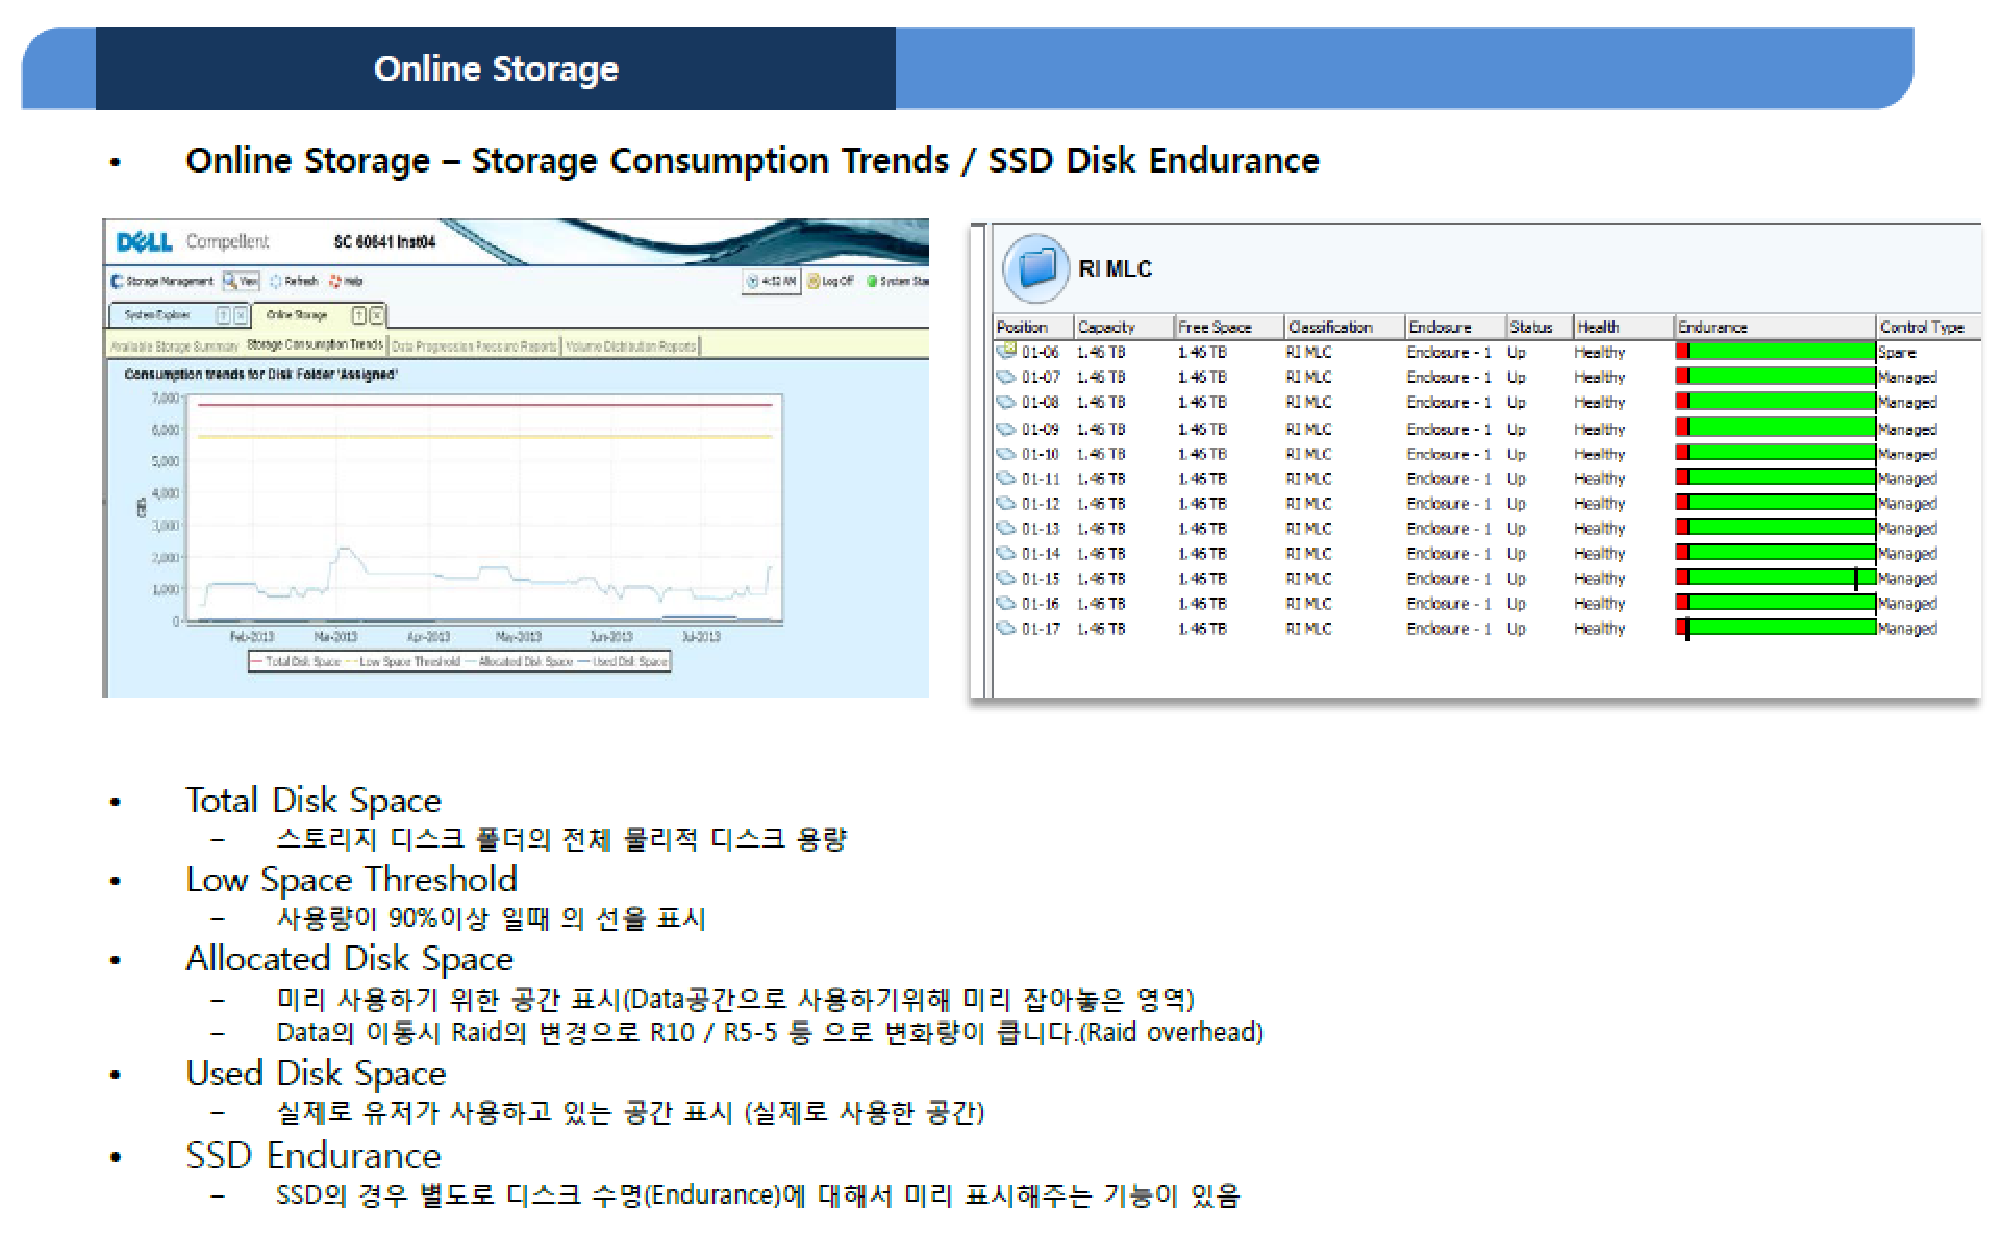
\includegraphics[width=0.85\textwidth]{./images/srfdb_storage_mana_12.eps}
	\caption{SRF Storage Management - 12}
	\label{fig:srfdb_mana_12} 
\end{figure}

\begin{figure}[h!]
	\centering
	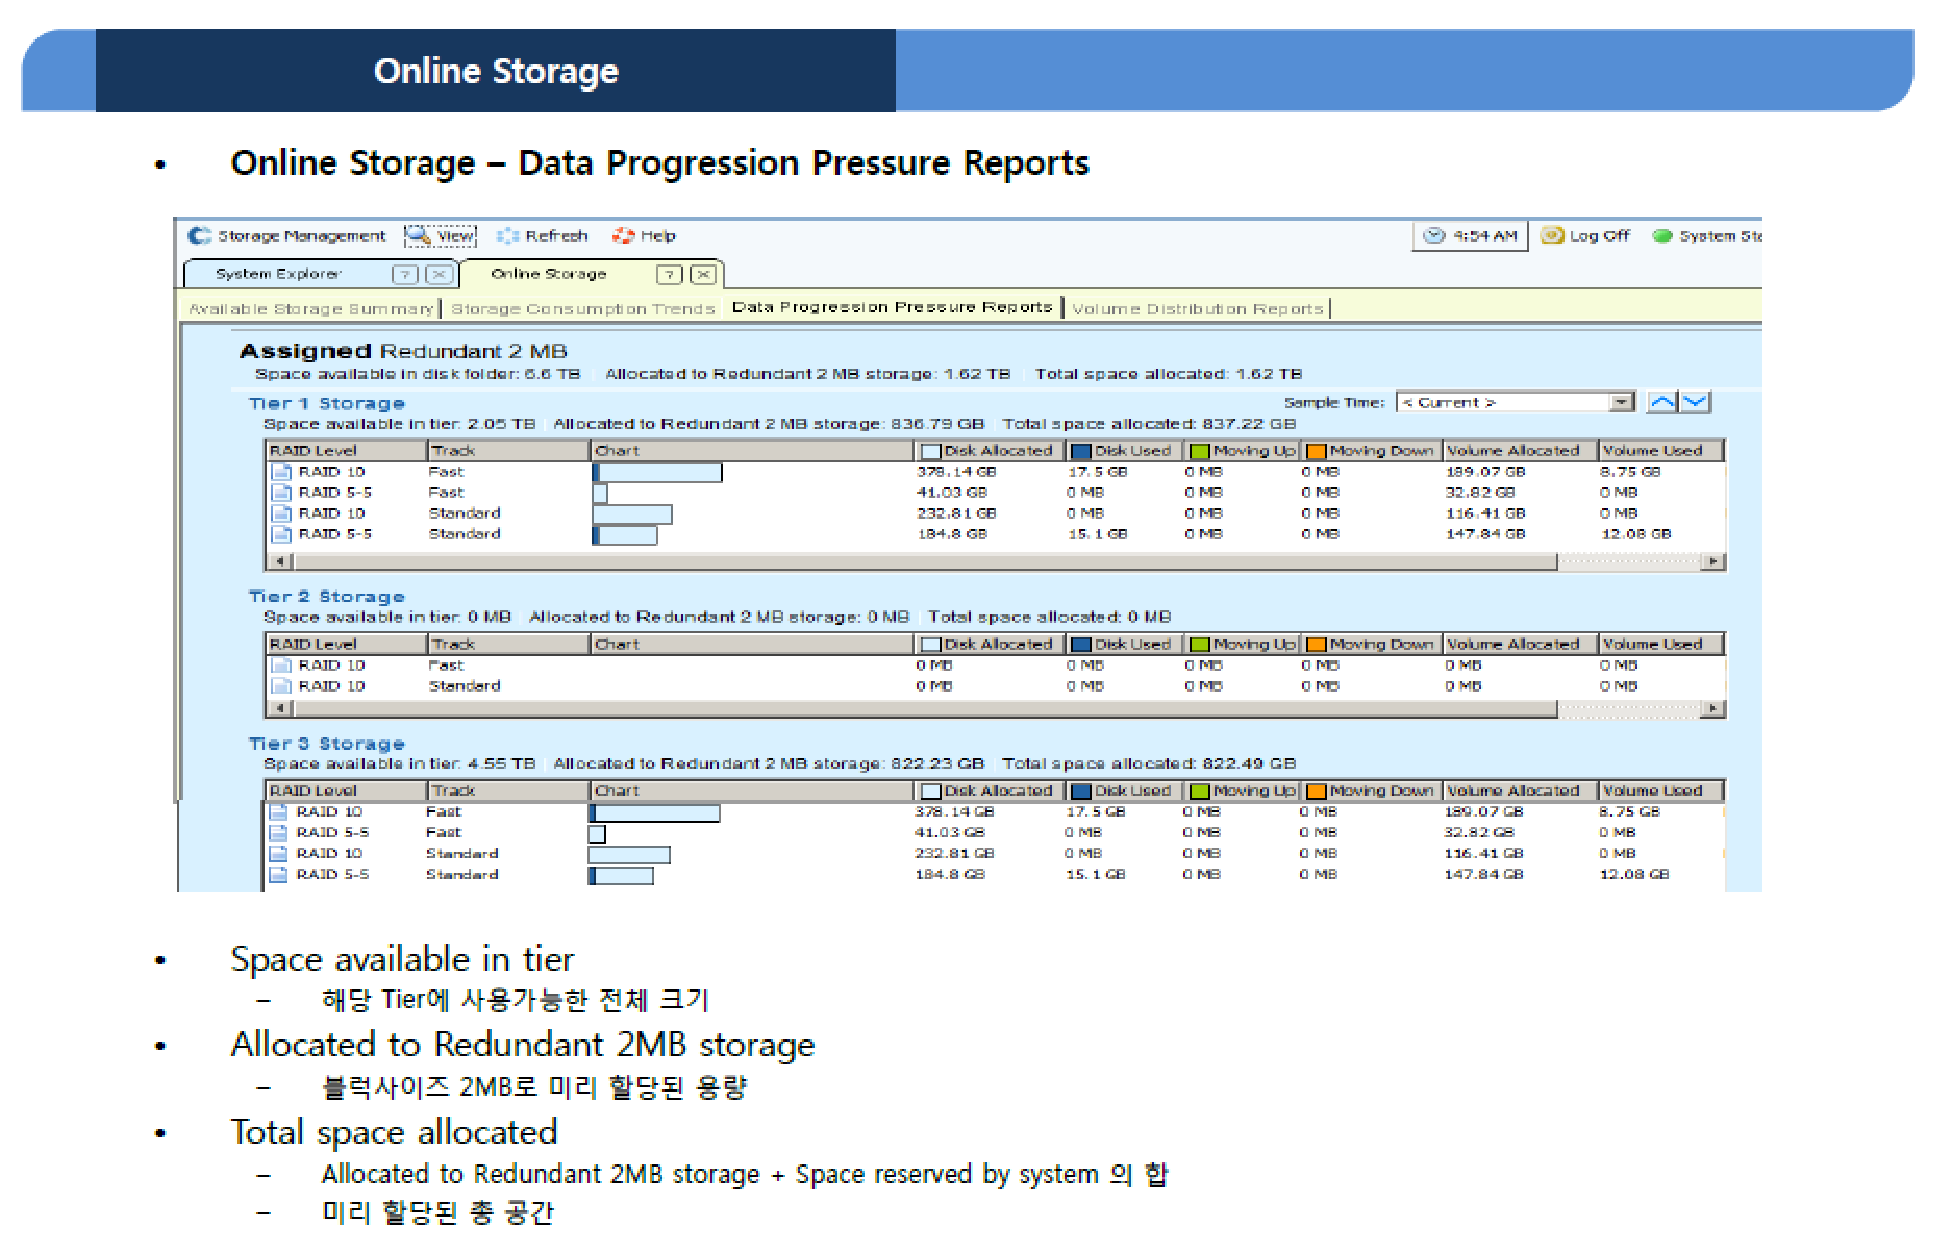
\includegraphics[width=0.85\textwidth]{./images/srfdb_storage_mana_13.eps}
	\caption{SRF Storage Management - 13}
	\label{fig:srfdb_mana_13} 
\end{figure}

\begin{figure}[h!]
	\centering
	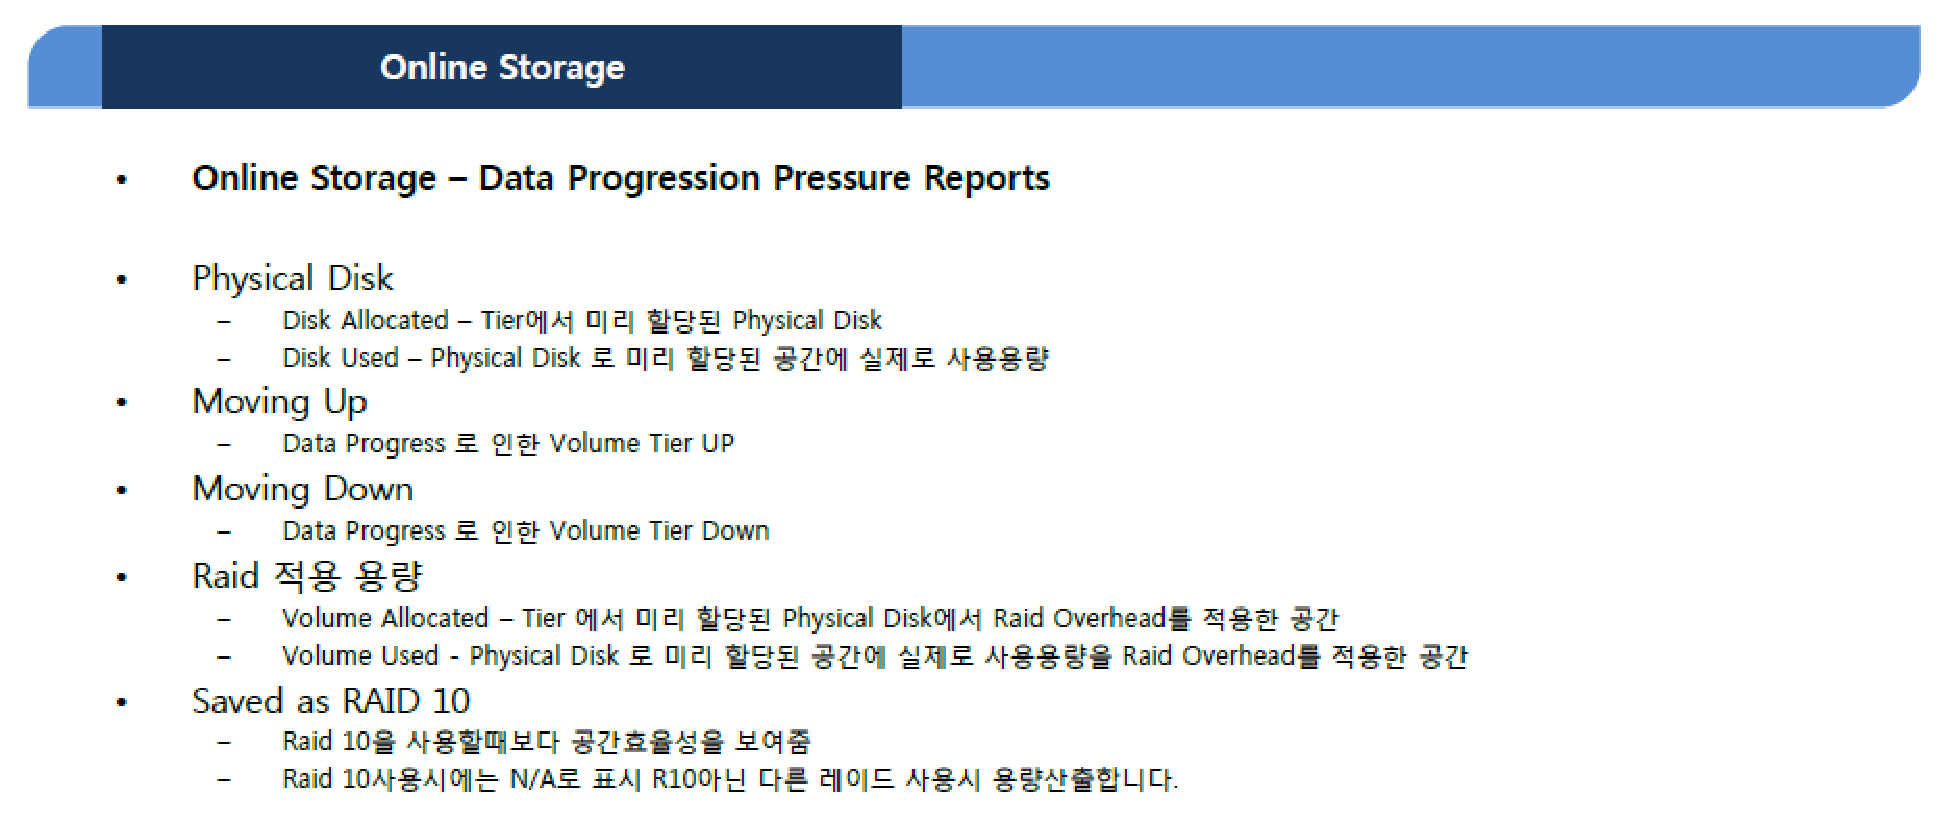
\includegraphics[width=0.85\textwidth]{./images/srfdb_storage_mana_14.eps}
	\caption{SRF Storage Management - 14}
	\label{fig:srfdb_mana_14} 
\end{figure}

\begin{figure}[h!]
	\centering
	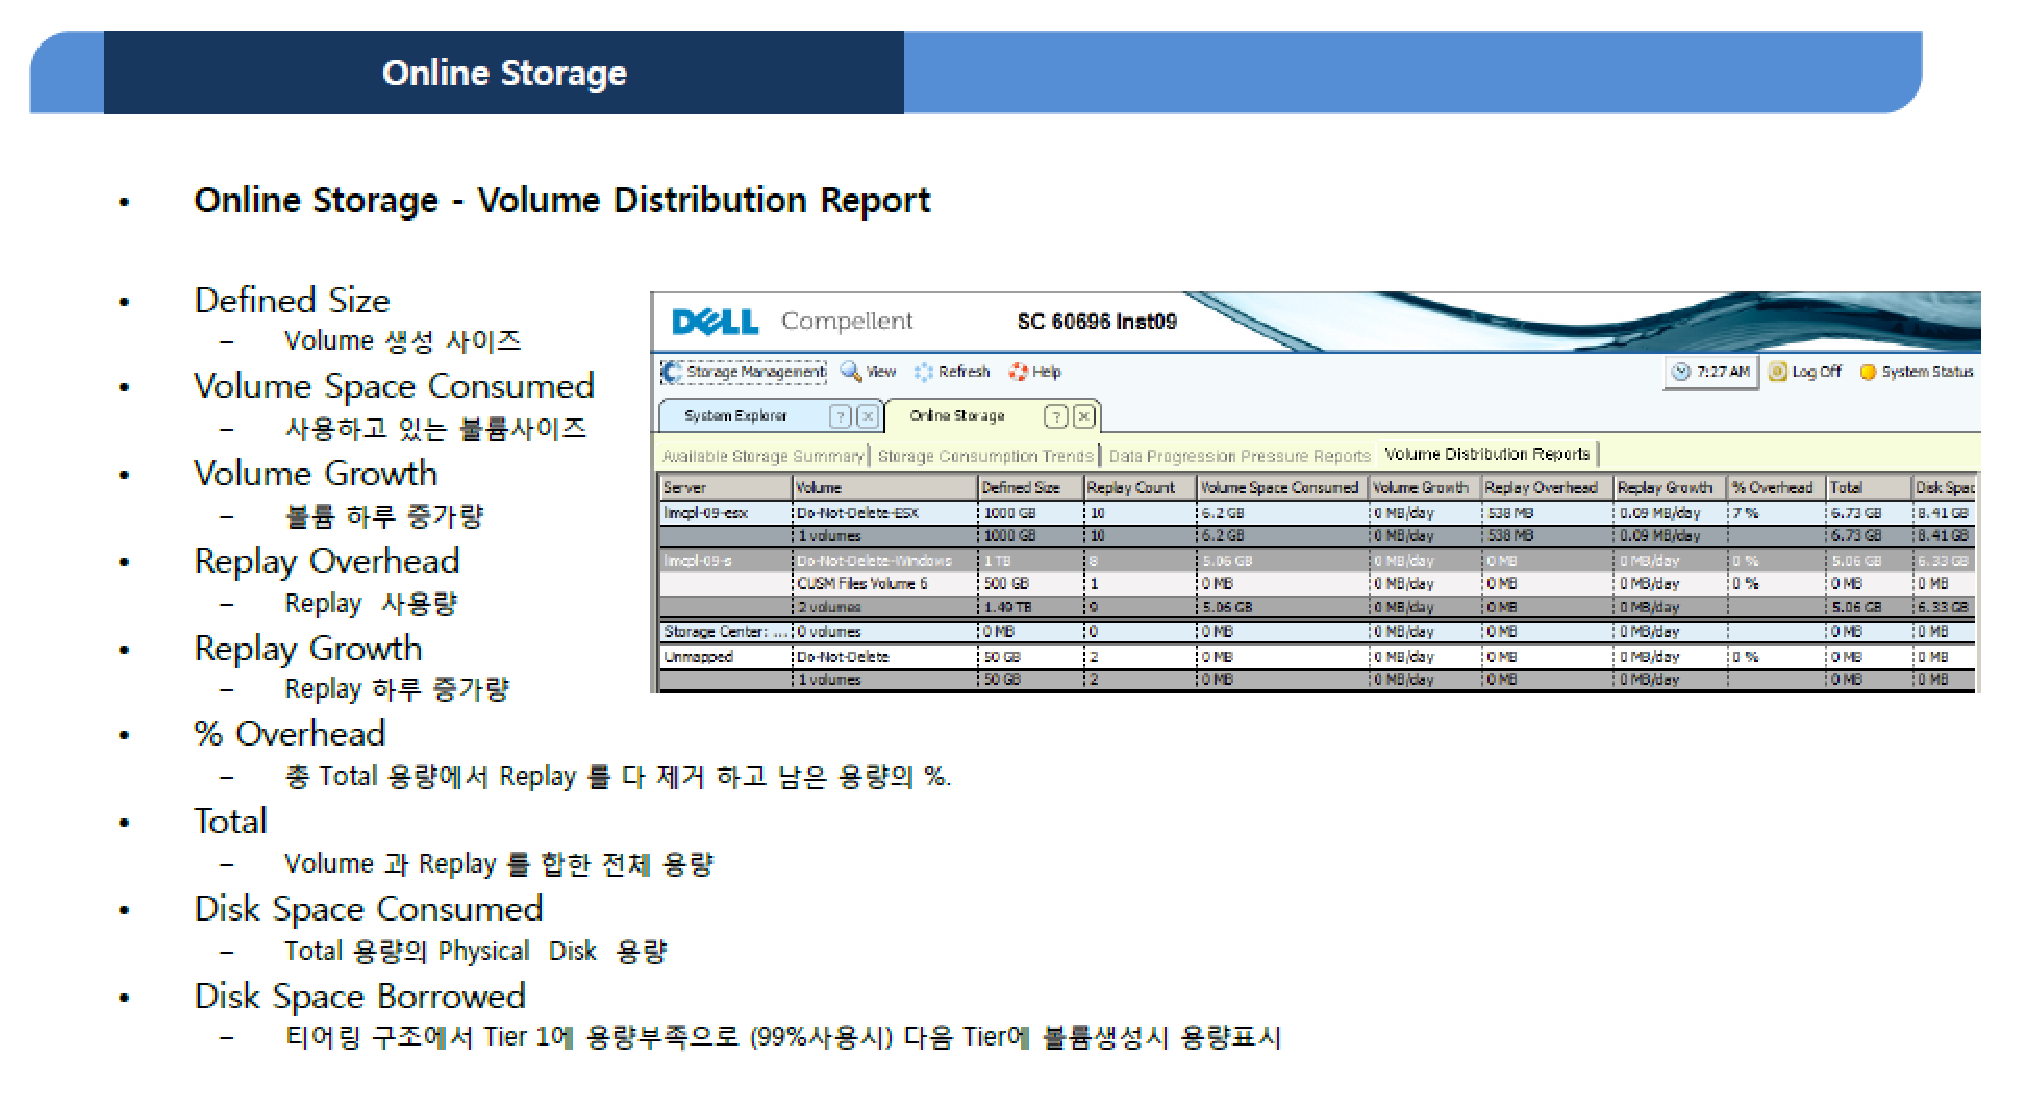
\includegraphics[width=0.85\textwidth]{./images/srfdb_storage_mana_15.eps}
	\caption{SRF Storage Management - 15}
	\label{fig:srfdb_mana_15} 
\end{figure}

\begin{figure}[h!]
	\centering
	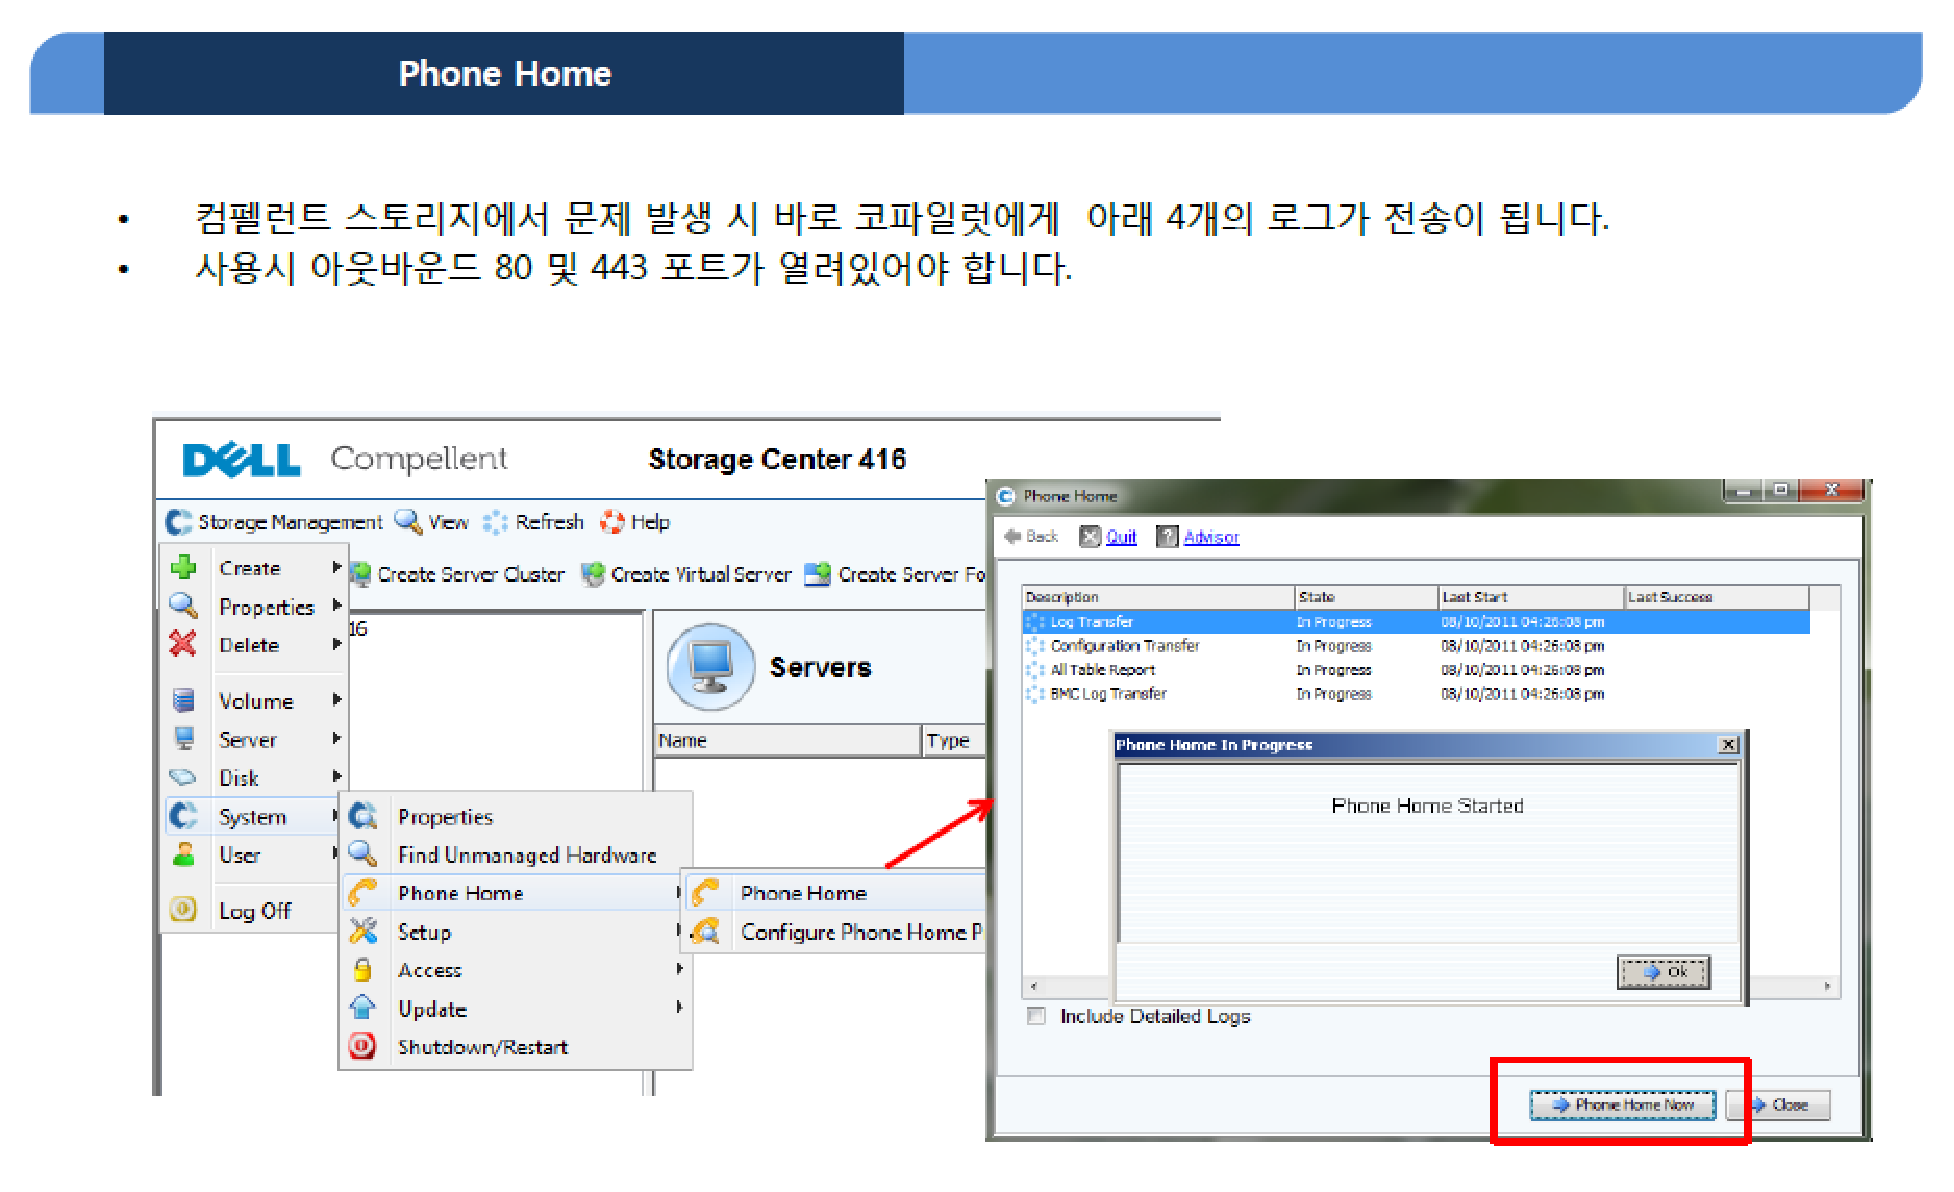
\includegraphics[width=0.85\textwidth]{./images/srfdb_storage_mana_16.eps}
	\caption{SRF Storage Management - 16}
	\label{fig:srfdb_mana_16} 
\end{figure}

\begin{figure}[h!]
	\centering
	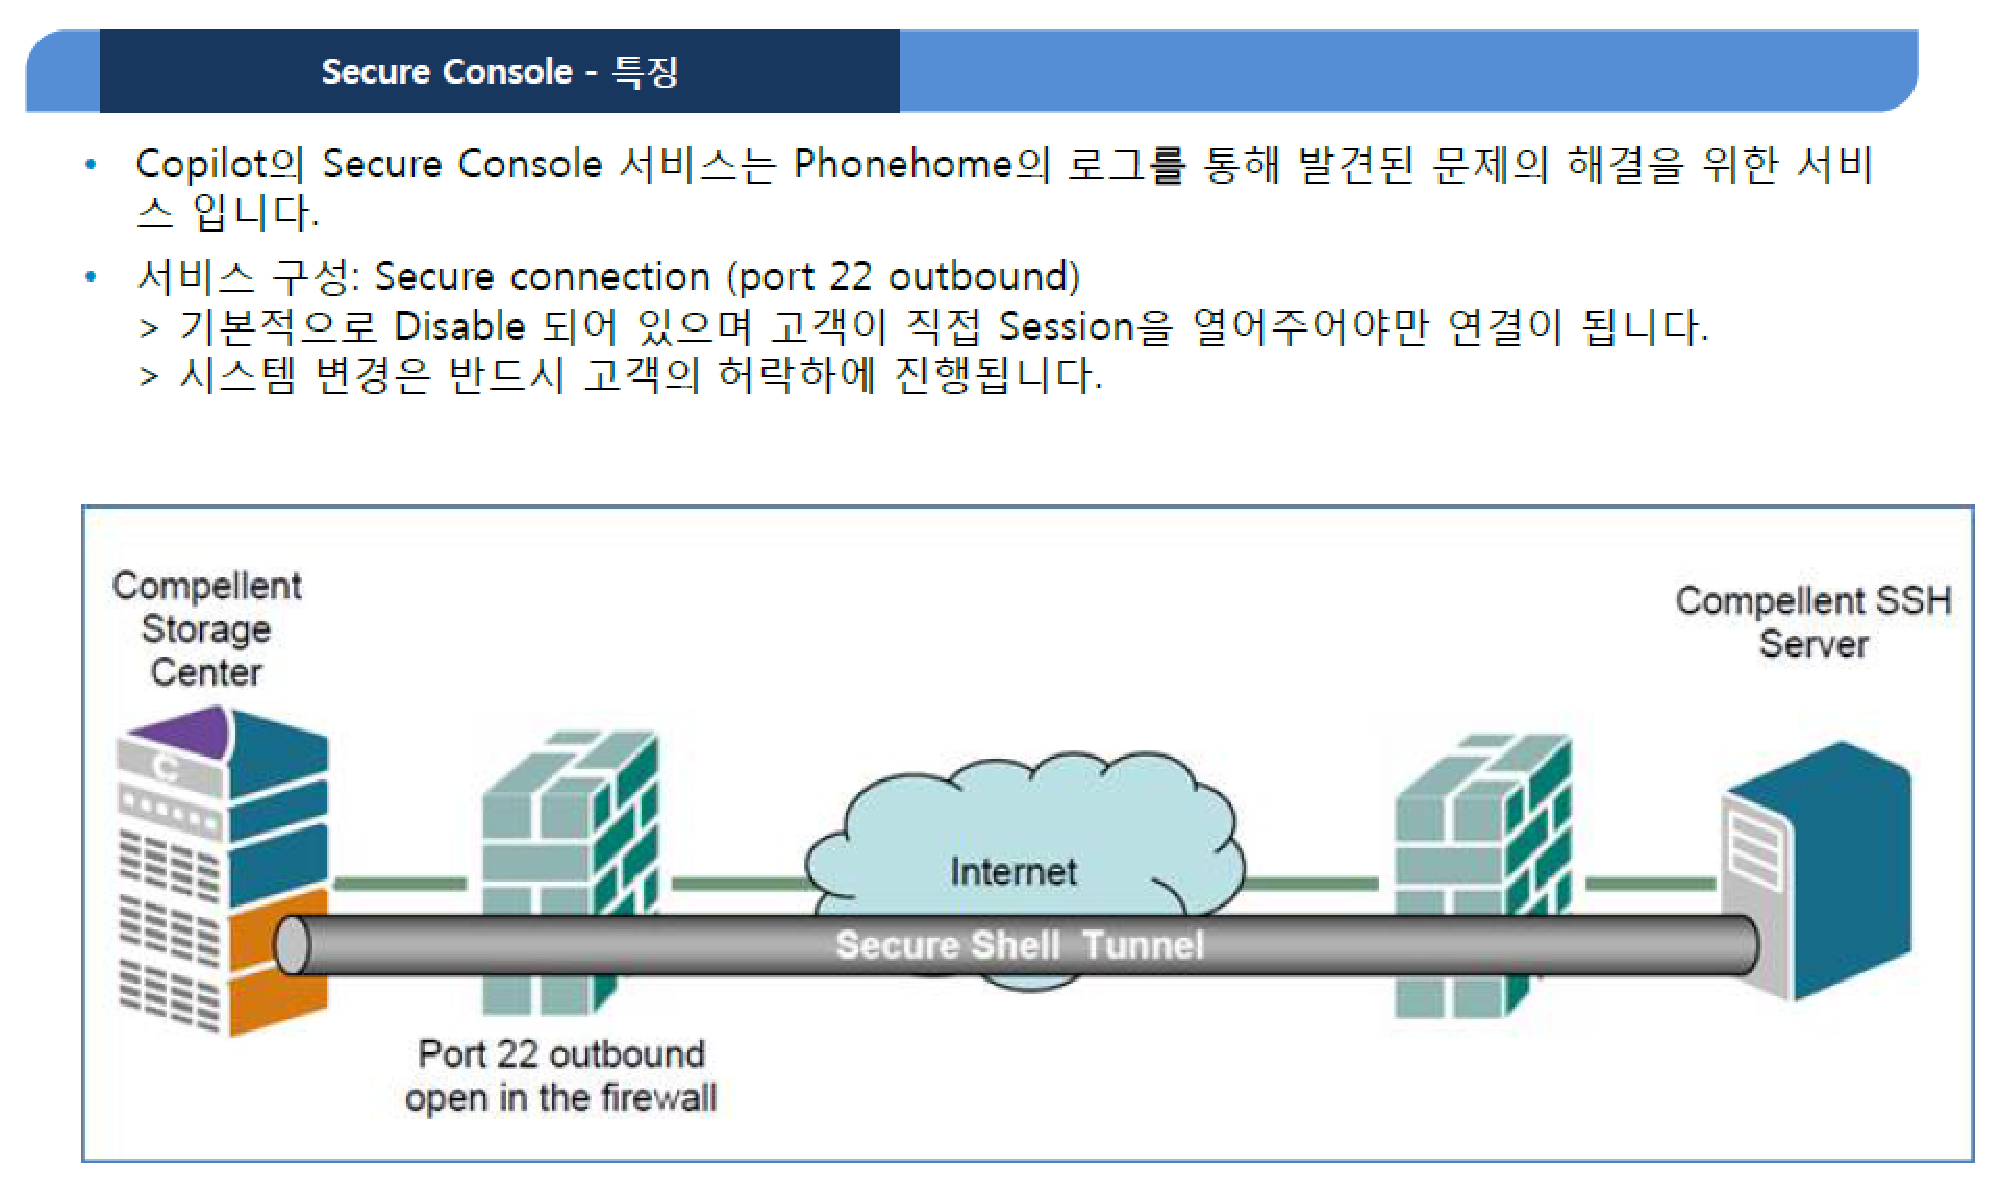
\includegraphics[width=0.85\textwidth]{./images/srfdb_storage_mana_17.eps}
	\caption{SRF Storage Management - 17}
	\label{fig:srfdb_mana_17} 
\end{figure}

\begin{figure}[h!]
	\centering
	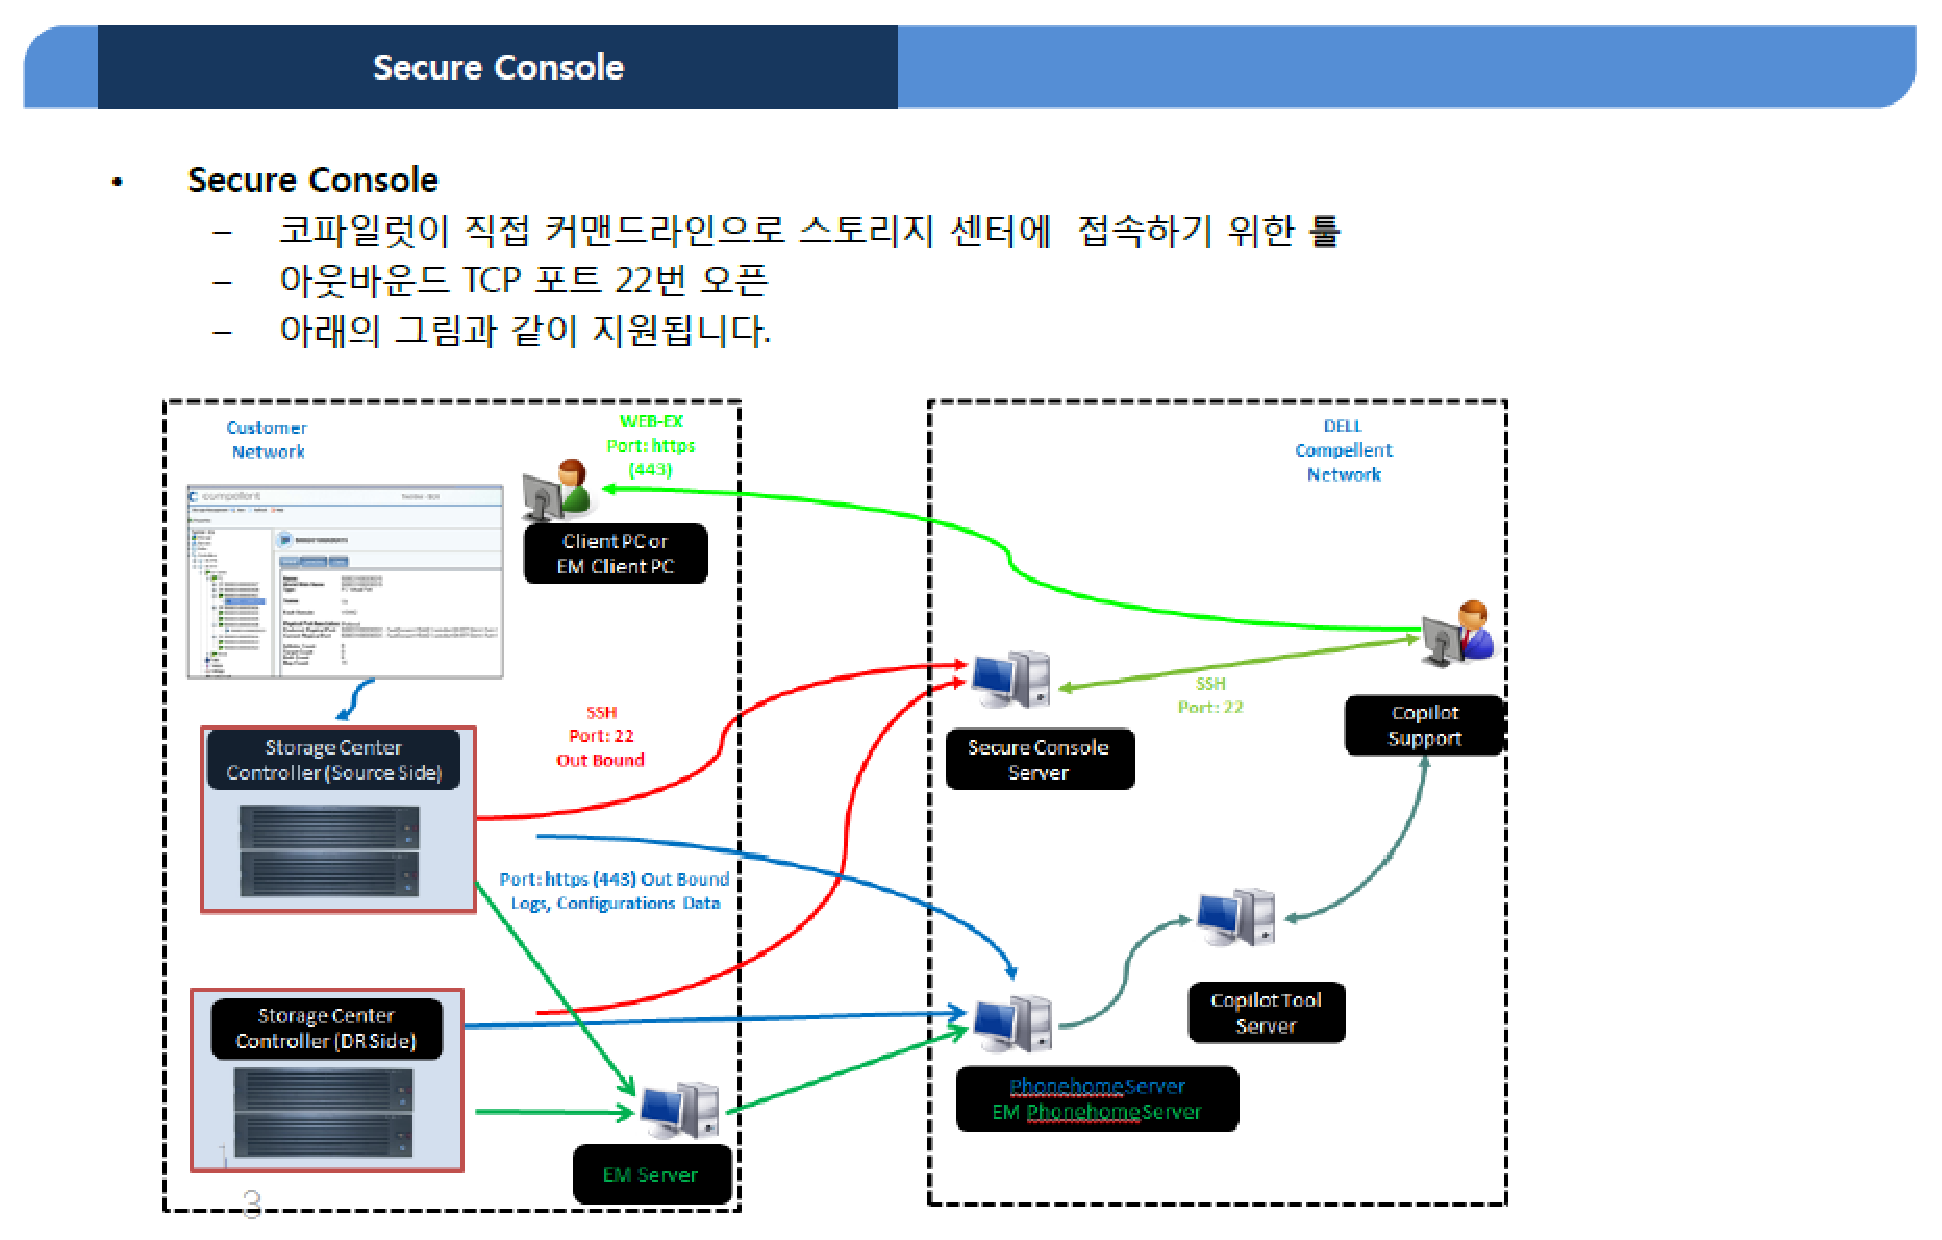
\includegraphics[width=0.85\textwidth]{./images/srfdb_storage_mana_18.eps}
	\caption{SRF Storage Management - 18}
	\label{fig:srfdb_mana_18} 
\end{figure}

\clearpage

\begin{figure}[h!]
	\centering
	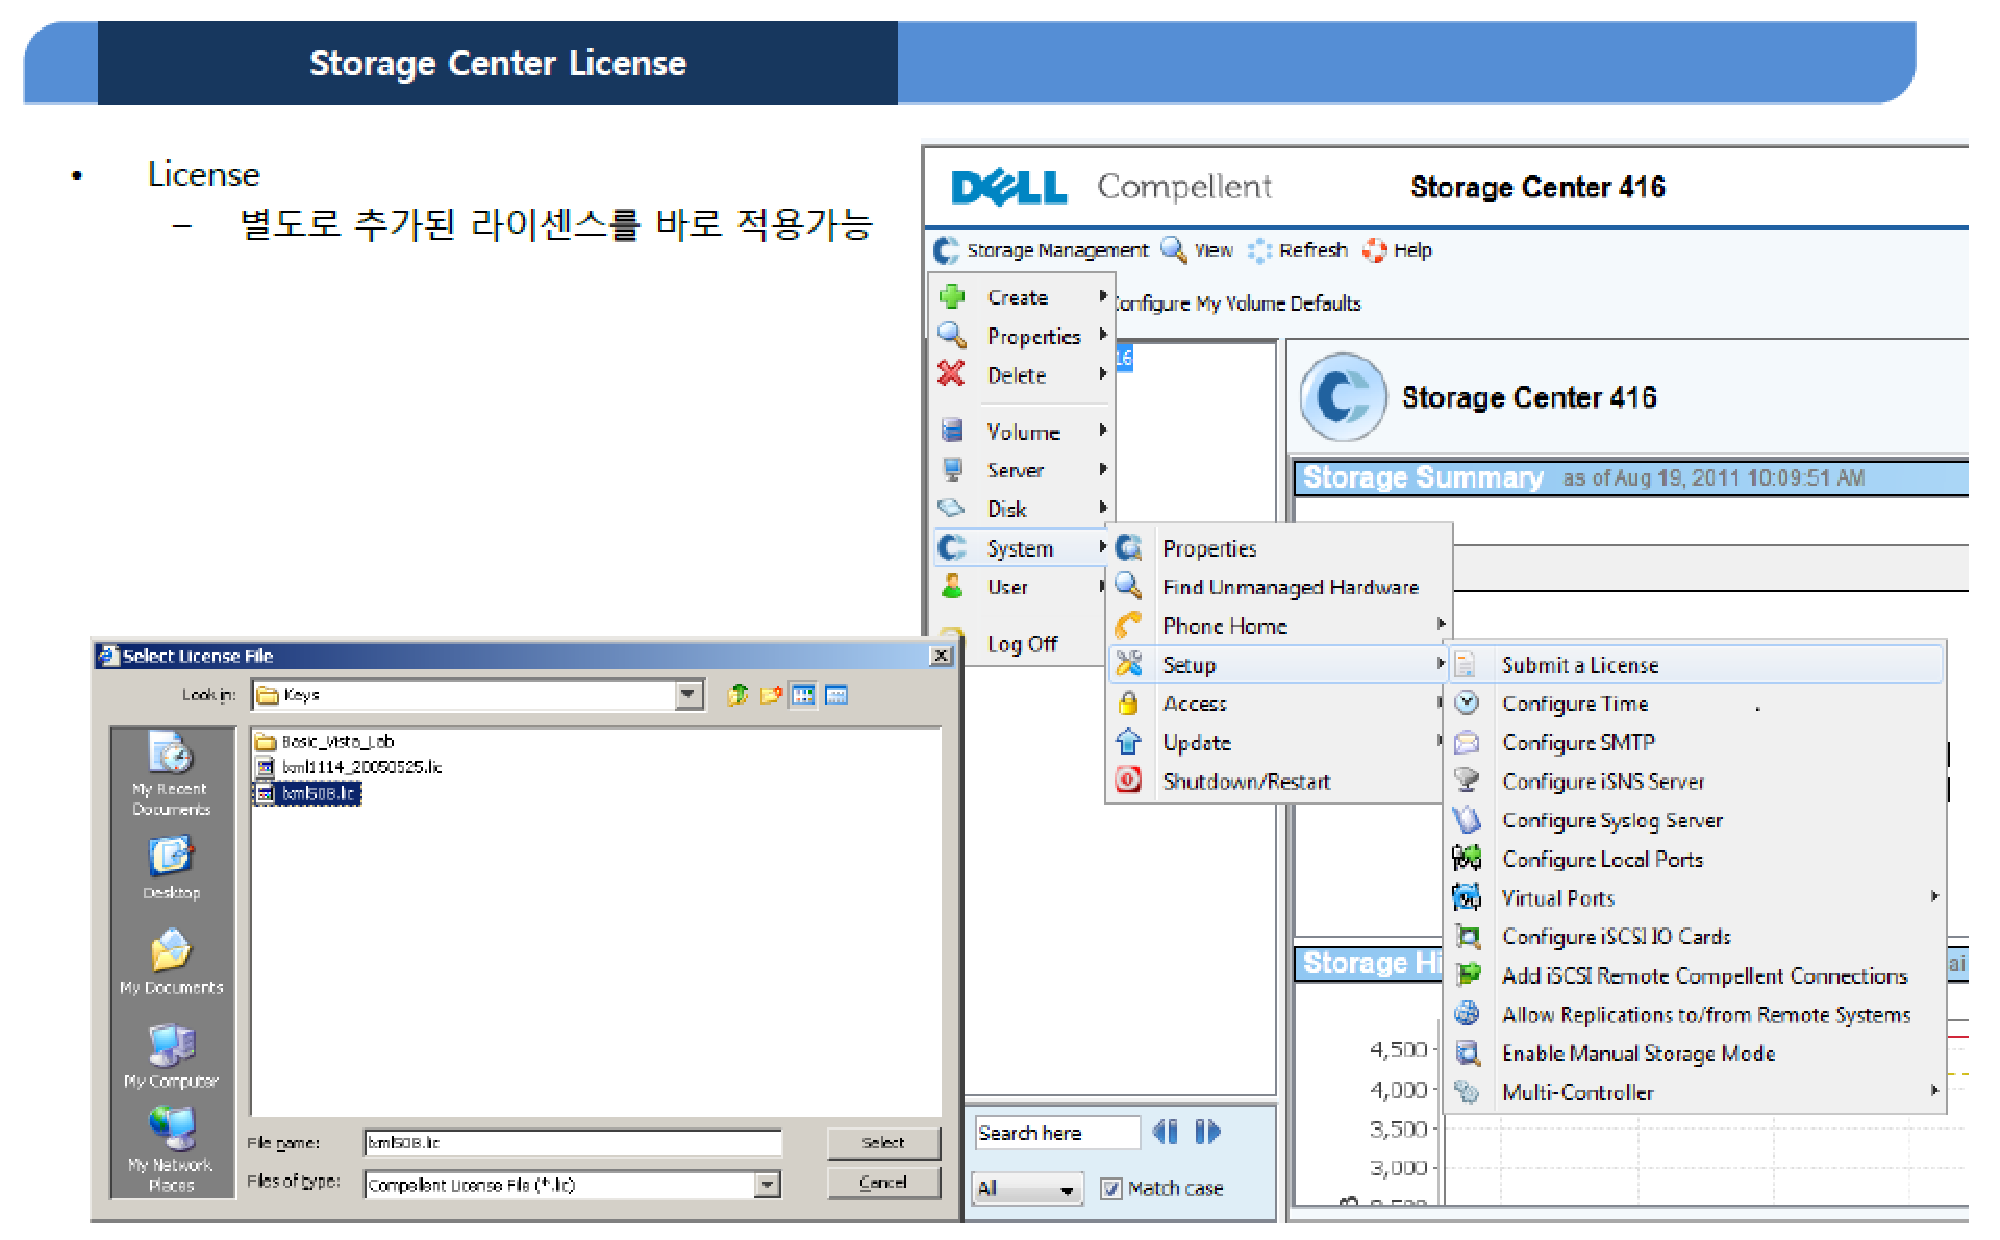
\includegraphics[width=0.85\textwidth]{./images/srfdb_storage_mana_19.eps}
	\caption{SRF Storage Management - 19}
	\label{fig:srfdb_mana_19} 
\end{figure}

\begin{figure}[h!]
	\centering
	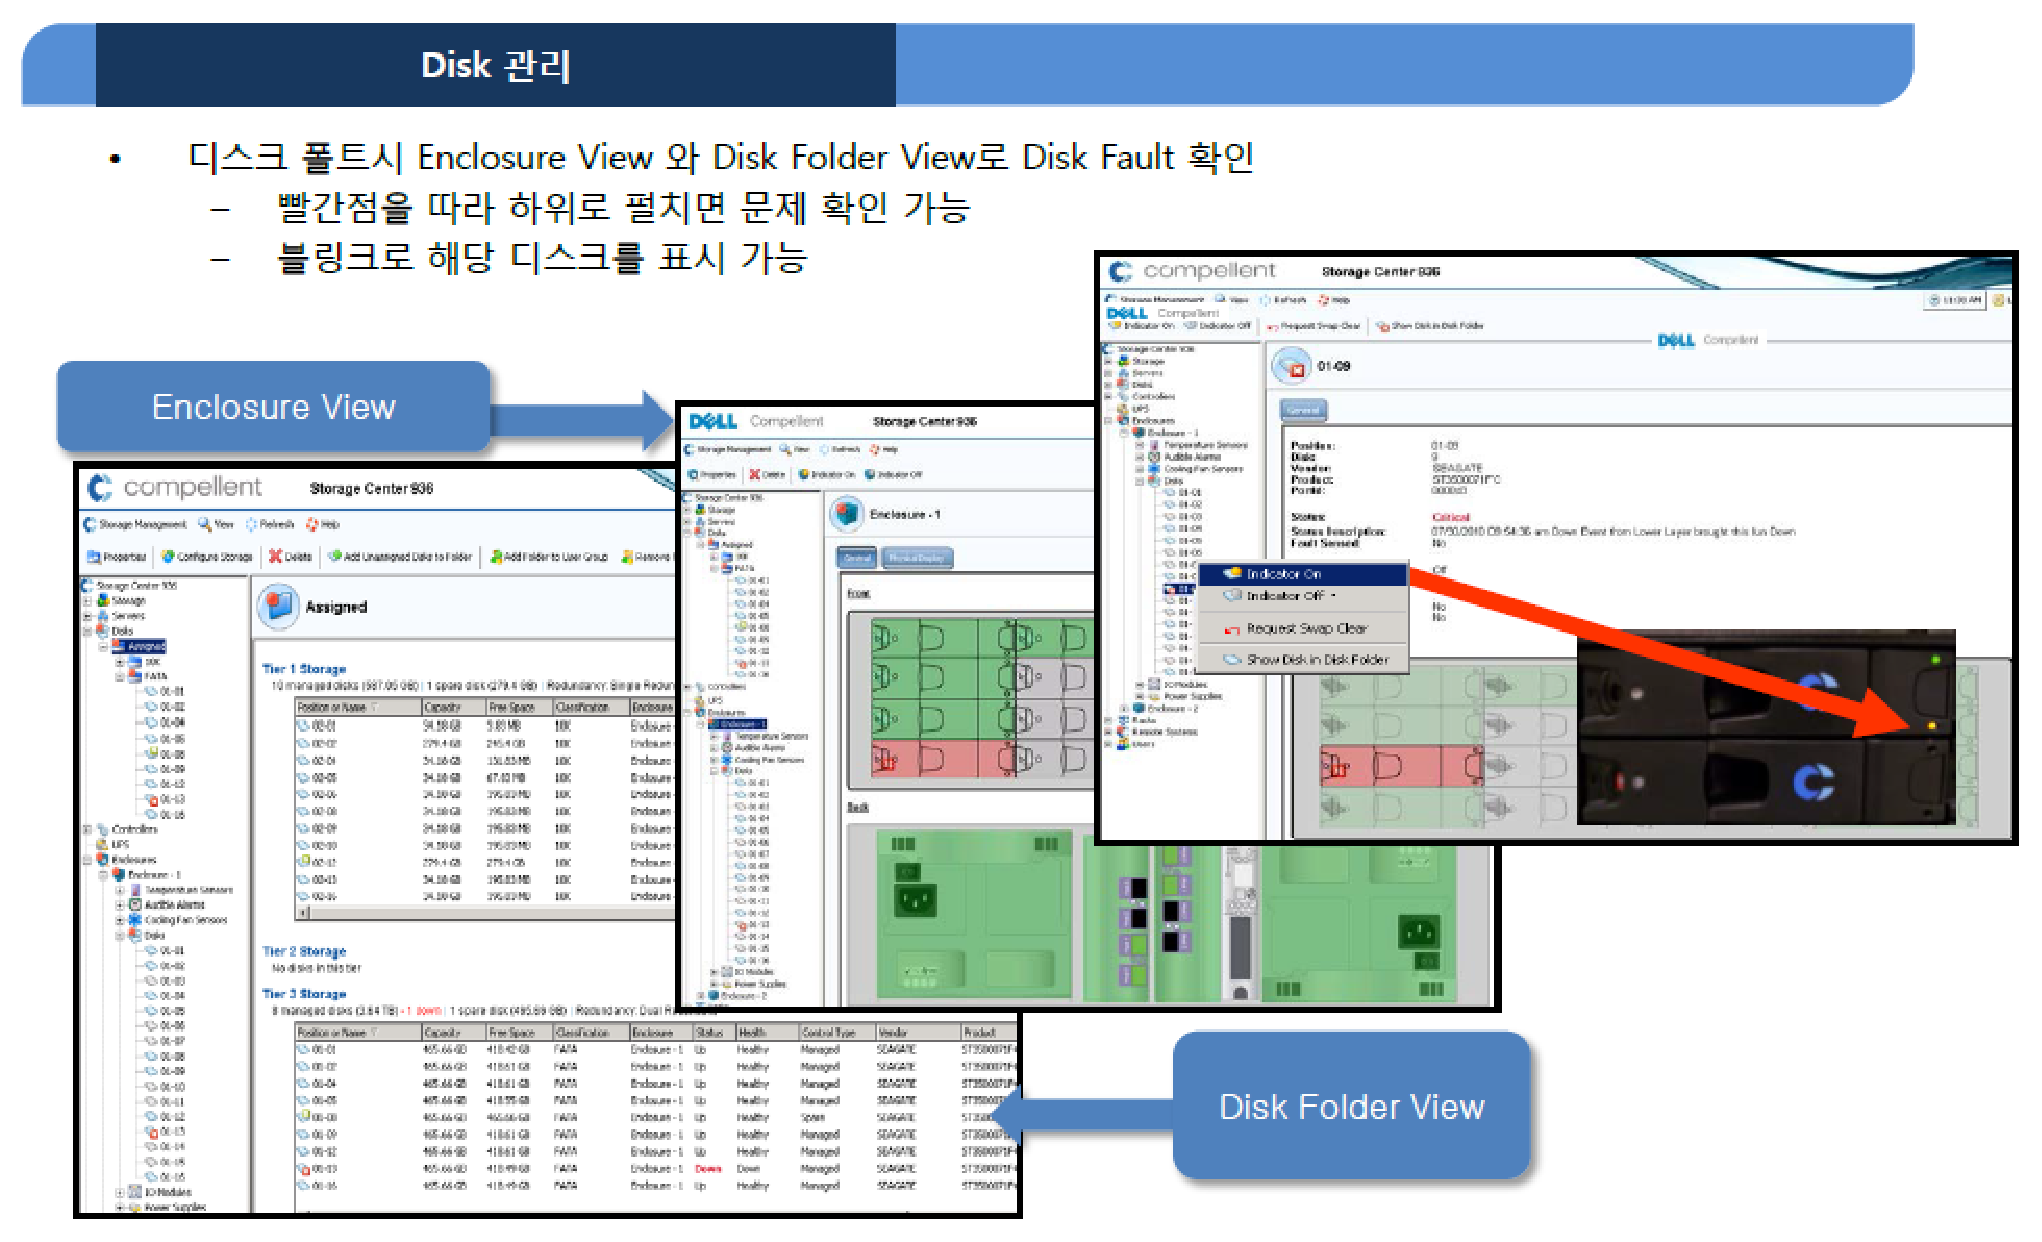
\includegraphics[width=0.85\textwidth]{./images/srfdb_storage_mana_20.eps}
	\caption{SRF Storage Management - 20}
	\label{fig:srfdb_mana_20} 
\end{figure}

\begin{figure}[h!]
	\centering
	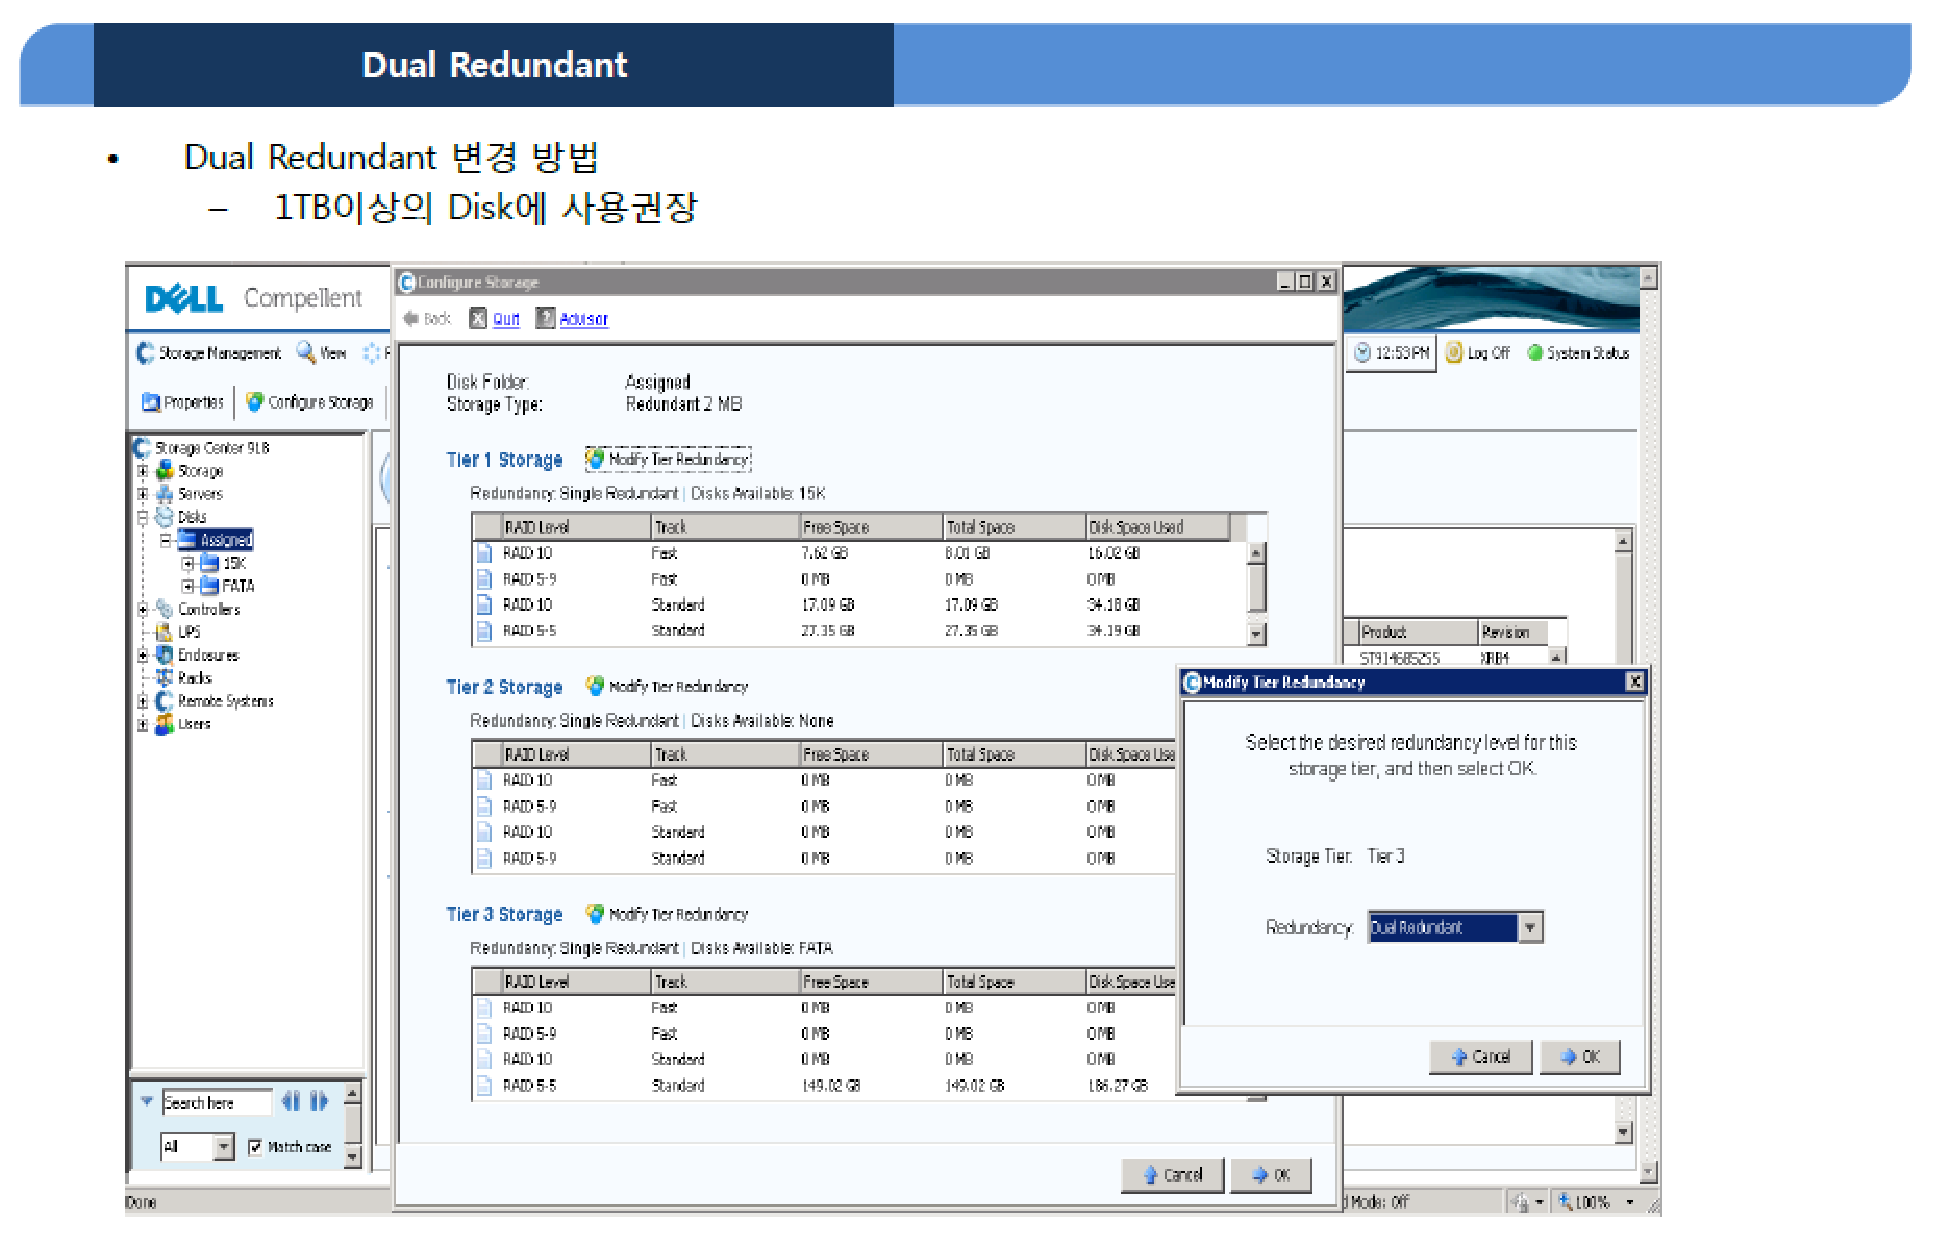
\includegraphics[width=0.85\textwidth]{./images/srfdb_storage_mana_21.eps}
	\caption{SRF Storage Management - 21}
	\label{fig:srfdb_mana_21} 
\end{figure}

\begin{figure}[h!]
	\centering
	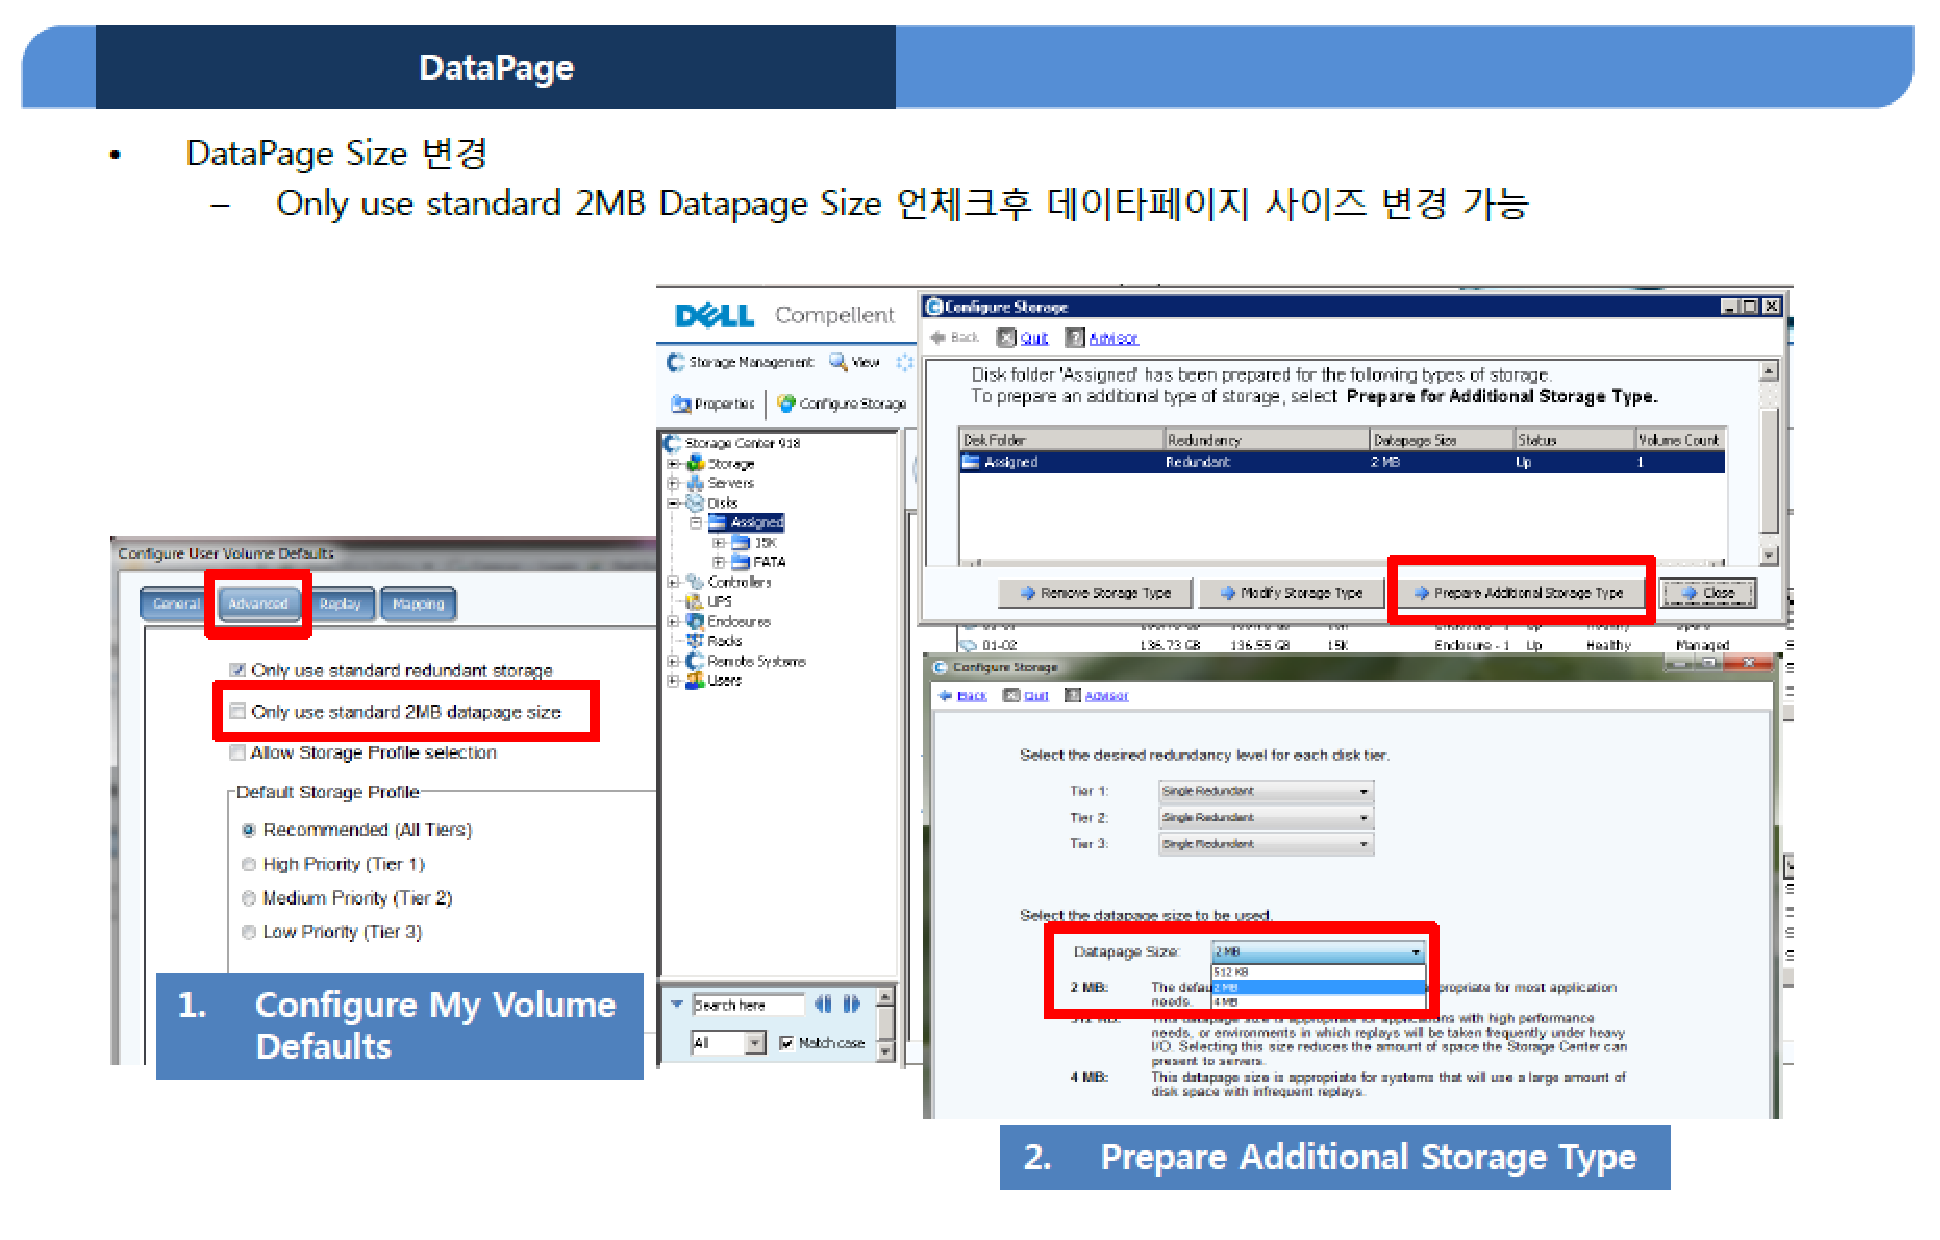
\includegraphics[width=0.85\textwidth]{./images/srfdb_storage_mana_22.eps}
	\caption{SRF Storage Management - 22}
	\label{fig:srfdb_mana_22} 
\end{figure}

\begin{figure}[h!]
	\centering
	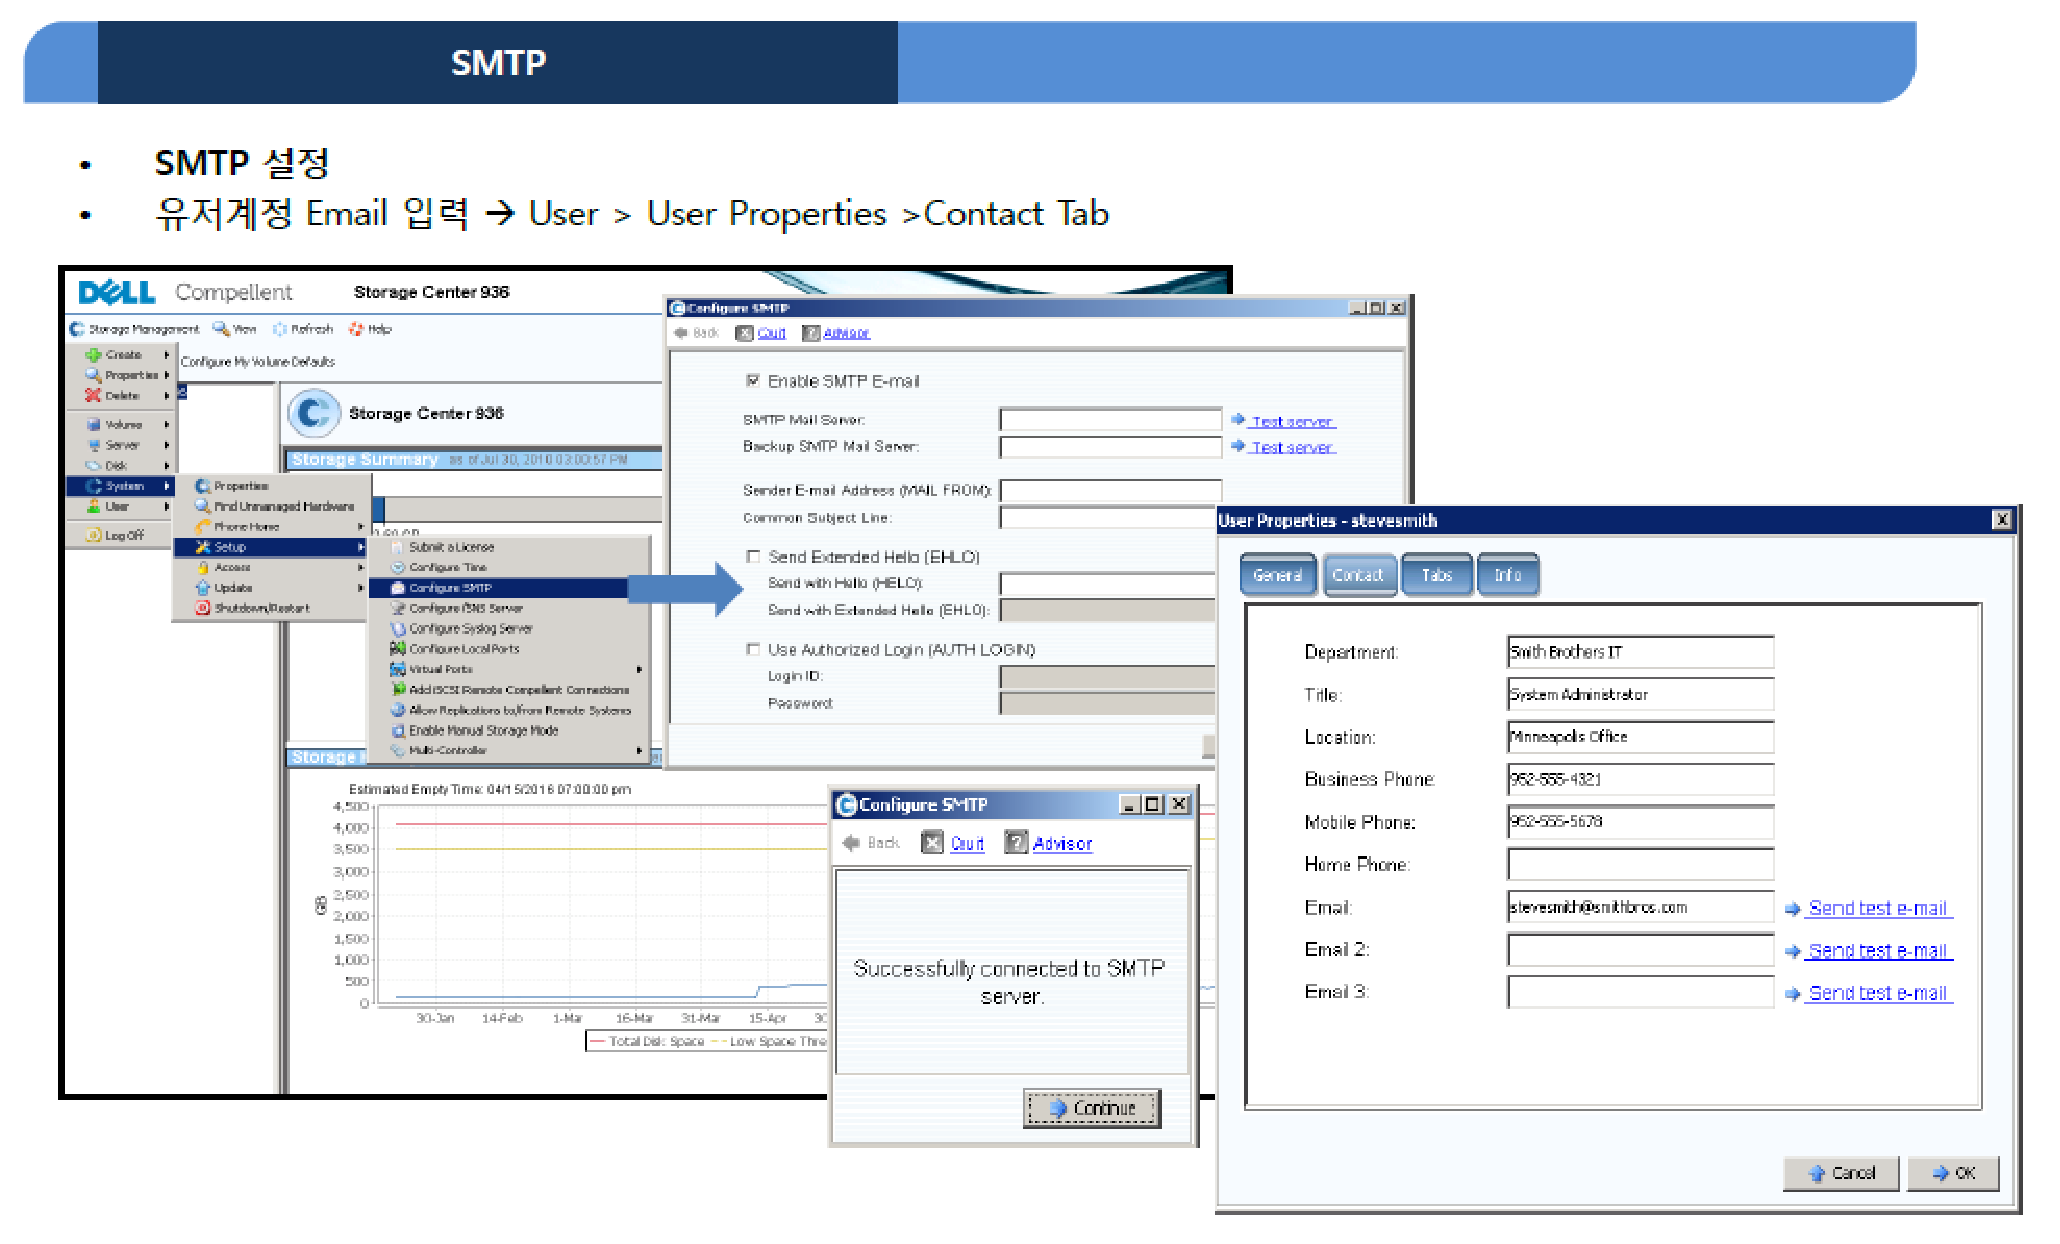
\includegraphics[width=0.85\textwidth]{./images/srfdb_storage_mana_23.eps}
	\caption{SRF Storage Management - 23}
	\label{fig:srfdb_mana_23} 
\end{figure}

\begin{figure}[h!]
	\centering
	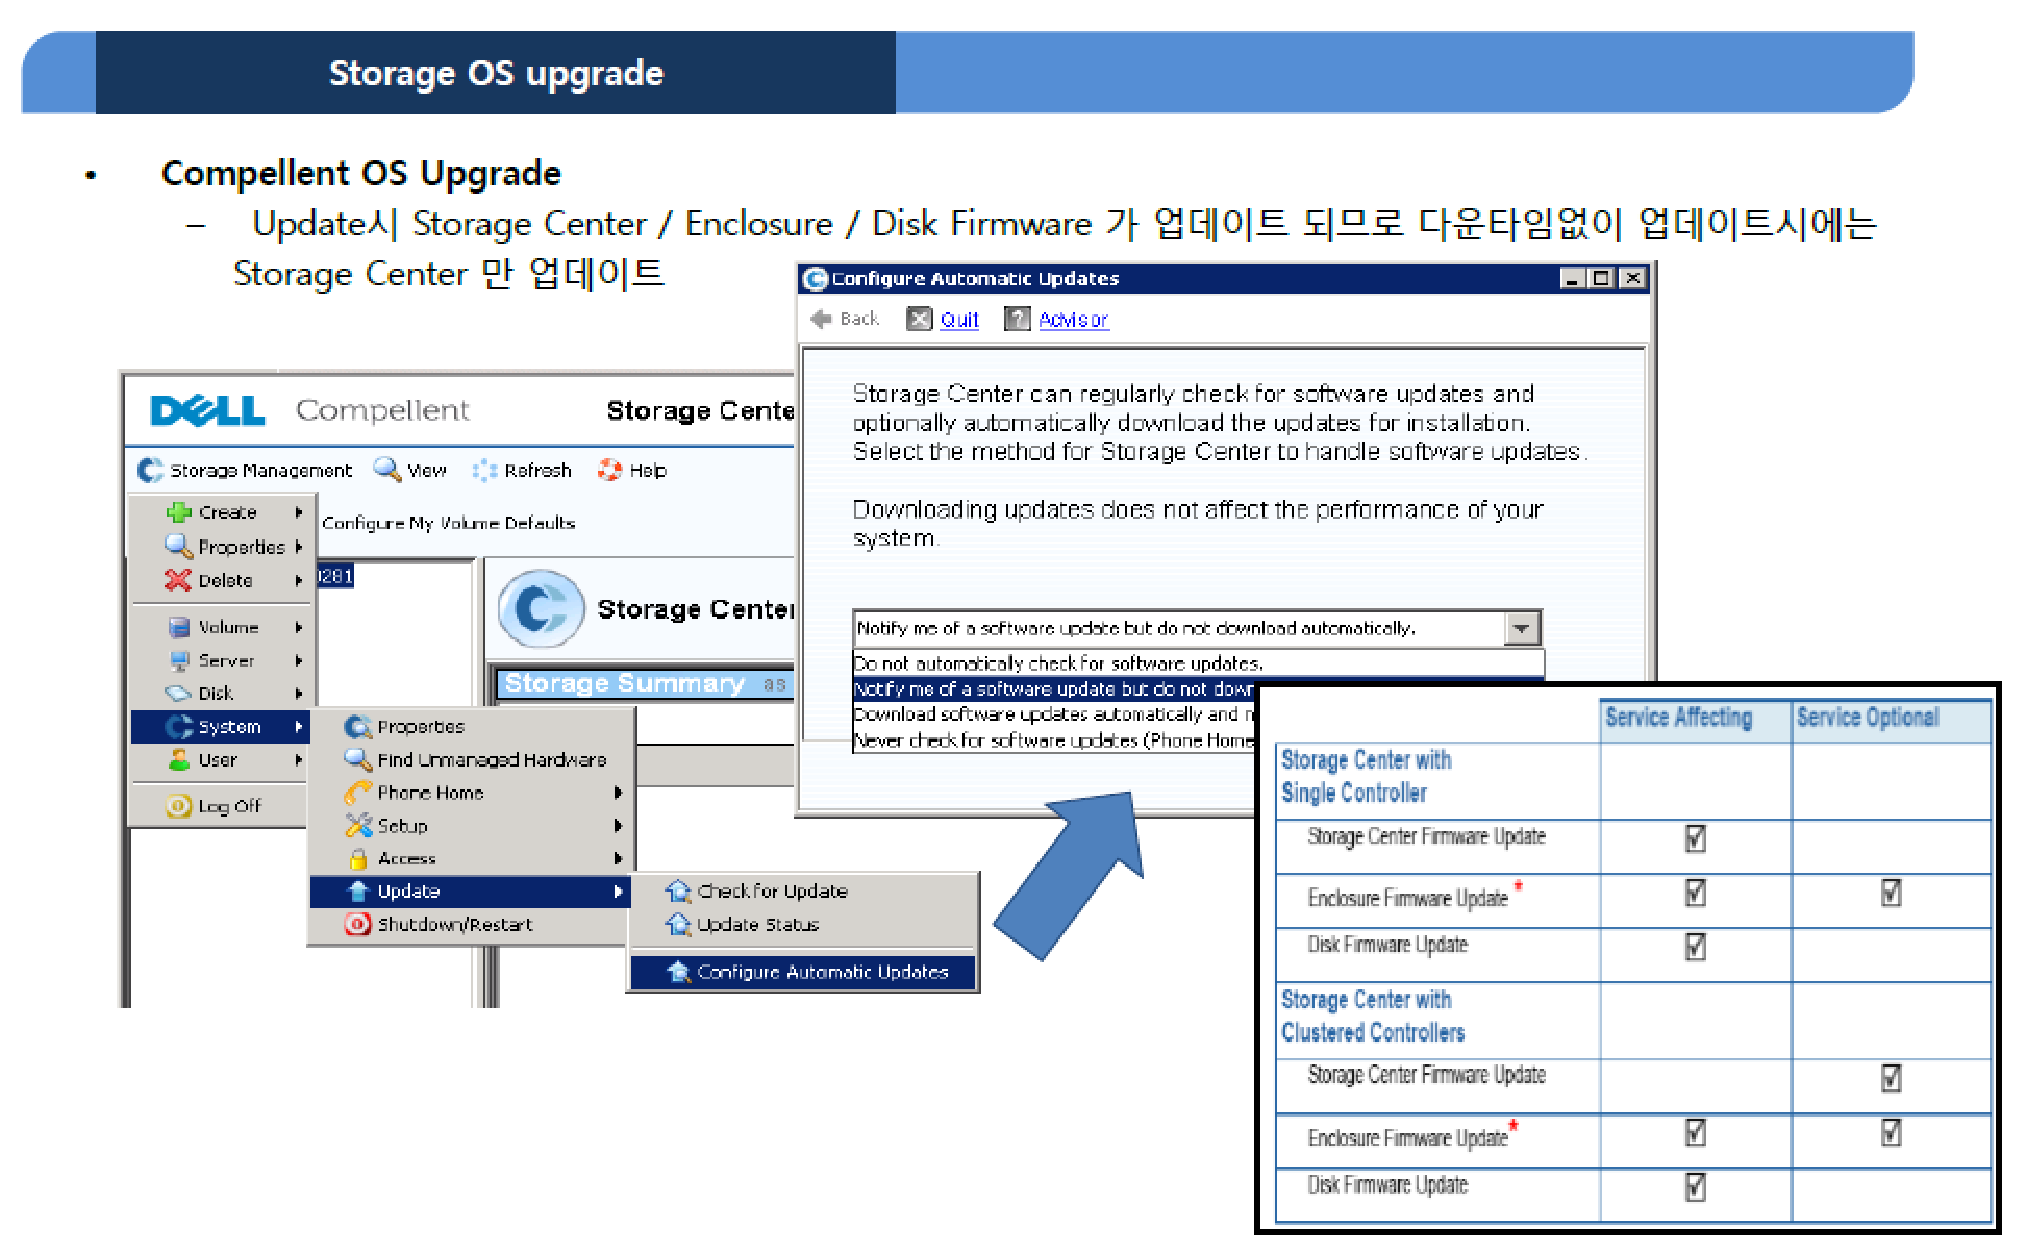
\includegraphics[width=0.85\textwidth]{./images/srfdb_storage_mana_24.eps}
	\caption{SRF Storage Management - 24}
	\label{fig:srfdb_mana_24} 
\end{figure}

\begin{figure}[h!]
	\centering
	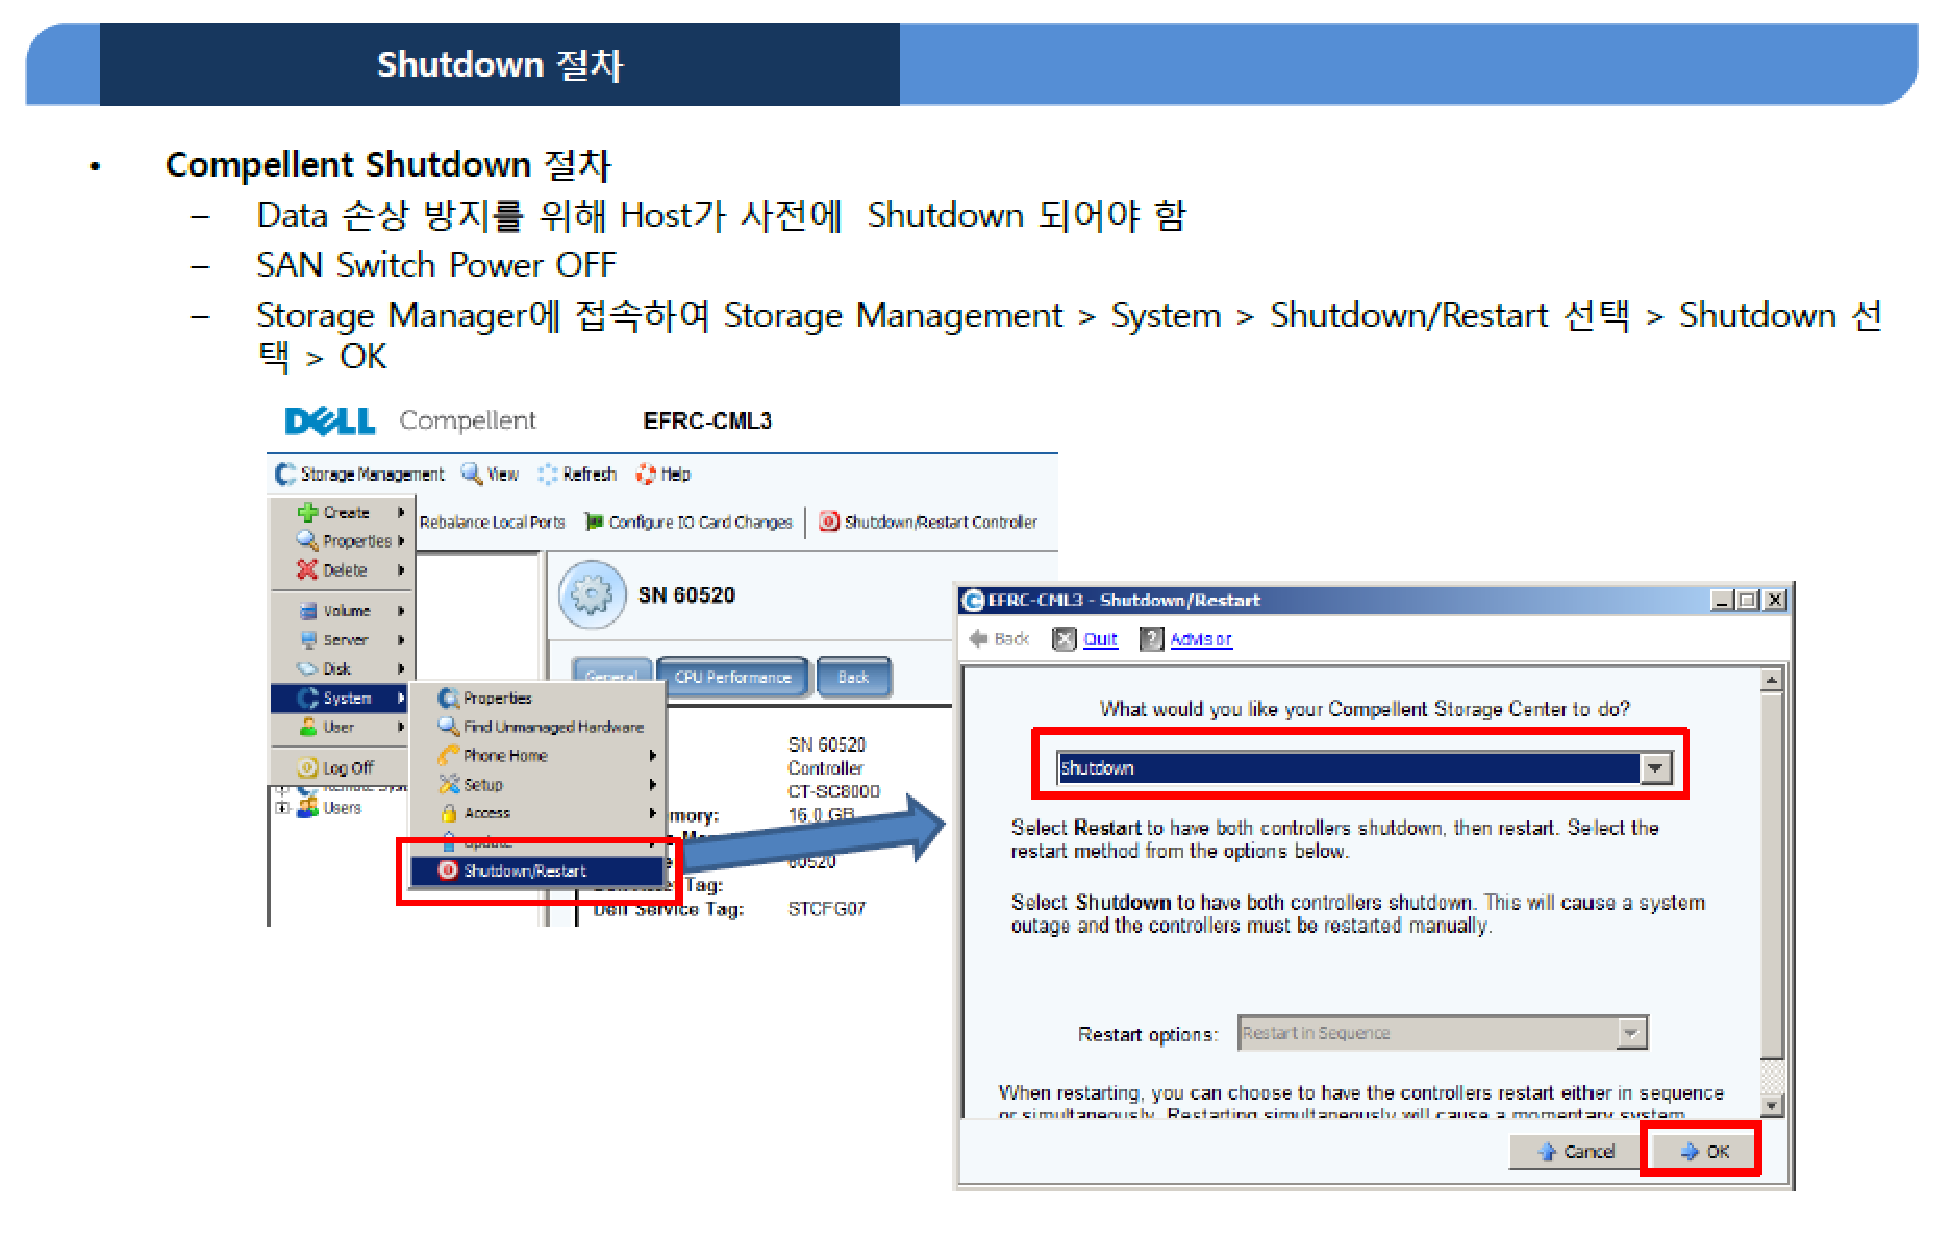
\includegraphics[width=0.85\textwidth]{./images/srfdb_storage_mana_25.eps}
	\caption{SRF Storage Management - 25}
	\label{fig:srfdb_mana_25} 
\end{figure}

\begin{figure}[h!]
	\centering
	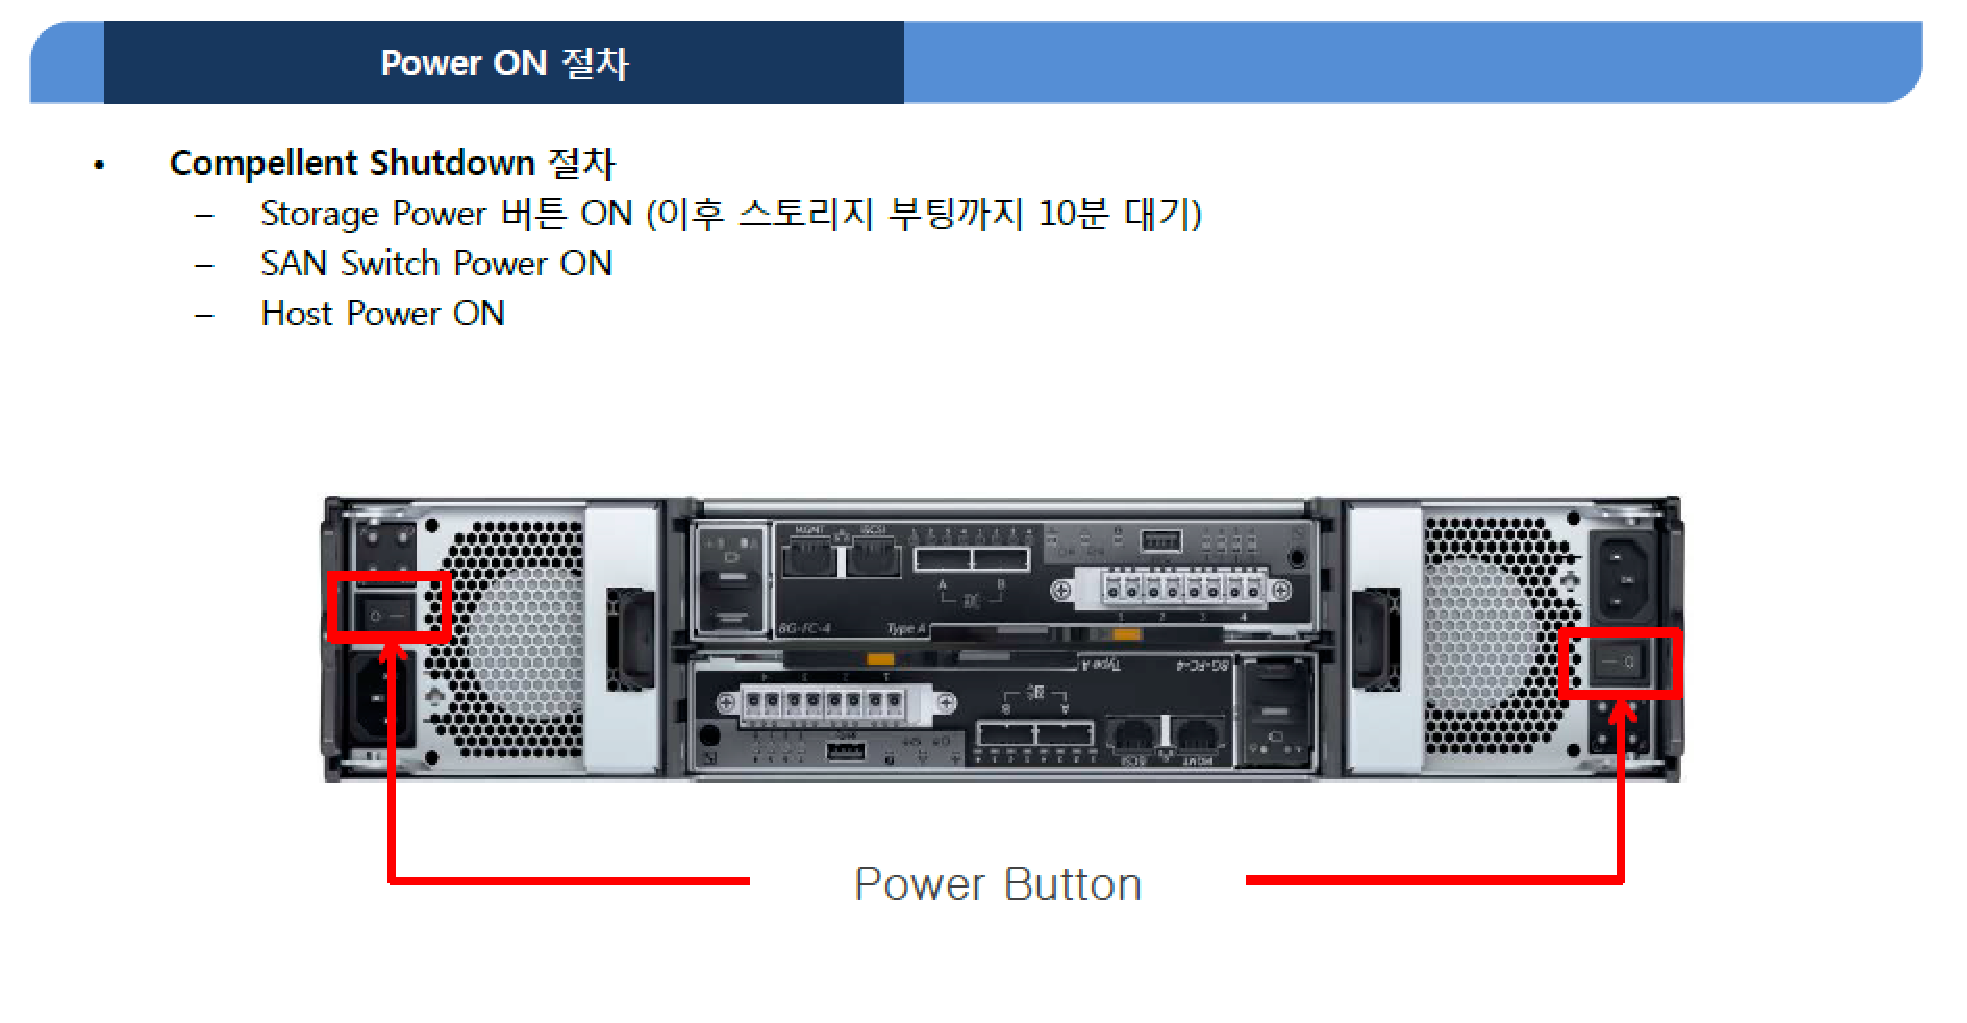
\includegraphics[width=0.85\textwidth]{./images/srfdb_storage_mana_26.eps}
	\caption{SRF Storage Management - 26}
	\label{fig:srfdb_mana_26} 
\end{figure}

\clearpage
\section{성능 시험}

\clearpage

\begin{figure}[h!]
	\centering
	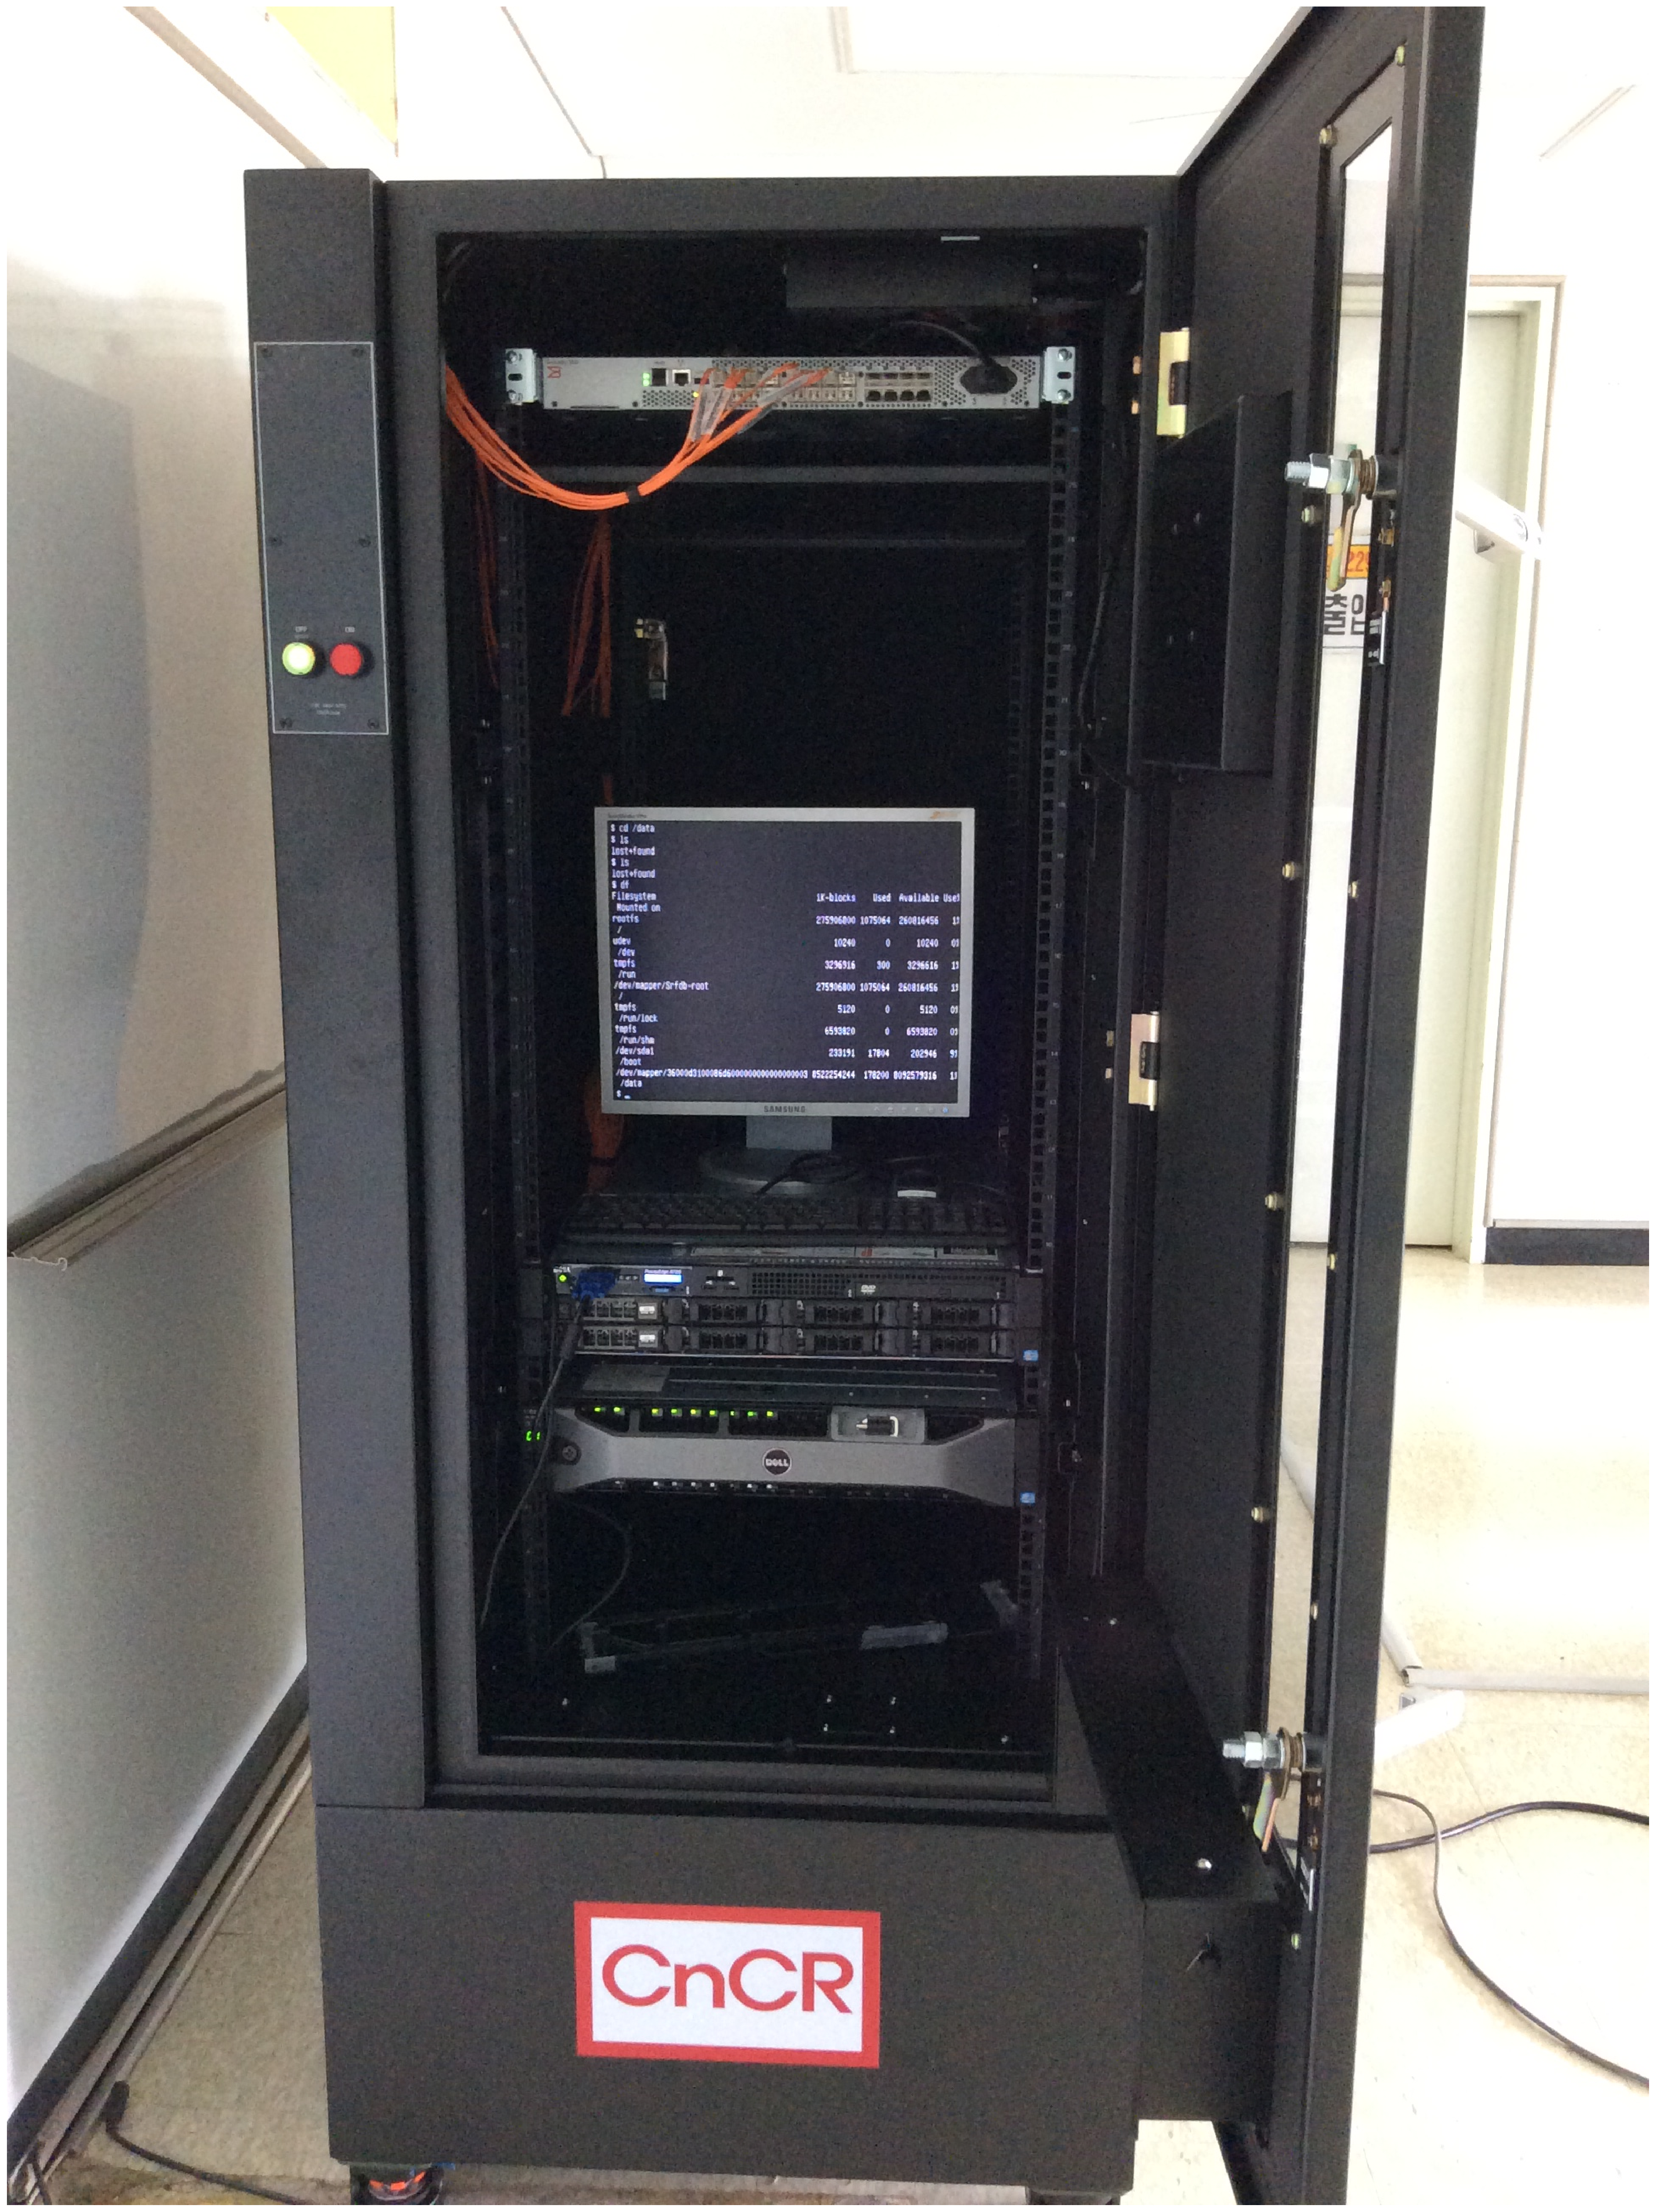
\includegraphics[width=0.85\textwidth]{./images/srfdb_fore.eps}
	\caption{SRF Storage 시스템 전면}
	\label{fig:srfdb_fore} 
\end{figure}

\begin{figure}[h!]
	\centering
	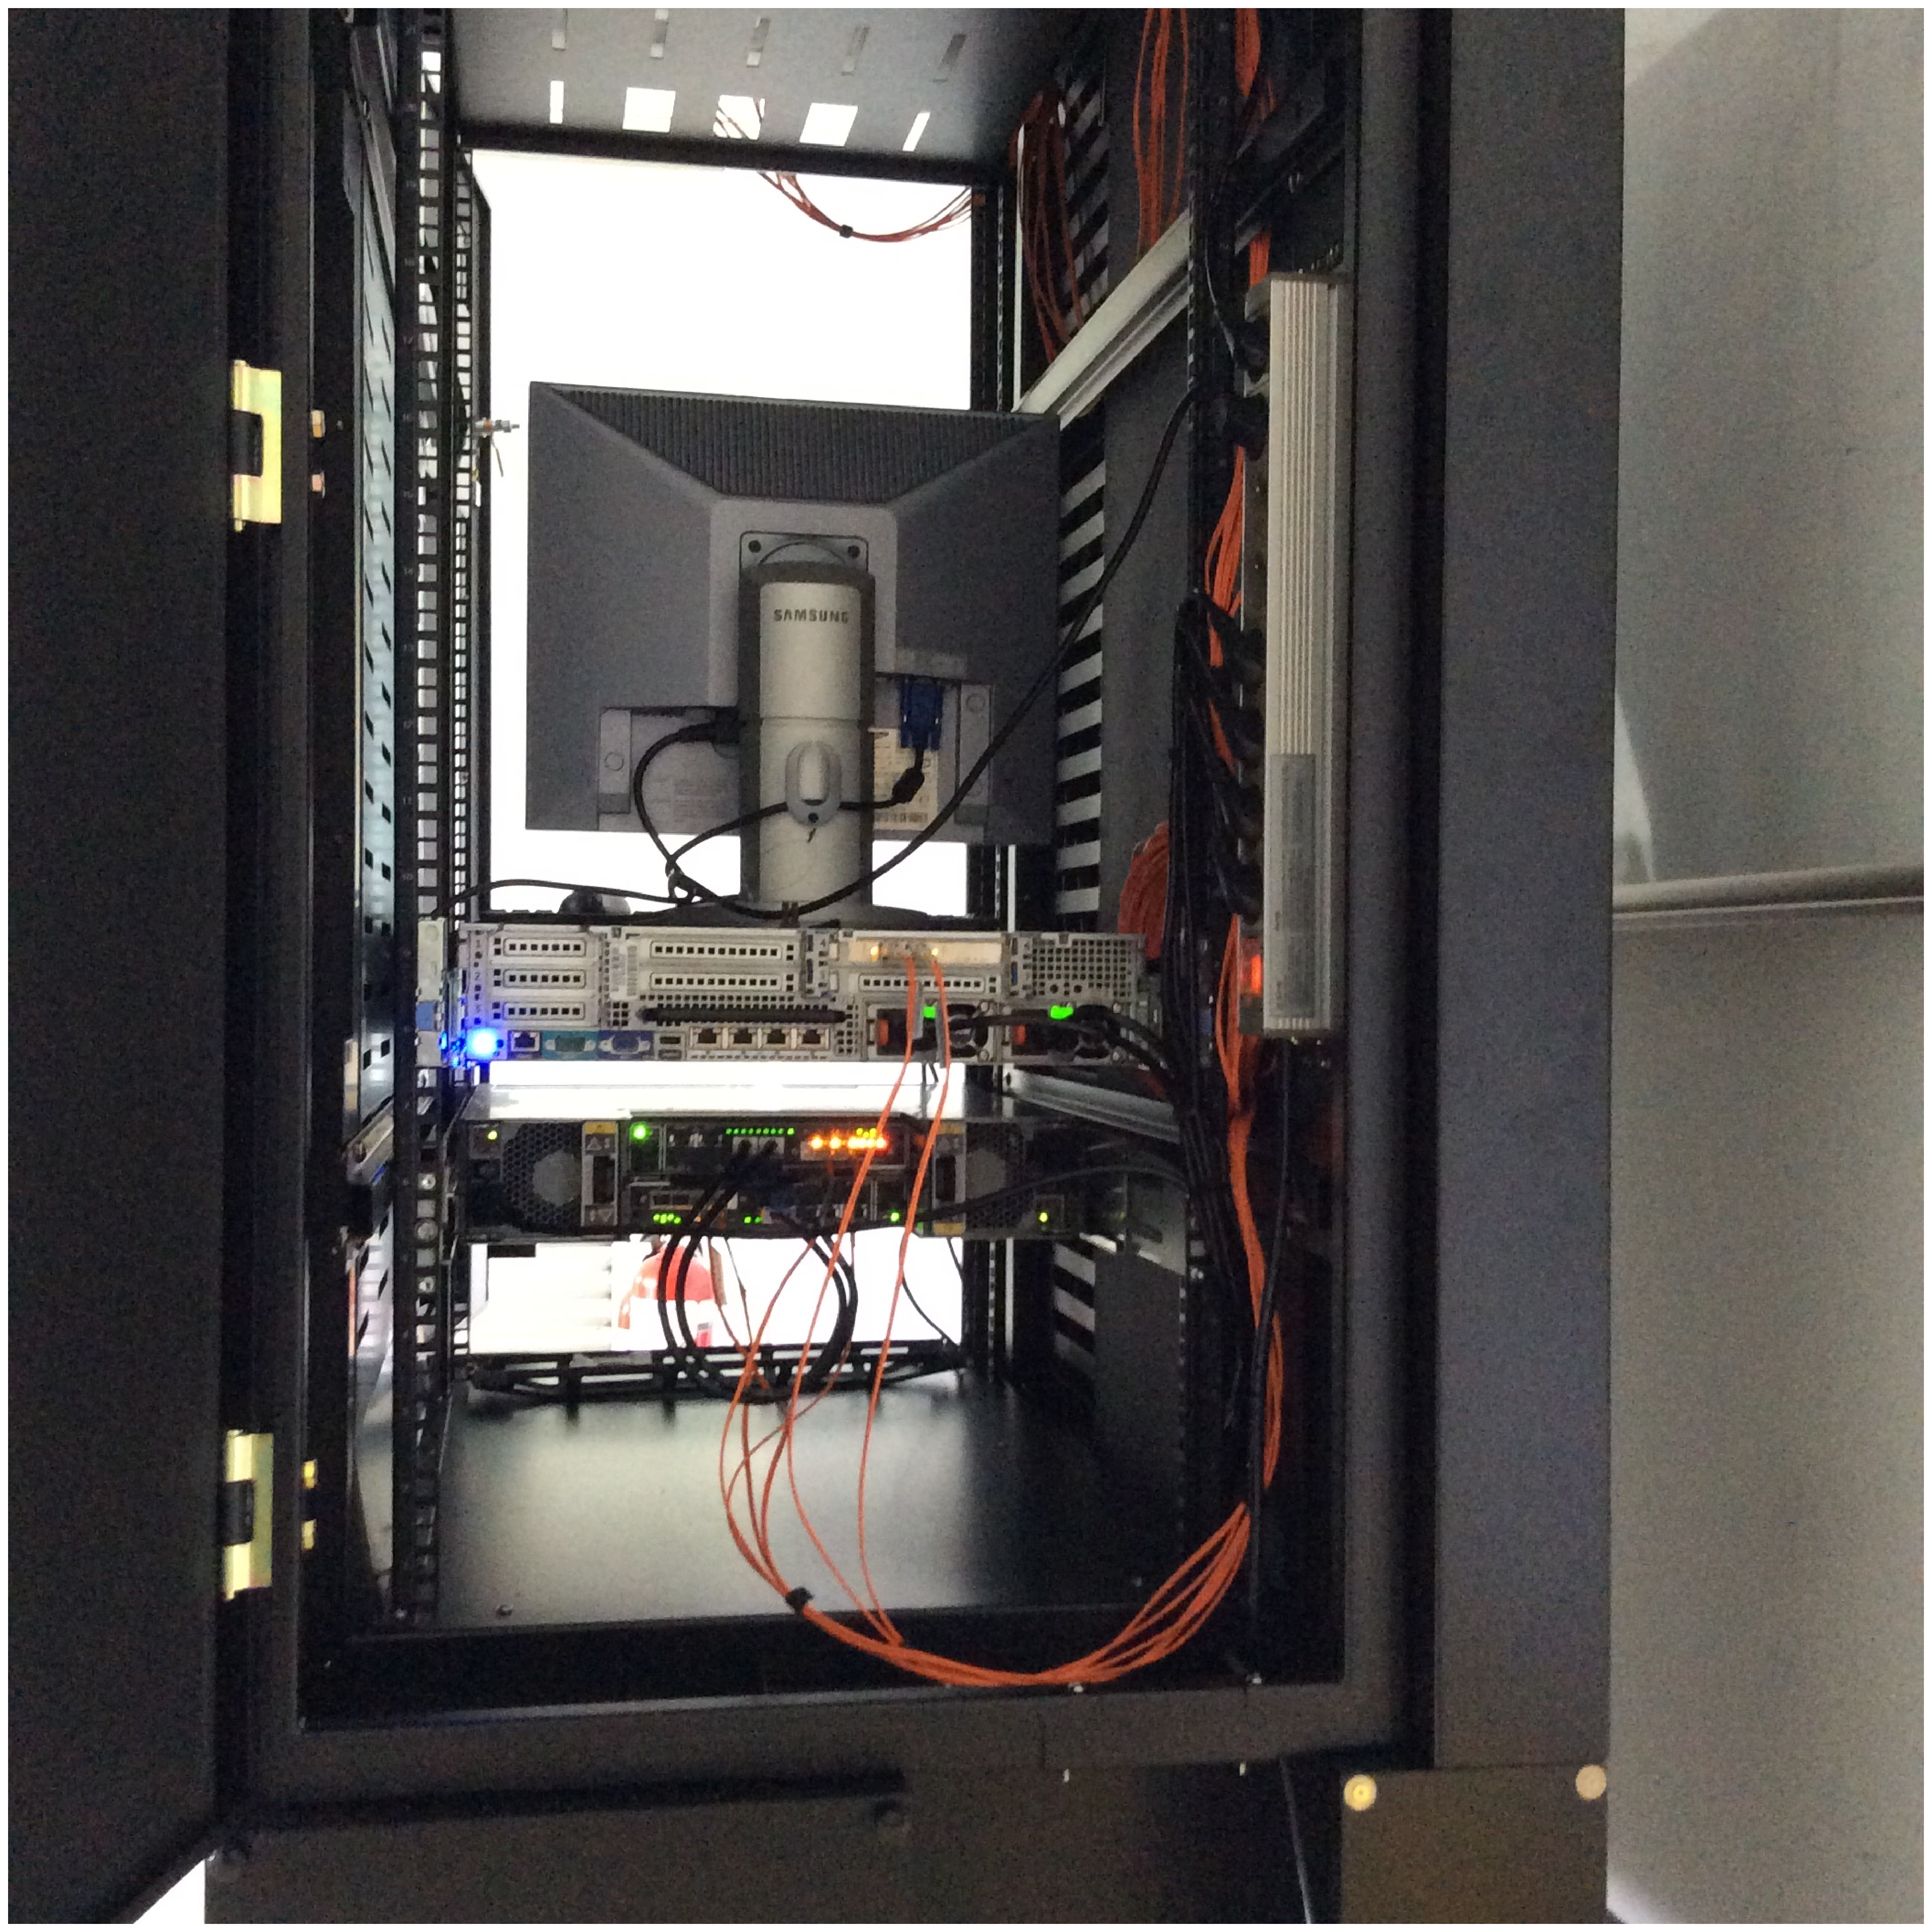
\includegraphics[width=0.85\textwidth]{./images/srfdb_back.eps}
	\caption{SRF Storage 시스템 후면}
	\label{fig:srfdb_back} 
\end{figure}

\clearpage

\bibliographystyle{unsrtnat}
\bibliography{./refs}

\end{document}

